\chapter{非定常 Navier--Stokes 方程组:层流}\label{chap:time-dependent-ns}

\begin{note}[非定常 Navier--Stokes 方程组]\label{note:time-dependent-ns-intro}
第\hyperref[chap:flow-equations]{2 章} 将非定常 Navier--Stokes 方程组\cref{eq:general-navier-stokes} 推导为描述不可压缩流体行为的模型.从数值模拟的角度看,需要区分层流和湍流.这两个概念并没有精确的定义.从模拟角度说,如果在合理的网格上能够表示或分辨流动中的所有结构,就认为该流动是层流.在这种情况下,可以采用 Galerkin 有限元法等标准空间离散方法进行模拟.

除空间离散外,非定常流动的模拟还需要对速度的时间导数进行离散.现有多种时间步进格式,它们会导出不同算法,用于数值求解非定常 Navier--Stokes 方程组.
\end{note}

\section{连续方程}\label{sec:time-dependent-ns-continuous}

\begin{note}[不可压缩 Navier--Stokes 方程组]\label{note:time-dependent-ns-equations}
本章讨论不可压缩 Navier--Stokes 方程组:
\begin{equation}\label{eq:time-dependent-ns-strong}
\begin{aligned}
  \partial_t\bm{u}-\nu\Delta\bm{u}
      +(\bm{u}\cdot\nabla)\bm{u}+\nabla p
    &=\bm{f},
      &&(t,\bm{x})\in(0,T]\times\Omega,\\
  \nabla\cdot\bm{u}&=0,
      &&(t,\bm{x})\in(0,T]\times\Omega,\\
  \bm{u}(0,\cdot)&=\bm{u}_0,
      &&\bm{x}\in\Omega,
\end{aligned}
\end{equation}
其中 $\Omega\subset\mathbb{R}^d$($d\in\{2,3\}$)为区域.以下只考虑有界 Lipschitz 区域,并假设 $\Omega$ 不随时间变化.为简化叙述,取齐次 Dirichlet 边界条件
\begin{equation}\label{eq:time-dependent-ns-dirichlet}
  \bm{u}=\bm{0}
  \qquad\text{于 }(0,T]\times\partial\Omega.
\end{equation}
\end{note}

\begin{note}[解的概念]\label{note:time-dependent-ns-solution-notions}
文献中有若干具有不同正则性等性质的(速度)解概念,例如经典解、强解、温和解、弱解和很弱解,参见\textcite{Farwig2014}.本章研究弱解.
\end{note}

\begin{note}[关于速度的弱方程]\label{note:time-dependent-ns-weak-velocity}
对于非定常不可压缩 Navier--Stokes 方程组,通常先将分析限制在适当的散度为零子空间内,并研究速度的存在性和唯一性;随后再研究相应压力的存在性.文献中关于速度的弱形式有多种写法.
\end{note}

\begin{note}[速度弱方程的第一种形式]\label{note:time-dependent-ns-weak-form-first}
与稳态方程一样,取 $V_{\mathrm{div}}$ 中的检验函数,将它们与\cref{eq:time-dependent-ns-strong} 的动量方程作内积,再对空间变量分部积分,可得到速度满足的常微分方程
\begin{equation}\label{eq:time-dependent-ns-weak-first}
\begin{aligned}
  \frac{\mathrm{d}}{\mathrm{d}t}(\bm{u},\bm{v})
    +\nu(\nabla\bm{u},\nabla\bm{v})
    +n(\bm{u},\bm{u},\bm{v})
    &=\langle\bm{f},\bm{v}\rangle_{V',V}
      &&\forall\bm{v}\in V_{\mathrm{div}},\\
  \bm{u}(0)&=\bm{u}_0.
\end{aligned}
\end{equation}
这里对时间的导数应按弱意义理解.这种弱方程形式可参见\textcite[第 158 页]{GiraultRaviart1979} 和\textcite[第 280 页]{Temam1984}.
\end{note}

\begin{definition}[Navier--Stokes 方程组的弱解或变分速度解]\label{def:time-dependent-ns-weak-velocity}
设 $\bm{f}\in L^2(0,T;V')$,$\bm{u}_0\in H_{\mathrm{div}}(\Omega)$,参见\textcite[第 158 页]{GiraultRaviart1979} 和\textcite[第 280 页]{Temam1984}.若
$\bm{u}\in L^2(0,T;V_{\mathrm{div}})$,且 $\bm{u}$ 在
$(C_0^1((0,T)))'$ 意义下满足\cref{eq:time-dependent-ns-weak-first},则称 $\bm{u}$ 为 Navier--Stokes 方程组的弱解或变分速度解.
\end{definition}



\begin{note}[速度弱方程的第二种形式]\label{note:time-dependent-ns-weak-form-second}
为得到这种形式,还需对时间积分并关于时间分部积分.也可以这样理解:将\cref{eq:time-dependent-ns-strong} 的动量方程乘以依赖时空变量的检验函数,在时空区域上积分,然后分部积分.

通常先使用光滑检验函数.要将结论推广到适当的 Lebesgue 空间和 Sobolev 空间中的检验函数,可利用光滑函数在这些空间中的稠密性,例如定理\hyperref[thm:appendix-a-38]{A.38}.具体地,取
$C^\infty_{0,\mathrm{div}}([0,T)\times\Omega)$ 中的检验函数.它们关于时间属于 $C_0^1([0,T))$,因此在终止时刻 $T$ 为零.按上述方法推导弱形式,可得
\begin{equation}\label{eq:time-dependent-ns-weak-integral}
\begin{gathered}
  \int_0^T\Bigl[
    -(\bm{u},\partial_t\symbf{\phi})
    +\nu(\nabla\bm{u},\nabla\symbf{\phi})
    +((\bm{u}\cdot\nabla)\bm{u},\symbf{\phi})
  \Bigr](\tau)\,\mathrm{d}\tau\\
  =\int_0^T
       \langle\bm{f},\symbf{\phi}\rangle_{V',V}(\tau)
       \,\mathrm{d}\tau
       +(\bm{u}_0,\symbf{\phi}(0,\cdot)),\\
  \forall\symbf{\phi}\in C^\infty_{0,\mathrm{div}}
       ([0,T)\times\Omega).
\end{gathered}
\end{equation}
注意,时间导数作用在检验函数上,而不是速度上.由于检验函数在终止时刻为零,时间分部积分在该时刻没有边界项.积分形\cref{eq:time-dependent-ns-weak-integral} 是常微分方程\cref{eq:time-dependent-ns-weak-first} 的积分表达.该形式的弱方程可参见\textcite{Galdi2000,Amann2000} 以及\textcite[第 263 页]{Sohr2001}.
\end{note}

\begin{definition}[Navier--Stokes 方程组的弱解或变分解]\label{def:time-dependent-ns-weak-solution}
设 $\bm{f}\in L^2(0,T;V')$,$\bm{u}_0\in H_{\mathrm{div}}(\Omega)$,参见\textcite{Galdi2000} 和\textcite[第 263 页]{Sohr2001}.若函数 $\bm{u}$ 满足以下条件,则称其为 Navier--Stokes 方程组的弱解或变分解:
\begin{itemize}
  \item $\bm{u}$ 满足\cref{eq:time-dependent-ns-weak-integral};
  \item $\bm{u}$ 具有如下正则性:
  \begin{equation}\label{eq:time-dependent-ns-weak-regularity}
    \bm{u}\in L^2(0,T;V_{\mathrm{div}})
      \cap L^\infty(0,T;H_{\mathrm{div}}(\Omega)).
  \end{equation}
\end{itemize}
\end{definition}

\begin{note}[证明弱解存在性的一般思路]\label{note:time-dependent-ns-existence-strategy}
证明弱解存在性的一般思路如下:
\begin{enumerate}
  \item 构造一列比\cref{eq:time-dependent-ns-weak-integral} 简单的问题,并证明当某个参数取适当极限时,这列问题收敛到\cref{eq:time-dependent-ns-weak-integral};
  \item 证明每个较简单的问题都有唯一解;
  \item 证明这列唯一解中的一个子列收敛到 Navier--Stokes 方程组的弱解.
\end{enumerate}
\end{note}

\begin{note}[较简单问题的构造方式]\label{note:time-dependent-ns-simpler-problems}
文献中已有多种构造较简单问题的方案,包括以下方法.
\begin{itemize}
  \item \textbf{Leray 正则化.}最早运用该方法得到的结果由 Leray 提出:
  \begin{itemize}
    \item 1933 年:$\Omega=\mathbb{R}^2$,\textcite{Leray1933};
    \item 1934 年:$\Omega$ 是 $\mathbb{R}^2$ 中固定的椭圆区域,\textcite{Leray1934a};
    \item 1934 年:$\Omega=\mathbb{R}^3$,\textcite{Leray1934b}.
  \end{itemize}
  最后一篇论文尤为重要.其中,简化方程采用对流项
  \[
    (\bm{u}_\varepsilon\cdot\nabla)\bm{u},
  \]
  取代 Navier--Stokes 方程组\cref{eq:time-dependent-ns-strong} 中的
  $(\bm{u}\cdot\nabla)\bm{u}$;这里 $\bm{u}_\varepsilon$ 是 $\bm{u}$ 在空间上以 $\varepsilon$ 为平均半径的平均:
  \[
    \begin{aligned}
    \bm{u}_\varepsilon(\bm{x})
      &=\frac{1}{\varepsilon^3}
        \int_\Omega
          \lambda\!\left(
            \frac{\lVert\bm{x}-\bm{y}\rVert_2^2}{\varepsilon^2}
          \right)
          \bm{u}(\bm{y})\,\mathrm{d}\bm{y},\\
    \lambda(s)&=\lambda_0 e^{1/(s-1)},\quad s\in(0,1).
    \end{aligned}
  \]
  其中 $\lambda_0$ 是使平均算子具有适当归一化的常数.采用对流场 $\bm{u}_\varepsilon$ 相当于对 Navier--Stokes 方程组作正则化;该方法研究极限 $\varepsilon\to0$.

  \item \textbf{空间半离散:Galerkin 方法.}\textcite{Hopf1951} 提出了上述一般思路中第一步所用的另一类较简单问题:在维数为 $n$ 的有限维空间中考虑\cref{eq:time-dependent-ns-weak-first} 或\cref{eq:time-dependent-ns-weak-integral},这就是 Galerkin 方法.方程形式仍与\cref{eq:time-dependent-ns-weak-first,eq:time-dependent-ns-weak-integral} 相同,但解和检验函数都取自同一个有限维空间.随后令 $n\to\infty$.由此得到的 Navier--Stokes 方程组弱解称为 Leray--Hopf 意义下的弱解.

  \item \textbf{时间半离散.}也可以通过时间离散构造较简单的问题,见\textcite[第 III.4 章]{Temam1984}.取极限时,再由离散时刻过渡到连续时间.

  \item \textbf{半群方法.}\textcite{Sohr1983} 提出了另一种证明弱解存在性的方法,亦可参见\textcite{Sohr2001}.该方法以半群为基础,见笔记\hyperref[note:semigroup-method]{8.16}.与 Leray 方法类似,它通过正则化对流项构造较简单的问题;正则化采用 Yosida 逼近,即湍流建模中微分滤波器的连续对应形式.

  \item \textbf{湍流模型.}湍流模型的复杂程度低于 Navier--Stokes 方程组,因而有助于流动模拟,也就提供了较简单的问题.湍流模型的极限也可能给出 Navier--Stokes 方程组的弱解;例如,对 Navier--Stokes-$\alpha$ 模型,可参见笔记\hyperref[note:navier-stokes-alpha-model]{8.203}.
\end{itemize}
下面将介绍一种基于 Galerkin 方法的处理途径.
\end{note}

\begin{note}[Galerkin 方法的起点:有限维子空间中的 Navier--Stokes 方程组]\label{note:time-dependent-galerkin-start}
Galerkin 方法的第一步,是在有限维空间中考虑 Navier--Stokes 方程组的弱形\cref{eq:time-dependent-ns-weak-first} 或\cref{eq:time-dependent-ns-weak-integral}.可以证明,存在空间 $C_{0,\mathrm{div}}^\infty(\Omega)$ 的一组基 $\{\bm{v}_l\}_{l=1}^\infty$,使这些基函数关于 $L^2(\Omega)$ 内积正交归一,见\textcite[引理 2.3]{Galdi2000}.据此定义有限维子空间
\[
  V_{\mathrm{div}}^n
    =\operatorname{span}\{\bm{v}_l^n\}_{l=1}^n
    \subset C_{0,\mathrm{div}}^\infty(\Omega).
\]
在该子空间中,将 Galerkin 方法用于\cref{eq:time-dependent-ns-weak-first},得到:求 $\bm{u}^n\in V_{\mathrm{div}}^n$,使得
\begin{equation}\label{eq:time-dependent-galerkin-problem}
\begin{aligned}
  (\partial_t\bm{u}^n,\bm{v}^n)
    +\nu(\nabla\bm{u}^n,\nabla\bm{v}^n)
    +n(\bm{u}^n,\bm{u}^n,\bm{v}^n)
    &=\langle\bm{f},\bm{v}^n\rangle_{V',V},\\
  \bm{u}^n(0)&=\bm{u}_0^n,\\
  &\hspace{3em}\forall\bm{v}^n\in V_{\mathrm{div}}^n.
\end{aligned}
\end{equation}
其中 $\bm{u}_0^n$ 是 $\bm{u}_0$ 在 $L^2(\Omega)$ 内积下投影到 $V_{\mathrm{div}}^n$ 上所得的正交投影.只要\cref{eq:time-dependent-galerkin-problem} 对这组基函数成立,它便对空间中的所有检验函数成立.将解表示为
\begin{equation}\label{eq:time-dependent-galerkin-expansion}
  \bm{u}^n(t,\bm{x})
    =\sum_{l=1}^n\alpha_l^n(t)\bm{v}_l^n(\bm{x}),
\end{equation}
代入\cref{eq:time-dependent-galerkin-problem},得到以下常微分方程组:
\begin{equation}\label{eq:time-dependent-galerkin-ode}
  \frac{\mathrm{d}\alpha_l^n}{\mathrm{d}t}
    +\sum_{j=1}^n a_{lj}\alpha_j^n
    +\sum_{j,k=1}^n n_{ljk}\alpha_j^n\alpha_k^n
    =f_l,\qquad l=1,\ldots,n,
\end{equation}
\begin{equation}\label{eq:time-dependent-galerkin-initial}
  \alpha_l^n(0)=u_{0l},\qquad l=1,\ldots,n,
\end{equation}
其中
\[
\begin{aligned}
  a_{lj}&=\nu(\nabla\bm{v}_j^n,\nabla\bm{v}_l^n),
  &n_{ljk}&=((\bm{v}_j^n\cdot\nabla)\bm{v}_k^n,\bm{v}_l^n)
            =n(\bm{v}_j^n,\bm{v}_k^n,\bm{v}_l^n),\\
  f_l&=\langle\bm{f},\bm{v}_l^n\rangle_{V',V},
  &u_{0l}&=(\bm{u}_0,\bm{v}_l^n).
\end{aligned}
\]
基函数正交归一并非必要,只是使表述更简洁.若基函数不正交归一,则\cref{eq:time-dependent-galerkin-ode} 的首项会出现 $V_{\mathrm{div}}^n$ 的 Gram 矩阵(质量矩阵).该矩阵可逆;左乘其逆矩阵后,首项与\cref{eq:time-dependent-galerkin-ode} 中的首项相同,而其他项会有所变化,参见\textcite[第 283 页]{Temam1984}.
\end{note}

\begin{lemma}[有限维问题的唯一可解性]\label{lem:time-dependent-galerkin-unique}
设 $\Omega\subset\mathbb{R}^d$($d\in\{2,3\}$)为有界 Lipschitz 区域,并假设 $\bm{f}$ 和 $\bm{u}_0$ 满足定义\hyperref[def:time-dependent-ns-weak-velocity]{7.6} 与定义\hyperref[def:time-dependent-ns-weak-solution]{7.8} 中的正则性条件.则系统\cref{eq:time-dependent-galerkin-expansion,eq:time-dependent-galerkin-ode,eq:time-dependent-galerkin-initial} 有唯一解,且该解在 $[0,T]$ 上绝对连续.下列先验估计成立:
\begin{equation}\label{eq:time-dependent-galerkin-estimate-sup}
  \sup_{t\in[0,T]}\lVert\bm{u}^n(t)\rVert_{L^2(\Omega)}^2
    \leq \lVert\bm{u}_0\rVert_{L^2(\Omega)}^2
      +\frac{1}{\nu}\lVert\bm{f}\rVert_{L^2(0,T;V')}^2,
\end{equation}
以及
\begin{equation}\label{eq:time-dependent-galerkin-estimate-energy}
\begin{aligned}
  \lVert\bm{u}^n(T)\rVert_{L^2(\Omega)}^2
    +\nu\lVert\nabla\bm{u}^n\rVert_{L^2(0,T;L^2(\Omega))}^2
    &\leq \lVert\bm{u}_0\rVert_{L^2(\Omega)}^2\\
    &\quad+\frac{1}{\nu}\lVert\bm{f}\rVert_{L^2(0,T;V')}^2.
\end{aligned}
\end{equation}
这两个估计关于 $n$ 一致.因此,$\bm{u}^n\in L^2(0,T;V_{\mathrm{div}})\cap L^\infty(0,T;H_{\mathrm{div}}(\Omega))$.
\begin{proof}
证明基于 Carathéodory 定理,见定理\hyperref[thm:appendix-a-50]{A.50}.因此,需要验证常微分方程组
\begin{equation}\label{eq:time-dependent-galerkin-coefficient-system}
  \frac{\mathrm{d}\symbf{\alpha}^n}{\mathrm{d}t}
    =\bm{F}(\symbf{\alpha}^n,t),\qquad t\in(0,T],
\end{equation}
右端满足 Lipschitz 条件,其中 $\bm{F}\in L^2(0,T)$.若 $\bm{F}$ 在 $[0,T]$ 上连续,就可以应用著名的 Peano 定理;但由于此处的正则性条件,需要使用 Carathéodory 定理.

右端中,系数 $\alpha_l^n$ 以一次和二次形式出现.因此,右端关于这些系数满足 Lipschitz 条件.由 Carathéodory 定理可知,存在一个最大区间 $[0,t_n]$($0<t_n\leq T$),使得解 $\bm{u}^n(t,\bm{x})$ 在该区间上局部存在且唯一,并且绝对连续.若 $t_n<T$,则 $\bm{u}^n(t)$ 在 $t\to t_n$ 时会发散.

下面证明先验估计\cref{eq:time-dependent-galerkin-estimate-sup,eq:time-dependent-galerkin-estimate-energy},由此排除上述情形,得到 $t_n=T$.

对任意 $t\in(0,T)$,在\cref{eq:time-dependent-galerkin-problem} 中取检验函数 $\bm{v}^n=\bm{u}^n(t,\bm{x})$.利用第一项的乘积求导法则
\begin{equation}\label{eq:time-dependent-galerkin-product-rule}
\begin{aligned}
  \frac{\mathrm{d}}{\mathrm{d}t}
    \lVert\bm{u}^n(t)\rVert_{L^2(\Omega)}^2
  &=\frac{\mathrm{d}}{\mathrm{d}t}
      (\bm{u}^n(t),\bm{u}^n(t))\\
  &=(\partial_t\bm{u}^n(t),\bm{u}^n(t))
      +(\bm{u}^n(t),\partial_t\bm{u}^n(t))\\
  &=2(\partial_t\bm{u}^n(t),\bm{u}^n(t)),
\end{aligned}
\end{equation}
再利用 Navier--Stokes 对流项的消失性质\cref{eq:steady-ns-convection-zero-conv}、对偶配对估计和 Young 不等式\hyperref[eq:appendix-a-5]{(A.5)},可得
\begin{equation}\label{eq:time-dependent-galerkin-energy-step}
\begin{aligned}
  \frac{1}{2}\frac{\mathrm{d}}{\mathrm{d}t}
      \lVert\bm{u}^n(t)\rVert_{L^2(\Omega)}^2
    +\nu\lVert\nabla\bm{u}^n(t)\rVert_{L^2(\Omega)}^2
  &=\langle\bm{f}(t),\bm{u}^n(t)\rangle_{V',V}\\
  &\leq \lVert\bm{f}(t)\rVert_{V'}
      \lVert\nabla\bm{u}^n(t)\rVert_{L^2(\Omega)}\\
  &\leq \frac{1}{2\nu}\lVert\bm{f}(t)\rVert_{V'}^2\\
  &\quad +\frac{\nu}{2}\lVert\nabla\bm{u}^n(t)\rVert_{L^2(\Omega)}^2.
\end{aligned}
\end{equation}
于是
\begin{equation}\label{eq:time-dependent-galerkin-energy-inequality}
  \frac{\mathrm{d}}{\mathrm{d}t}
      \lVert\bm{u}^n(t)\rVert_{L^2(\Omega)}^2
    +\nu\lVert\nabla\bm{u}^n(t)\rVert_{L^2(\Omega)}^2
    \leq\frac{1}{\nu}\lVert\bm{f}(t)\rVert_{V'}^2.
\end{equation}
在任意区间 $[0,t]$($t\leq T$)上积分,并使用 $L^2(\Omega)$ 正交投影的估计\hyperref[eq:appendix-c-26]{(C.26)},得到
\[
  \begin{aligned}
  \lVert\bm{u}^n(t)\rVert_{L^2(\Omega)}^2
    &\leq \lVert\bm{u}_0^n\rVert_{L^2(\Omega)}^2\\
    &\quad+\frac{1}{\nu}
       \int_0^t\lVert\bm{f}(\tau)\rVert_{V'}^2\,\mathrm{d}\tau\\
    &\leq \lVert\bm{u}_0\rVert_{L^2(\Omega)}^2\\
    &\quad+\frac{1}{\nu}\lVert\bm{f}\rVert_{L^2(0,t;V')}^2.
  \end{aligned}
\]
在 $[0,T]$ 上取上确界,即得先验估计\cref{eq:time-dependent-galerkin-estimate-sup}.又因为 $\bm{u}^n\in H_{\mathrm{div}}(\Omega)$,所以 $\bm{u}^n\in L^\infty(0,T;H_{\mathrm{div}}(\Omega))$.

再将\cref{eq:time-dependent-galerkin-energy-inequality} 在 $[0,T]$ 上积分,同理可得\cref{eq:time-dependent-galerkin-estimate-energy}.由于 $\bm{u}^n\in V_{\mathrm{div}}$,特别有 $\bm{u}^n\in L^2(0,T;V_{\mathrm{div}})$.
\end{proof}


\end{lemma}



\begin{corollary}[弱收敛]\label{cor:time-dependent-galerkin-weak-convergence}
存在子列 $\{\bm{u}^{n_\ell}\}_{\ell=1}^\infty$ 及函数
$\bm{u}\in L^2(0,T;V_{\mathrm{div}})\cap L^\infty(0,T;H_{\mathrm{div}}(\Omega))$,使得
\[
  \bm{u}^{n_\ell}\stackrel{*}{\rightharpoonup}\bm{u}
    \quad\text{于 }L^\infty(0,T;H_{\mathrm{div}}(\Omega)),\\
  \bm{u}^{n_\ell}\rightharpoonup\bm{u}
    \quad\text{于 }L^2(0,T;V_{\mathrm{div}})
\]
($\ell\to\infty$).
\begin{proof}
由\lemref{lem:time-dependent-galerkin-unique} 可知,序列
$\{\bm{u}^n\}_{n=1}^\infty$ 在 $L^2(0,T;V_{\mathrm{div}})$ 中一致有界.该空间是 Hilbert 空间,因而是自反 Banach 空间;于是存在一个子列弱收敛到某个
$\bm{u}_1\in L^2(0,T;V_{\mathrm{div}})$,见注记\hyperref[note:appendix-a-58]{A.58}.此弱极限唯一.

空间 $L^1(0,T;H_{\mathrm{div}}(\Omega))$ 是可分 Banach 空间,其对偶空间为 $L^\infty(0,T;H_{\mathrm{div}}(\Omega))$.由\lemref{lem:time-dependent-galerkin-unique} 可知,$\{\bm{u}^n\}_{n=1}^\infty$ 在该对偶空间中一致有界.因此存在一个子列弱星收敛到某个
$\bm{u}_2\in L^\infty(0,T;H_{\mathrm{div}}(\Omega))$,见注记\hyperref[note:appendix-a-58]{A.58}.此极限同样唯一.

由于
\[
  \{\bm{u}^n\}_{n=1}^\infty
    \subset L^2(0,T;V_{\mathrm{div}})
      \cap L^\infty(0,T;H_{\mathrm{div}}(\Omega)),
\]
且这两个空间都是完备的,因此
  \[
  \begin{aligned}
  \bm{u}_1,\bm{u}_2
    &\in L^2(0,T;V_{\mathrm{div}})\\
    &\quad\cap L^\infty(0,T;H_{\mathrm{div}}(\Omega)).
  \end{aligned}
\]
由极限的唯一性可知,$\bm{u}_1=\bm{u}_2=\bm{u}$.
\end{proof}
\end{corollary}

\begin{note}[弱收敛的后果:线性项的收敛]\label{note:time-dependent-galerkin-linear-convergence}
为简化记号,以下仍用 $\{\bm{u}^n\}_{n=1}^\infty$ 表示\corref{cor:time-dependent-galerkin-weak-convergence} 中的子列.考虑 Galerkin 问题\cref{eq:time-dependent-galerkin-problem} 的解,任取 $\bm{v}\in V_{\mathrm{div}}$,并取 $\varphi\in C_0^\infty((0,T))$.分部积分得
\[
  \int_0^T(\partial_t\bm{u}^n(t),\bm{v})\varphi(t)\,\mathrm{d}t
    =-\int_0^T(\bm{u}^n(t),\bm{v})
        \frac{\mathrm{d}}{\mathrm{d}t}\varphi(t)\,\mathrm{d}t.
\]
由于 $\bm{u}^n\stackrel{*}{\rightharpoonup}\bm{u}$ 于
$L^\infty(0,T;H_{\mathrm{div}}(\Omega))$,且
$\frac{\mathrm{d}}{\mathrm{d}t}\varphi\in L^1(0,T)$,有
\[
\begin{aligned}
  \lim_{n\to\infty}-\int_0^T(\bm{u}^n(t),\bm{v})
      \frac{\mathrm{d}}{\mathrm{d}t}\varphi(t)\,\mathrm{d}t
    &=\int_0^T(\bm{u}(t),\bm{v})
      \frac{\mathrm{d}}{\mathrm{d}t}\varphi(t)\,\mathrm{d}t\\
    &=\int_0^T(\partial_t\bm{u}(t),\bm{v})
      \varphi(t)\,\mathrm{d}t.
\end{aligned}
\]
因此,对所有 $\bm{v}\in V_{\mathrm{div}}$,$\bm{u}$ 满足\cref{eq:time-dependent-ns-weak-first} 中时间导数项的弱形式.

对黏性项,由 $\bm{u}^n\rightharpoonup\bm{u}$ 于 $L^2(0,T;V_{\mathrm{div}})$,并取 $\varphi\in L^2(0,T)$,可知对所有 $\bm{v}\in V_{\mathrm{div}}$ 和 $\varphi\in C_0^\infty((0,T))$,
\begin{equation}\label{eq:time-dependent-galerkin-viscous-convergence}
  \lim_{n\to\infty}\int_0^T
     (\nu\nabla\bm{u}^n,\nabla\bm{v})\varphi(t)\,\mathrm{d}t
    =\int_0^T(\nu\nabla\bm{u},\nabla\bm{v})
       \varphi(t)\,\mathrm{d}t.
\end{equation}
这就是\cref{eq:time-dependent-ns-weak-first} 中黏性项的弱形式.

要证明 $\bm{u}$ 是 Navier--Stokes 方程组的弱解,还需证明非线性对流项收敛:
\[
  n(\bm{u}^n,\bm{u}^n,\bm{v})
    \longrightarrow n(\bm{u},\bm{u},\bm{v}).
\]
证明该性质有多种方法,例如\textcite[第 285 页]{Temam1984} 所用的 Fourier 变换,或\textcite{Galdi2000} 所用的特殊 Friedrichs 不等式.下面概述\textcite[第 161 页]{GiraultRaviart1979} 的证明方法.
\end{note}

\begin{lemma}[非线性对流项差的估计]\label{lem:time-dependent-convection-difference}
设 $\bm{u},\bar{\bm{u}}\in L^2(0,T;V_{\mathrm{div}})\cap L^\infty(0,T;H_{\mathrm{div}}(\Omega))$,$\bm{v}\in V_{\mathrm{div}}$,且 $r\in[1,4/3)$.则
\begin{equation}\label{eq:time-dependent-convection-difference-estimate}
\begin{aligned}
  &\int_0^T
    \bigl|n(\bm{u},\bm{u},\bm{v})
       -n(\bar{\bm{u}},\bar{\bm{u}},\bm{v})\bigr|^r\,\mathrm{d}t\\
  &\quad\leq C\lVert\nabla\bm{v}\rVert_{L^2(\Omega)}^r
    \Bigl(\lVert\bm{u}\rVert_{L^\infty(0,T;L^2(\Omega))}^{r/4}
       +\lVert\bar{\bm{u}}\rVert_{L^\infty(0,T;L^2(\Omega))}^{r/4}\Bigr)\\
  &\qquad\times
    \lVert\bm{u}-\bar{\bm{u}}\rVert
       _{L^{r/(4-3r)}(0,T;L^2(\Omega))}^{r/4}\\
  &\qquad\times\Bigl(
       \lVert\nabla\bm{u}\rVert_{L^2(0,T;L^2(\Omega))}^{3r/2}
       +\lVert\nabla\bar{\bm{u}}\rVert_{L^2(0,T;L^2(\Omega))}^{3r/2}
       \Bigr).
\end{aligned}
\end{equation}
\begin{proof}
在差中加减同一项,应用三角不等式和非线性对流项的斜对称性\cref{eq:steady-ns-conv-skew},得到
\[
\begin{aligned}
  &\bigl|n(\bm{u},\bm{u},\bm{v})
      -n(\bar{\bm{u}},\bar{\bm{u}},\bm{v})\bigr|\\
  &=\bigl|n(\bm{u}-\bar{\bm{u}},\bm{u},\bm{v})
      -n(\bar{\bm{u}},\bar{\bm{u}}-\bm{u},\bm{v})\bigr|\\
  &\leq\bigl|n(\bm{u}-\bar{\bm{u}},\bm{u},\bm{v})\bigr|
      +\bigl|n(\bar{\bm{u}},\bar{\bm{u}}-\bm{u},\bm{v})\bigr|\\
  &=\bigl|n(\bm{u}-\bar{\bm{u}},\bm{v},\bm{u})\bigr|
      +\bigl|n(\bar{\bm{u}},\bm{v},\bar{\bm{u}}-\bm{u})\bigr|.
\end{aligned}
\]
证明的目标是导出关于 $\bm{u}-\bar{\bm{u}}$ 的尽可能弱的范数估计.

接下来,应用广义 Hölder 不等\cref{eq:steady-ns-generalized-holder}(取 $p=r=1/4$、$q=2$)、Sobolev 嵌入定理\hyperref[eq:appendix-a-15]{(A.15)}(取 $m=3/4$、$p=2$、$q=4$),以及 Sobolev 空间的插值估计\hyperref[eq:appendix-a-13]{(A.13)},得到
\[
\begin{aligned}
  &\bigl|n(\bm{u},\bm{u},\bm{v})
      -n(\bar{\bm{u}},\bar{\bm{u}},\bm{v})\bigr|\\
  &\leq \lVert\bm{u}-\bar{\bm{u}}\rVert_{L^4(\Omega)}
       \lVert\nabla\bm{v}\rVert_{L^2(\Omega)}
       \lVert\bm{u}\rVert_{L^4(\Omega)}\\
  &\qquad+\lVert\bar{\bm{u}}\rVert_{L^4(\Omega)}
       \lVert\nabla\bm{v}\rVert_{L^2(\Omega)}
       \lVert\bm{u}-\bar{\bm{u}}\rVert_{L^4(\Omega)}\\
  &=\lVert\nabla\bm{v}\rVert_{L^2(\Omega)}
      \lVert\bm{u}-\bar{\bm{u}}\rVert_{L^4(\Omega)}
      \Bigl(\lVert\bm{u}\rVert_{L^4(\Omega)}
        +\lVert\bar{\bm{u}}\rVert_{L^4(\Omega)}\Bigr)\\
  &\leq C\lVert\nabla\bm{v}\rVert_{L^2(\Omega)}
      \lVert\bm{u}-\bar{\bm{u}}\rVert_{H^{3/4}(\Omega)}
      \Bigl(\lVert\bm{u}\rVert_{H^{3/4}(\Omega)}
        +\lVert\bar{\bm{u}}\rVert_{H^{3/4}(\Omega)}\Bigr)\\
  &\leq C\lVert\nabla\bm{v}\rVert_{L^2(\Omega)}
      \lVert\bm{u}-\bar{\bm{u}}\rVert_{L^2(\Omega)}^{1/4}
      \lVert\nabla(\bm{u}-\bar{\bm{u}})\rVert_{L^2(\Omega)}^{3/4}\\
  &\qquad\times\Bigl(
       \lVert\bm{u}\rVert_{L^2(\Omega)}^{1/4}
       \lVert\nabla\bm{u}\rVert_{L^2(\Omega)}^{3/4}
       +\lVert\bar{\bm{u}}\rVert_{L^2(\Omega)}^{1/4}
       \lVert\nabla\bar{\bm{u}}\rVert_{L^2(\Omega)}^{3/4}
       \Bigr).
\end{aligned}
\]
应用广义 Hölder 不等式时,对 $\bm{v}$ 使用了其最大正则性;另外两项以相同方式处理.还要注意,若应用 Poincaré 不等式,关于差 $\bm{u}-\bar{\bm{u}}$ 的范数会变强.

取 $r\in[1,4/3)$,于是
\begin{equation}\label{eq:time-dependent-convection-difference-time-integral}
\begin{aligned}
  &\int_0^T
    \bigl|n(\bm{u},\bm{u},\bm{v})
       -n(\bar{\bm{u}},\bar{\bm{u}},\bm{v})\bigr|^r\,\mathrm{d}t\\
  &\leq C\lVert\nabla\bm{v}\rVert_{L^2(\Omega)}^r
       \int_0^T\Bigl[
       \lVert\bm{u}-\bar{\bm{u}}\rVert_{L^2(\Omega)}^{r/4}
       \lVert\nabla(\bm{u}-\bar{\bm{u}})\rVert_{L^2(\Omega)}^{3r/4}\\
  &\qquad\qquad\times\Bigl(
       \lVert\bm{u}\rVert_{L^2(\Omega)}^{1/4}
       \lVert\nabla\bm{u}\rVert_{L^2(\Omega)}^{3/4}
       +\lVert\bar{\bm{u}}\rVert_{L^2(\Omega)}^{1/4}
       \lVert\nabla\bar{\bm{u}}\rVert_{L^2(\Omega)}^{3/4}
       \Bigr)\Bigr]^r\,\mathrm{d}t.
\end{aligned}
\end{equation}
对其中两个项关于时间取上确界,并利用
\[
  ab+cd\leq(a+c)(b+d),\qquad a,b,c,d\geq0,
\]
以及当 $a,b\geq0$ 且 $q\geq1$ 时 $(a+b)^q\leq C(a^q+b^q)$,可将积分估计为
\begin{equation}\label{eq:time-dependent-convection-difference-sup}
\begin{aligned}
  &\int_0^T\Bigl[
       \lVert\bm{u}-\bar{\bm{u}}\rVert_{L^2(\Omega)}^{r/4}
       \lVert\nabla(\bm{u}-\bar{\bm{u}})\rVert_{L^2(\Omega)}^{3r/4}\\
  &\qquad\times\Bigl(
       \lVert\bm{u}\rVert_{L^2(\Omega)}^{1/4}
       \lVert\nabla\bm{u}\rVert_{L^2(\Omega)}^{3/4}
       +\lVert\bar{\bm{u}}\rVert_{L^2(\Omega)}^{1/4}
       \lVert\nabla\bar{\bm{u}}\rVert_{L^2(\Omega)}^{3/4}
       \Bigr)\Bigr]^r\,\mathrm{d}t\\
  &\leq C\Bigl(
       \lVert\bm{u}\rVert_{L^\infty(0,T;L^2(\Omega))}^{r/4}
       +\lVert\bar{\bm{u}}\rVert_{L^\infty(0,T;L^2(\Omega))}^{r/4}
       \Bigr)\\
  &\quad\times\int_0^T
       \lVert\bm{u}-\bar{\bm{u}}\rVert_{L^2(\Omega)}^{r/4}
       \lVert\nabla(\bm{u}-\bar{\bm{u}})\rVert_{L^2(\Omega)}^{3r/4}\\
  &\qquad\times\Bigl(
       \lVert\nabla\bm{u}\rVert_{L^2(\Omega)}^{3r/4}
       +\lVert\nabla\bar{\bm{u}}\rVert_{L^2(\Omega)}^{3r/4}
       \Bigr)\,\mathrm{d}t.
\end{aligned}
\end{equation}
再看积分本身.利用三角不等式(在 Lebesgue 空间中也称 Minkowski 不等式),并应用 $q\in(0,1)$ 时的不等式
\[
  (a+b)^q\leq a^q+b^q,\qquad a,b\geq0,
\]
(它可由\hyperref[eq:appendix-a-4]{(A.4)} 的左侧不等式推出),再结合 Young 不等式\hyperref[eq:appendix-a-5]{(A.5)},得到
\begin{equation}\label{eq:time-dependent-convection-difference-gradient}
\begin{aligned}
  &\int_0^T
       \lVert\bm{u}-\bar{\bm{u}}\rVert_{L^2(\Omega)}^{r/4}
       \lVert\nabla(\bm{u}-\bar{\bm{u}})\rVert_{L^2(\Omega)}^{3r/4}\\
  &\qquad\times\Bigl(
       \lVert\nabla\bm{u}\rVert_{L^2(\Omega)}^{3r/4}
       +\lVert\nabla\bar{\bm{u}}\rVert_{L^2(\Omega)}^{3r/4}
       \Bigr)\,\mathrm{d}t\\
  &\leq C\int_0^T
       \lVert\bm{u}-\bar{\bm{u}}\rVert_{L^2(\Omega)}^{r/4}
       \Bigl(
       \lVert\nabla\bm{u}\rVert_{L^2(\Omega)}^{3r/4}
       +\lVert\nabla\bar{\bm{u}}\rVert_{L^2(\Omega)}^{3r/4}
       \Bigr)^2\,\mathrm{d}t\\
  &\leq C\int_0^T
       \lVert\bm{u}-\bar{\bm{u}}\rVert_{L^2(\Omega)}^{r/4}
       \Bigl(
       \lVert\nabla\bm{u}\rVert_{L^2(\Omega)}^{3r/2}
       +\lVert\nabla\bar{\bm{u}}\rVert_{L^2(\Omega)}^{3r/2}
       \Bigr)\,\mathrm{d}t.
\end{aligned}
\end{equation}
当 $r\leq4/3$ 时该积分有定义:依假设,第一项属于 $L^\infty(0,T)$,梯度范数属于 $L^2(0,T)$.

最后应用 Hölder 不等式\hyperref[eq:appendix-a-9]{(A.9)}.由于 $\bm{u},\bar{\bm{u}}\in L^2(0,T;V_{\mathrm{div}})$,括号中各项的幂次应为 $2$.因此,在\hyperref[eq:appendix-a-9]{(A.9)} 中取 $p=4/(3r)>1$、$q=4/(4-3r)$,可得
\[
\begin{aligned}
  &\int_0^T
       \lVert\bm{u}-\bar{\bm{u}}\rVert_{L^2(\Omega)}^{r/4}
       \Bigl(
       \lVert\nabla\bm{u}\rVert_{L^2(\Omega)}^{3r/2}
       +\lVert\nabla\bar{\bm{u}}\rVert_{L^2(\Omega)}^{3r/2}
       \Bigr)\,\mathrm{d}t\\
  &\leq
       \Biggl(\int_0^T
       \lVert\bm{u}-\bar{\bm{u}}\rVert_{L^2(\Omega)}^{r/(4-3r)}
       \,\mathrm{d}t\Biggr)^{(4-3r)/4}\\
  &\quad\times\Biggl[
       \Biggl(\int_0^T\lVert\nabla\bm{u}\rVert_{L^2(\Omega)}^2
          \,\mathrm{d}t\Biggr)^{3r/4}
       +\Biggl(\int_0^T\lVert\nabla\bar{\bm{u}}\rVert_{L^2(\Omega)}^2
          \,\mathrm{d}t\Biggr)^{3r/4}
       \Biggr].
\end{aligned}
\]
将此估计代入\cref{eq:time-dependent-convection-difference-time-integral,eq:time-dependent-convection-difference-sup,eq:time-dependent-convection-difference-gradient},即得\cref{eq:time-dependent-convection-difference-estimate}.
\end{proof}
\end{lemma}

\begin{lemma}[非线性对流项的收敛]\label{lem:time-dependent-convection-convergence}
对任意 $\bm{v}\in V_{\mathrm{div}}$ 和 $\varphi\in C_0^\infty((0,T))$,有
\begin{equation}\label{eq:time-dependent-nonlinear-convection-limit}
  \begin{gathered}
  \lim_{n\to\infty}\int_0^T
       n(\bm{u}^n(t),\bm{u}^n(t),\bm{v})\varphi(t)\,\mathrm{d}t
       \\
  =\int_0^T n(\bm{u}(t),\bm{u}(t),\bm{v})
       \varphi(t)\,\mathrm{d}t,
  \end{gathered}
\end{equation}
其中 $\bm{u}^n\rightharpoonup\bm{u}$ 于 $L^2(0,T;V_{\mathrm{div}})$.
\begin{proof}
这里只给出证明梗概.首先证明,对某个 $\sigma\in(0,1/4)$,有
\[
  \bm{u}^n\in H^\sigma(0,T;H_{\mathrm{div}}(\Omega)),
\]
其中 $H^\sigma(0,T;H_{\mathrm{div}}(\Omega))$ 的 Gagliardo 范数为
\[
\begin{aligned}
  \lVert\bm{u}^n\rVert_{H^\sigma(0,T;H_{\mathrm{div}}(\Omega))}^2
  ={}&\lVert\bm{u}^n\rVert_{L^2(0,T;H_{\mathrm{div}}(\Omega))}^2\\
   &+\int_0^T\int_0^T
      \frac{\lVert\bm{u}^n(t)-\bm{u}^n(s)\rVert_{L^2(\Omega)}^2}
           {|t-s|^{1+2\sigma}}\,\mathrm{d}s\,\mathrm{d}t.
\end{aligned}
\]
证明这一正则性性质的过程较长,可参见\textcite[第 V 章,引理 1.7]{GiraultRaviart1979}.

接下来,应用 Lions--Aubin 紧性定理可知
\[
  L^2(0,T;V_{\mathrm{div}})\cap
  H^\sigma(0,T;H_{\mathrm{div}}(\Omega))
  \hookrightarrow\hookrightarrow L^2(0,T;H_{\mathrm{div}}(\Omega)),
\]
亦可参见\textcite[第 V 章,引理 1.3]{GiraultRaviart1979} 对这一性质的直接证明.由\lemref{lem:time-dependent-galerkin-unique} 和上述正则性可知,$\{\bm{u}^n\}_{n=1}^\infty$ 在
$L^2(0,T;V_{\mathrm{div}})\cap H^\sigma(0,T;H_{\mathrm{div}}(\Omega))$ 中有界.因此,由紧嵌入可知,存在一个子列,它在 $L^2(0,T;H_{\mathrm{div}}(\Omega))$ 中为 Cauchy 列.由于该空间完备,此子列强收敛到某个
$\bm{u}\in L^2(0,T;H_{\mathrm{div}}(\Omega))$.极限的唯一性以及该极限属于 $L^2(0,T;V_{\mathrm{div}})$,说明它与\corref{cor:time-dependent-galerkin-weak-convergence} 中的极限相同.

在\cref{eq:time-dependent-convection-difference-estimate} 中取 $\bar{\bm{u}}=\bm{u}^n$、$r=8/7$,则
\[
  \begin{aligned}
  \lVert\bm{u}-\bm{u}^n\rVert_{L^{r/(4-3r)}(0,T;L^2(\Omega))}^{r/4}
    &=\lVert\bm{u}-\bm{u}^n\rVert_{L^2(0,T;L^2(\Omega))}^{2/7}\\
    &\longrightarrow0\qquad(n\to\infty).
  \end{aligned}
\]
因此,由\cref{eq:time-dependent-convection-difference-estimate} 可得
\[
  \lim_{n\to\infty}\int_0^T
    \bigl|n(\bm{u},\bm{u},\bm{v})
        -n(\bm{u}^n,\bm{u}^n,\bm{v})\bigr|^{8/7}
       \,\mathrm{d}t=0.
\]
既然该差在 $L^{8/7}(0,T)$ 中收敛,它也在 $L^1(0,T)$ 中收敛.因此
\[
\begin{aligned}
  &\left|\int_0^T
      \bigl(n(\bm{u}^n,\bm{u}^n,\bm{v})
         -n(\bm{u},\bm{u},\bm{v})\bigr)\varphi(t)\,\mathrm{d}t\right|\\
  &\qquad\leq\lVert\varphi\rVert_{L^\infty(0,T)}
       \int_0^T
        \bigl|n(\bm{u}^n,\bm{u}^n,\bm{v})
          -n(\bm{u},\bm{u},\bm{v})\bigr|\,\mathrm{d}t
       \longrightarrow0,
\end{aligned}
\]
这就证明了引理.
\end{proof}
\end{lemma}

\begin{lemma}[初值条件的满足]\label{lem:time-dependent-initial-condition}
\corref{cor:time-dependent-galerkin-weak-convergence} 中的极限 $\bm{u}$ 满足初值条件.
\begin{proof}
任取 $\bm{v}\in V_{\mathrm{div}}$,并取 $\bm{v}^n\in V_{\mathrm{div}}^n$ 使其在 $L^2(\Omega)$ 中收敛到 $\bm{v}$.由微积分基本定理和乘积求导法则,
\[
\begin{aligned}
  -(\bm{u}(0),\bm{v}^n)
  &=\left.(\bm{u}(t),\bm{v}^n)\frac{T-t}{T}\right|_{t=0}^{t=T}\\
  &=\int_0^T\frac{\mathrm{d}}{\mathrm{d}t}
       (\bm{u}(t),\bm{v}^n)\frac{T-t}{T}\,\mathrm{d}t
       -\frac{1}{T}\int_0^T(\bm{u}(t),\bm{v}^n)\,\mathrm{d}t.
\end{aligned}
\]
在时间导数项中代入弱方程\cref{eq:time-dependent-ns-weak-first},并用 Galerkin 方程\cref{eq:time-dependent-galerkin-problem} 替换外力项,得到
\[
\begin{aligned}
  -(\bm{u}(0),\bm{v}^n)
  ={}&\int_0^T\Bigl[
       (\nu\nabla\bm{u}^n,\nabla\bm{v}^n)
        -(\nu\nabla\bm{u},\nabla\bm{v}^n)\\
      &\qquad+n(\bm{u}^n,\bm{u}^n,\bm{v}^n)
        -n(\bm{u},\bm{u},\bm{v}^n)
       \Bigr]\frac{T-t}{T}\,\mathrm{d}t\\
      &+\int_0^T(\partial_t\bm{u}^n,\bm{v}^n)
          \frac{T-t}{T}\,\mathrm{d}t
       -\frac{1}{T}\int_0^T(\bm{u}(t),\bm{v}^n)\,\mathrm{d}t.
\end{aligned}
\]
令 $n\to\infty$.由\cref{eq:time-dependent-galerkin-viscous-convergence,eq:time-dependent-nonlinear-convection-limit} 可知,第一行和第二行所含的两项都趋于零.于是,利用时间分部积分以及 $\bm{u}^n\stackrel{*}{\rightharpoonup}\bm{u}$ 于 $L^\infty(0,T;H_{\mathrm{div}}(\Omega))$,可得
\[
\begin{aligned}
  -(\bm{u}(0),\bm{v})
  &=\lim_{n\to\infty}-(\bm{u}(0),\bm{v}^n)\\
  &=\lim_{n\to\infty}\int_0^T(\partial_t\bm{u}^n,\bm{v}^n)
       \frac{T-t}{T}\,\mathrm{d}t\\
  &\quad-\lim_{n\to\infty}\frac{1}{T}
       \int_0^T(\bm{u}(t),\bm{v}^n)\,\mathrm{d}t\\
  &=\lim_{n\to\infty}
       \left.(\bm{u}^n,\bm{v}^n)\frac{T-t}{T}\right|_{t=0}^{t=T}\\
  &\quad+\lim_{n\to\infty}\frac{1}{T}
       \int_0^T(\bm{u}^n,\bm{v}^n)\,\mathrm{d}t\\
  &\quad-\lim_{n\to\infty}\frac{1}{T}
       \int_0^T(\bm{u},\bm{v}^n)\,\mathrm{d}t\\
  &=-\lim_{n\to\infty}(\bm{u}^n(0),\bm{v}^n)\\
  &=-\lim_{n\to\infty}(\bm{u}_0^n,\bm{v}^n).
\end{aligned}
\]
由初值正交投影的定义,最后一式即给出初值条件 $\bm{u}(0)=\bm{u}_0$.
\end{proof}
\end{lemma}

\begin{theorem}[Leray--Hopf 意义下弱解的存在性]\label{thm:time-dependent-leray-hopf-existence}
若 $\bm{f}\in L^2(0,T;V')$,且 $\bm{u}_0\in H_{\mathrm{div}}(\Omega)$,则存在 Navier--Stokes 方程组\cref{eq:time-dependent-ns-weak-first} 或\cref{eq:time-dependent-ns-weak-integral} 的 Leray--Hopf 弱解
\[
  \bm{u}\in L^2(0,T;V_{\mathrm{div}})
       \cap L^\infty(0,T;H_{\mathrm{div}}(\Omega)).
\]
\begin{proof}
由注记\hyperref[note:time-dependent-galerkin-linear-convergence]{7.14} 和\lemref{lem:time-dependent-convection-convergence} 可知,存在一个子列,其极限 $\bm{u}$ 满足弱方程.\lemref{lem:time-dependent-initial-condition} 已证明该极限也满足初值条件.
\end{proof}
\end{theorem}



\begin{lemma}[时间导数的正则性]\label{lem:time-dependent-time-derivative-regularity}
设 $\bm{u}\in L^2(0,T;V_{\mathrm{div}})\cap L^\infty(0,T;H_{\mathrm{div}}(\Omega))$ 是方程组\cref{eq:time-dependent-ns-weak-first} 的 Leray--Hopf 弱解,则
\begin{equation}\label{eq:time-dependent-time-derivative-regularity}
  \partial_t\bm{u}\in
  \begin{cases}
    L^2(0,T;V'),&d=2,\\
    L^{4/3}(0,T;V'),&d=3.
  \end{cases}
\end{equation}
\begin{proof}
按定义,
\[
  \|\partial_t\bm{u}\|_{L^p(0,T;V')}^p
  =\int_0^T\left(
      \sup_{\substack{\bm{v}\in V\\
                      \|\nabla\bm{v}\|_{L^2(\Omega)}=1}}
      \bigl|\langle\partial_t\bm{u},\bm{v}\rangle_{V',V}\bigr|
    \right)^p\,\mathrm{d}t.
\]
将括号中的项用 Navier--Stokes 方程组的弱形\cref{eq:time-dependent-ns-weak-first} 代换,对偶配对估计、Cauchy--Schwarz 不等式\hyperref[eq:appendix-a-10]{(A.10)} 以及\hyperref[eq:appendix-a-4]{(A.4)} 给出
\begin{equation}\label{eq:time-dependent-time-derivative-estimate}
\begin{gathered}
  \|\partial_t\bm{u}\|_{L^p(0,T;V')}^p
  =\\
  \int_0^T\left(
      \sup_{\substack{\bm{v}\in V\\
                      \|\nabla\bm{v}\|_{L^2(\Omega)}=1}}
      \left|
        \begin{aligned}
          &\langle\bm{f},\bm{v}\rangle_{V',V}
            -\nu(\nabla\bm{u},\nabla\bm{v})\\
          &\quad-n(\bm{u},\bm{u},\bm{v})
        \end{aligned}
      \right|
    \right)^p\,\mathrm{d}t\\
  \le\int_0^T\left(
      \sup_{\substack{\bm{v}\in V\\
                      \|\nabla\bm{v}\|_{L^2(\Omega)}=1}}
      \left[
        \begin{aligned}
          &\|\bm{f}\|_{V'}\|\nabla\bm{v}\|_{L^2(\Omega)}\\
          &+\nu\|\nabla\bm{u}\|_{L^2(\Omega)}
                \|\nabla\bm{v}\|_{L^2(\Omega)}\\
          &+|n(\bm{u},\bm{u},\bm{v})|
        \end{aligned}
      \right]
    \right)^p\,\mathrm{d}t\\
  \le C\int_0^T\|\bm{f}\|_{V'}^p\,\mathrm{d}t
       +C\int_0^T\|\nabla\bm{u}\|_{L^2(\Omega)}^p\,\mathrm{d}t\\
  \quad+C\int_0^T\left(
        \sup_{\substack{\bm{v}\in V\\
                        \|\nabla\bm{v}\|_{L^2(\Omega)}=1}}
        |n(\bm{u},\bm{u},\bm{v})|
      \right)^p\,\mathrm{d}t.
\end{gathered}
\end{equation}
当 $p\le2$ 时,由 Hölder 不等式\hyperref[eq:appendix-a-9]{(A.9)},第一项有
\[
\begin{aligned}
  \int_0^T\|\bm{f}\|_{V'}^p\,\mathrm{d}t
  &\le\left(\int_0^T\|\bm{f}\|_{V'}^2\,\mathrm{d}t\right)^{p/2}\\
  &\quad\times\left(\int_0^T1^{2/(2-p)}\,\mathrm{d}t\right)^{(2-p)/2}\\
  &=C\|\bm{f}\|_{L^2(0,T;V')}^p<\infty.
\end{aligned}
\]
由 $\bm{f}$ 的正则性假设,右端有限.同理,利用弱解的正则性\cref{eq:time-dependent-ns-weak-regularity},\cref{eq:time-dependent-time-derivative-estimate} 中的第二项也有限.

对第三项,利用对流项恒等\cref{eq:steady-ns-conv-skew} 和三线性项估计\cref{eq:steady-ns-generalized-holder}(取 $p=r=4$),有
\begin{equation}\label{eq:time-dependent-time-derivative-convection-bound}
\begin{aligned}
  &\int_0^T\left(
      \sup_{\substack{\bm{v}\in V\\
                      \|\nabla\bm{v}\|_{L^2(\Omega)}=1}}
      |n(\bm{u},\bm{u},\bm{v})|
    \right)^p\,\mathrm{d}t\\
  ={}&\int_0^T\left(
      \sup_{\substack{\bm{v}\in V\\
                      \|\nabla\bm{v}\|_{L^2(\Omega)}=1}}
      |-n(\bm{u},\bm{v},\bm{u})|
    \right)^p\,\mathrm{d}t\\
  \le{}&\int_0^T\left(
      \sup_{\substack{\bm{v}\in V\\
                      \|\nabla\bm{v}\|_{L^2(\Omega)}=1}}
      \|\bm{u}\|_{L^4(\Omega)}^2
      \|\nabla\bm{v}\|_{L^2(\Omega)}
    \right)^p\,\mathrm{d}t\\
  ={}&\int_0^T\|\bm{u}\|_{L^4(\Omega)}^{2p}\,\mathrm{d}t.
\end{aligned}
\end{equation}

二维情形.由 Sobolev 嵌入 $H^{1/2}(\Omega)\hookrightarrow L^4(\Omega)$(见\hyperref[eq:appendix-a-15]{(A.15)})、Sobolev 空间插值定理\hyperref[eq:appendix-a-13]{(A.13)} 和 Poincaré 不等式\hyperref[eq:appendix-a-12]{(A.12)},有
\[
\begin{aligned}
  \|\bm{u}\|_{L^4(\Omega)}^4
  &\le C\|\bm{u}\|_{H^{1/2}(\Omega)}^4\\
  &\le C\|\bm{u}\|_{L^2(\Omega)}^2
           \|\bm{u}\|_{H^1(\Omega)}^2\\
  &\le C\|\bm{u}\|_{L^2(\Omega)}^2
           \|\nabla\bm{u}\|_{L^2(\Omega)}^2.
\end{aligned}
\]
因此,
\begin{equation}\label{eq:time-dependent-time-derivative-two-dimensional}
\begin{aligned}
  \int_0^t\|\bm{u}(\tau)\|_{L^4(\Omega)}^4\,\mathrm{d}\tau
  &\le C\int_0^t\|\bm{u}(\tau)\|_{L^2(\Omega)}^2
                  \|\nabla\bm{u}(\tau)\|_{L^2(\Omega)}^2\,\mathrm{d}\tau\\
  &\le C\|\bm{u}\|_{L^\infty(0,T;L^2(\Omega))}^2
       \int_0^t\|\nabla\bm{u}(\tau)\|_{L^2(\Omega)}^2\,\mathrm{d}\tau\\
  &\le C\|\bm{u}\|_{L^\infty(0,T;L^2(\Omega))}^2
       \|\bm{u}\|_{L^2(0,T;V)}^2<\infty.
\end{aligned}
\end{equation}
这由弱解的正则性成立.结合\cref{eq:time-dependent-time-derivative-estimate} 前两项的结论,可知二维情形下引理成立.

三维情形.由 Sobolev 嵌入 $H^{3/4}(\Omega)\hookrightarrow L^4(\Omega)$(见\hyperref[eq:appendix-a-15]{(A.15)})、Sobolev 空间插值定理\hyperref[eq:appendix-a-13]{(A.13)} 和 Poincaré 不等式,有
\begin{equation}\label{eq:time-dependent-time-derivative-three-dimensional}
\begin{aligned}
  \int_0^T\|\bm{u}\|_{L^4(\Omega)}^{2p}\,\mathrm{d}t
  &\le C\int_0^T\|\bm{u}\|_{H^{3/4}(\Omega)}^{2p}\,\mathrm{d}t\\
  &\le C\int_0^T\|\bm{u}\|_{L^2(\Omega)}^{p/2}
                  \|\nabla\bm{u}\|_{L^2(\Omega)}^{3p/2}\,\mathrm{d}t\\
  &\le C\|\bm{u}\|_{L^\infty(0,T;L^2(\Omega))}^{p/2}
       \int_0^T\|\nabla\bm{u}\|_{L^2(\Omega)}^{3p/2}\,\mathrm{d}t.
\end{aligned}
\end{equation}
根据弱解的正则性假设\cref{eq:time-dependent-ns-weak-regularity},第一因子有限;当 $p=4/3$ 时,第二因子也有限.于是三维情形下引理成立.
\end{proof}
\end{lemma}

\begin{definition}[能量不等式]\label{def:time-dependent-energy-inequality}
若弱解 $\bm{u}$ 满足
\begin{equation}\label{eq:time-dependent-energy-inequality}
\begin{aligned}
  \|\bm{u}(t)\|_{L^2(\Omega)}^2
  +2\nu\int_0^t\|\nabla\bm{u}(\tau)\|_{L^2(\Omega)}^2\,\mathrm{d}\tau\\
  &\le \|\bm{u}(0)\|_{L^2(\Omega)}^2\\
  &\quad+2\int_0^t\langle\bm{f},\bm{u}\rangle_{V',V}(\tau)\,\mathrm{d}\tau
\end{aligned}
\end{equation}
对所有 $t\in[0,T]$ 均成立,则称该解满足能量不等式.左端第一项是动能的两倍,第二项是流体黏性造成的能量耗散.
\end{definition}

\begin{lemma}[能量不等式与解的稳定性]\label{lem:time-dependent-energy-stability}
设 $d=2$,且 $\bm{u}$ 是 Navier--Stokes 方程组\cref{eq:time-dependent-ns-weak-first,eq:time-dependent-ns-weak-integral} 的任意弱解.则该解满足能量等式,且速度满足以下稳定性估计:
\begin{equation}\label{eq:time-dependent-velocity-stability}
\begin{aligned}
  \|\bm{u}(t)\|_{L^2(\Omega)}^2
  +\nu\|\nabla\bm{u}\|_{L^2(0,t;L^2(\Omega))}^2
  &\le \|\bm{u}(0)\|_{L^2(\Omega)}^2\\
  &\quad+\frac{1}{\nu}\|\bm{f}\|_{L^2(0,t;H^{-1}(\Omega))}^2
\end{aligned}
\end{equation}
对所有 $t\in[0,T]$ 成立.若 $d=3$,且 $\bm{u}$ 是方程组\cref{eq:time-dependent-ns-weak-first,eq:time-dependent-ns-weak-integral} 的 Leray--Hopf 弱解,则该解满足能量不等\cref{eq:time-dependent-energy-inequality},并满足形式如\cref{eq:time-dependent-velocity-stability} 的稳定性估计.
\begin{proof}
证明分二维和三维两种情形.

二维情形.此时可采用通常的方法,以弱解 $\bm{u}$ 本身作为检验函数.由弱方程、乘积求导法则\cref{eq:time-dependent-galerkin-product-rule} 及引理\hyperref[lem:steady-ns-convection-vanishing]{6.10},得到
\[
  \frac{1}{2}\frac{\mathrm{d}}{\mathrm{d}t}
      \|\bm{u}\|_{L^2(\Omega)}^2
  +\nu\|\nabla\bm{u}\|_{L^2(\Omega)}^2
  =\langle\bm{f},\bm{u}\rangle_{V',V}.
\]
在 $(0,t)$ 上积分,得
\[
\begin{aligned}
  \frac{1}{2}\|\bm{u}(t)\|_{L^2(\Omega)}^2
  +\nu\|\nabla\bm{u}\|_{L^2(0,t;L^2(\Omega))}^2
  ={}&\frac{1}{2}\|\bm{u}(0)\|_{L^2(\Omega)}^2\\
     &+\int_0^t\langle\bm{f},\bm{u}\rangle_{V',V}(\tau)
                  \,\mathrm{d}\tau.
\end{aligned}
\]
这就是能量等式.再利用对偶配对估计和 Young 不等式\hyperref[eq:appendix-a-5]{(A.5)},有
\[
\begin{aligned}
  \frac{1}{2}\|\bm{u}(t)\|_{L^2(\Omega)}^2
  +\nu\|\nabla\bm{u}\|_{L^2(0,t;L^2(\Omega))}^2
  &\le \frac{1}{2}\|\bm{u}(0)\|_{L^2(\Omega)}^2\\
  &\quad+\frac{1}{2\nu}\|\bm{f}\|_{L^2(0,t;V')}^2\\
  &\quad+\frac{\nu}{2}
      \|\nabla\bm{u}\|_{L^2(0,t;L^2(\Omega))}^2.
\end{aligned}
\]
移项即得稳定性估计\cref{eq:time-dependent-velocity-stability}.

三维情形.此时通常的方法会遇到困难:积分项
\[
  \int_0^t(\partial_t\bm{u},\bm{u})(\tau)\,\mathrm{d}\tau
\]
未必有定义,因为由\cref{eq:time-dependent-time-derivative-regularity} 可知
$\partial_t\bm{u}\in L^{4/3}(0,t;V')$,但未必属于 $L^2(0,t;V')$.因此,被积配对关于时间未必属于 $L^1(0,t)$,积分也就未必有定义.

证明能量不等式的起点是\cref{eq:time-dependent-galerkin-energy-step} 的第一行,即
\[
  \frac{1}{2}\frac{\mathrm{d}}{\mathrm{d}t}
       \|\bm{u}^n(t)\|_{L^2(\Omega)}^2
  +\nu\|\nabla\bm{u}^n(t)\|_{L^2(\Omega)}^2
  =\langle\bm{f}(t),\bm{u}^n(t)\rangle_{V',V}.
\]
在 $(0,t)$ 上积分,得到
\begin{equation}\label{eq:time-dependent-galerkin-energy-identity}
\begin{gathered}
  \|\bm{u}^n(t)\|_{L^2(\Omega)}^2
  +2\nu\|\nabla\bm{u}^n\|_{L^2(0,t;L^2(\Omega))}^2\\
  =\|\bm{u}^n(0)\|_{L^2(\Omega)}^2
   +2\int_0^t\langle\bm{f},\bm{u}^n\rangle_{V',V}(\tau)
                       \,\mathrm{d}\tau.
\end{gathered}
\end{equation}
由推论\hyperref[cor:time-dependent-galerkin-weak-convergence]{7.13},存在子列 $\{\bm{u}^n\}_{n=1}^\infty$(仍以同一符号记之),它在 $L^2(0,T;V_{\mathrm{div}})$ 中弱收敛到 $\bm{u}$,并在 $L^\infty(0,T;H_{\mathrm{div}}(\Omega))$ 中弱星收敛到 $\bm{u}$.因此,例如由\textcite[第 723 页]{Evans2010} 可知,对所有 $t\in[0,T]$,
\[
\begin{aligned}
  \|\bm{u}\|_{L^\infty(0,t;L^2(\Omega))}
  &\le\liminf_{n\to\infty}
       \|\bm{u}^n\|_{L^\infty(0,t;L^2(\Omega))},\\
  \|\bm{u}\|_{L^2(0,t;V)}
  &\le\liminf_{n\to\infty}
       \|\bm{u}^n\|_{L^2(0,t;V)}.
\end{aligned}
\]
令 $n\to\infty$,在\cref{eq:time-dependent-galerkin-energy-identity} 中使用上述估计,注意到
$\|\bm{u}(t)\|_{L^2(\Omega)}\le\|\bm{u}\|_{L^\infty(0,t;L^2(\Omega))}$;再利用极限函数在 $L^2(\Omega)$ 意义下满足初值条件(见引理\hyperref[lem:time-dependent-initial-condition]{7.17})以及在 $L^2(0,t;V_{\mathrm{div}})$ 中的弱收敛,得到
\[
\begin{gathered}
  \|\bm{u}(t)\|_{L^2(\Omega)}^2
  +2\nu\|\nabla\bm{u}\|_{L^2(0,t;L^2(\Omega))}^2\\
  \le\lim_{n\to\infty}\|\bm{u}^n(0)\|_{L^2(\Omega)}^2\\
  +2\lim_{n\to\infty}\int_0^t
       \langle\bm{f},\bm{u}^n\rangle_{V',V}(\tau)\,\mathrm{d}\tau\\
  =\|\bm{u}(0)\|_{L^2(\Omega)}^2\\
  +2\int_0^t\langle\bm{f},\bm{u}\rangle_{V',V}(\tau)
                         \,\mathrm{d}\tau.
\end{gathered}
\]
这正是能量不等\cref{eq:time-dependent-energy-inequality}.稳定性估计\cref{eq:time-dependent-velocity-stability} 可如二维情形一样,通过对偶配对估计和 Young 不等式证明.
\end{proof}
\end{lemma}

\begin{lemma}[在更强正则性假设下弱解的唯一性]\label{lem:time-dependent-weak-solution-uniqueness}
满足 $\bm{u}\in L^8(0,T;L^4(\Omega))$ 的弱解至多有一个.
\begin{proof}
首先,由此处的正则性假设还可知,在三维情形下也有
$\partial_t\bm{u}\in L^2(0,T;V')$.这一结论可仿照引理\hyperref[lem:time-dependent-time-derivative-regularity]{7.19} 的证明得到.由\cref{eq:time-dependent-time-derivative-three-dimensional} 出发,使用 Sobolev 嵌入 $H^{3/4}(\Omega)\hookrightarrow L^4(\Omega)$(见\hyperref[eq:appendix-a-15]{(A.15)})、Sobolev 空间插值定理\hyperref[eq:appendix-a-13]{(A.13)} 以及 Hölder 不等式\hyperref[eq:appendix-a-9]{(A.9)},有
\begin{equation}\label{eq:time-dependent-uniqueness-time-derivative}
\begin{aligned}
  \int_0^T\|\bm{u}\|_{L^4(\Omega)}^{2p}\,\mathrm{d}t
  &\le C\int_0^T\|\bm{u}\|_{L^4(\Omega)}^p
                  \|\bm{u}\|_{H^{3/4}(\Omega)}^p\,\mathrm{d}t\\
  &\le C\int_0^T\|\bm{u}\|_{L^4(\Omega)}^p
                  \|\bm{u}\|_{L^2(\Omega)}^{p/4}
                  \|\nabla\bm{u}\|_{L^2(\Omega)}^{3p/4}\,\mathrm{d}t\\
  &\le C\|\bm{u}\|_{L^\infty(0,T;L^2(\Omega))}^{p/4}
       \int_0^T\|\bm{u}\|_{L^4(\Omega)}^p\\
  &\qquad\times\|\nabla\bm{u}\|_{L^2(\Omega)}^{3p/4}\,\mathrm{d}t\\
  &\le C\|\bm{u}\|_{L^\infty(0,T;L^2(\Omega))}^{p/4}\\
  &\quad\times\left(\int_0^T
         \|\bm{u}\|_{L^4(\Omega)}^{8p/(8-3p)}\,\mathrm{d}t
       \right)^{(8-3p)/8}\\
  &\quad\times
       \left(\int_0^T\|\nabla\bm{u}\|_{L^2(\Omega)}^2
                    \,\mathrm{d}t\right)^{3p/8}.
\end{aligned}
\end{equation}
结合弱解的正则性及本引理的假设,可知当 $p=2$ 时,\cref{eq:time-dependent-uniqueness-time-derivative} 右端各项均有限.

现设 $\bm{u}'$ 与 $\bm{u}''$ 是对应于相同数据 $\bm{f}$ 和 $\bm{u}_0$ 的两个弱解.将二者的方程相减,以 $\bm{u}'-\bm{u}''\in V_{\mathrm{div}}$ 为检验函数,并使用乘积求导法则\cref{eq:time-dependent-galerkin-product-rule},得到
\begin{equation}\label{eq:time-dependent-uniqueness-difference-energy}
\begin{gathered}
  \frac{1}{2}\frac{\mathrm{d}}{\mathrm{d}t}
       \|\bm{u}'-\bm{u}''\|_{L^2(\Omega)}^2
  +\nu\|\nabla(\bm{u}'-\bm{u}'')\|_{L^2(\Omega)}^2
  =\\
  n(\bm{u}'',\bm{u}'',\bm{u}'-\bm{u}'')
   -n(\bm{u}',\bm{u}',\bm{u}'-\bm{u}'').
\end{gathered}
\end{equation}
由于刚才已证明 $\partial_t\bm{u}'$ 与 $\partial_t\bm{u}''$ 均属于 $L^2(0,T;V')$,项
$(\partial_t(\bm{u}'-\bm{u}''),\bm{u}'-\bm{u}'')$ 有定义.

下面估计\cref{eq:time-dependent-uniqueness-difference-energy} 右端.为此,在非线性项中加上并减去 $n(\bm{u}',\bm{u}'',\bm{u}'-\bm{u}'')$,再利用对流项消失性质\cref{eq:steady-ns-convection-zero-conv}、斜对称恒等\cref{eq:steady-ns-conv-skew} 和三线性项估计\cref{eq:steady-ns-generalized-holder}(取 $p=r=4$).再用对所有 $d\in\{2,3\}$ 均成立的 Sobolev 嵌入 $H^{3/4}(\Omega)\hookrightarrow L^4(\Omega)$(见\hyperref[eq:appendix-a-15]{(A.15)})、Sobolev 空间插值定理\hyperref[eq:appendix-a-13]{(A.13)} 及 Young 不等式\hyperref[eq:appendix-a-5]{(A.5)}(取 $p=8/7$、$q=8$),可得
\begin{equation}\label{eq:time-dependent-uniqueness-nonlinear-bound}
\begin{aligned}
  &n(\bm{u}'',\bm{u}'',\bm{u}'-\bm{u}'')
    -n(\bm{u}',\bm{u}',\bm{u}'-\bm{u}'')\\
  ={}&n(\bm{u}''-\bm{u}',\bm{u}'',\bm{u}'-\bm{u}'')
       -n(\bm{u}',\bm{u}'-\bm{u}'',\bm{u}'-\bm{u}'')\\
  ={}&n(\bm{u}''-\bm{u}',\bm{u}'',\bm{u}'-\bm{u}'')\\
  ={}&-n(\bm{u}''-\bm{u}',\bm{u}'-\bm{u}'',\bm{u}'')\\
  \le{}&\|\bm{u}'-\bm{u}''\|_{L^4(\Omega)}
          \|\nabla(\bm{u}'-\bm{u}'')\|_{L^2(\Omega)}
          \|\bm{u}''\|_{L^4(\Omega)}\\
  \le{}&C\|\bm{u}'-\bm{u}''\|_{H^{3/4}(\Omega)}
          \|\nabla(\bm{u}'-\bm{u}'')\|_{L^2(\Omega)}
          \|\bm{u}''\|_{L^4(\Omega)}\\
  \le{}&C\|\bm{u}'-\bm{u}''\|_{L^2(\Omega)}^{1/4}
          \|\nabla(\bm{u}'-\bm{u}'')\|_{L^2(\Omega)}^{7/4}
          \|\bm{u}''\|_{L^4(\Omega)}\\
  \le{}&\frac{\nu}{2}
          \|\nabla(\bm{u}'-\bm{u}'')\|_{L^2(\Omega)}^2
       +C\|\bm{u}''\|_{L^4(\Omega)}^8
          \|\bm{u}'-\bm{u}''\|_{L^2(\Omega)}^2.
\end{aligned}
\end{equation}
将该估计代入\cref{eq:time-dependent-uniqueness-difference-energy},得到
\begin{equation}\label{eq:time-dependent-uniqueness-gronwall}
\begin{gathered}
\frac{\mathrm{d}}{\mathrm{d}t}
     \|\bm{u}'-\bm{u}''\|_{L^2(\Omega)}^2
 +\nu\|\nabla(\bm{u}'-\bm{u}'')\|_{L^2(\Omega)}^2
 \\
 \le C\|\bm{u}''\|_{L^4(\Omega)}^8
        \|\bm{u}'-\bm{u}''\|_{L^2(\Omega)}^2.
\end{gathered}
\end{equation}
左端第二项非负.再应用 Gronwall 引理(引理\hyperref[lem:appendix-a-54]{A.54}),对所有 $t$ 有
\[
\begin{gathered}
  \|\bm{u}'(t)-\bm{u}''(t)\|_{L^2(\Omega)}^2
  \\
  \le \exp\!\left(C\|\bm{u}''\|_{L^8(0,T;L^4(\Omega))}^8\right)\\
  \quad\times\|\bm{u}'(0)-\bm{u}''(0)\|_{L^2(\Omega)}^2=0.
\end{gathered}
\]
因为两个解满足相同的初值条件.因此,$\bm{u}'=\bm{u}''$ 于
$L^\infty(0,T;H_{\mathrm{div}}(\Omega))$.将此结论代入\cref{eq:time-dependent-uniqueness-gronwall} 可知,对所有时刻均有
$\|\nabla(\bm{u}'-\bm{u}'')\|_{L^2(\Omega)}=0$,从而二者在 $L^2(0,T;V_{\mathrm{div}})$ 中相等.故 $\bm{u}'=\bm{u}''$.
\end{proof}
\end{lemma}

\begin{note}[Serrin 正则性条件与唯一性]\label{note:time-dependent-serrin-uniqueness}
引理\hyperref[lem:time-dependent-weak-solution-uniqueness]{7.22} 可推广如下:满足
\begin{equation}\label{eq:time-dependent-serrin-condition}
  \bm{u}\in L^s(0,T;L^q(\Omega)),\qquad
  s>2,\quad q>3,\quad \frac{2}{s}+\frac{3}{q}=1
\end{equation}
的弱解至多有一个,见\textcite{Serrin1963}.满足\cref{eq:time-dependent-serrin-condition} 的解称为 Serrin 意义下的强解.

这一结论的证明沿用引理\hyperref[lem:time-dependent-weak-solution-uniqueness]{7.22} 的思路.首先需证明 $\partial_t\bm{u}\in L^2(0,T;V')$.为此,修改\cref{eq:time-dependent-time-derivative-convection-bound},并利用三线性项的广义 Hölder 估计\cref{eq:steady-ns-generalized-holder},得到
\[
  \int_0^T\left(
    \sup_{\substack{\bm{v}\in V\\
                    \|\nabla\bm{v}\|_{L^2(\Omega)}=1}}
      |n(\bm{u},\bm{u},\bm{v})|
  \right)^p\,\mathrm{d}t
  \le C\int_0^T
       \|\bm{u}\|_{L^{2q/(q-2)}(\Omega)}^p
       \|\bm{u}\|_{L^q(\Omega)}^p\,\mathrm{d}t.
\]
再利用 Sobolev 嵌入 $H^{3/q}(\Omega)\hookrightarrow L^{2q/(q-2)}(\Omega)$(参见\hyperref[eq:appendix-a-15]{(A.15)})、Sobolev 空间插值定理\hyperref[eq:appendix-a-13]{(A.13)}、Hölder 不等式所需的指数
$s_p=2pq/(2q-3p)$、Poincaré 不等式\hyperref[eq:appendix-a-12]{(A.12)} 以及 Hölder 不等式\hyperref[eq:appendix-a-9]{(A.9)},可得
\[
\begin{aligned}
  &\int_0^T\|\bm{u}\|_{L^{2q/(q-2)}(\Omega)}^p
         \|\bm{u}\|_{L^q(\Omega)}^p\,\mathrm{d}t\\
  \le{}&C\int_0^T\|\bm{u}\|_{H^{3/q}(\Omega)}^p
         \|\bm{u}\|_{L^q(\Omega)}^p\,\mathrm{d}t\\
  \le{}&C\int_0^T\|\bm{u}\|_{L^2(\Omega)}^{2p/s}
         \|\nabla\bm{u}\|_{L^2(\Omega)}^{3p/q}
         \|\bm{u}\|_{L^q(\Omega)}^p\,\mathrm{d}t\\
  \le{}&C\|\bm{u}\|_{L^\infty(0,T;L^2(\Omega))}^{2p/s_p}
         \|\nabla\bm{u}\|_{L^2(0,T;L^2(\Omega))}^{3p/q}
         \|\bm{u}\|_{L^{s_p}(0,T;L^q(\Omega))}^p,
\end{aligned}
\]
在 $p=2$ 时,由\cref{eq:time-dependent-serrin-condition} 得 $s_p=s$,故上式有限;特殊情形 $s=8$、$q=4$ 对应\cref{eq:time-dependent-uniqueness-time-derivative}.

估计\cref{eq:time-dependent-uniqueness-nonlinear-bound} 左端时,基本使用相同的工具.只需改用 Sobolev 嵌入 $H^{3/q}(\Omega)\hookrightarrow L^{2q/(q-2)}(\Omega)$、Young 不等式\hyperref[eq:appendix-a-5]{(A.5)}(取共轭指数 $q_Y=2/(1+3/q)$、$p_Y=2q/(q-3)$),并使用\cref{eq:time-dependent-serrin-condition} 中 $s$ 的定义,即可得到
\[
\begin{aligned}
  &-n(\bm{u}''-\bm{u}',\bm{u}'-\bm{u}'',\bm{u}'')\\
  \le{}&\|\bm{u}'-\bm{u}''\|_{L^{2q/(q-2)}(\Omega)}
         \|\nabla(\bm{u}'-\bm{u}'')\|_{L^2(\Omega)}
         \|\bm{u}''\|_{L^q(\Omega)}\\
  \le{}&C\|\bm{u}'-\bm{u}''\|_{H^{3/q}(\Omega)}
         \|\nabla(\bm{u}'-\bm{u}'')\|_{L^2(\Omega)}
         \|\bm{u}''\|_{L^q(\Omega)}\\
  \le{}&C\|\bm{u}'-\bm{u}''\|_{L^2(\Omega)}^{2/s}
         \|\nabla(\bm{u}'-\bm{u}'')\|_{L^2(\Omega)}^{1+3/q}
         \|\bm{u}''\|_{L^q(\Omega)}\\
  \le{}&\frac{\nu}{2}
         \|\nabla(\bm{u}'-\bm{u}'')\|_{L^2(\Omega)}^2
       +C\|\bm{u}''\|_{L^q(\Omega)}^s
         \|\bm{u}'-\bm{u}''\|_{L^2(\Omega)}^2.
\end{aligned}
\]
有了此估计,便可仿照引理\hyperref[lem:time-dependent-weak-solution-uniqueness]{7.22} 完成证明.
\end{note}

\begin{theorem}[二维情形弱解的唯一性]\label{thm:time-dependent-two-dimensional-uniqueness}
二维 Navier--Stokes 方程组恰有一个弱速度解.
\begin{proof}
证明与引理\hyperref[lem:time-dependent-weak-solution-uniqueness]{7.22} 类似,需要估计\cref{eq:time-dependent-uniqueness-difference-energy} 的右端.估计方法基本与\cref{eq:time-dependent-uniqueness-nonlinear-bound} 相同.二维时可使用 Sobolev 嵌入 $H^{1/2}(\Omega)\hookrightarrow L^4(\Omega)$(见\hyperref[eq:appendix-a-15]{(A.15)}),再在 Young 不等式\hyperref[eq:appendix-a-5]{(A.5)} 中取指数 $p=4/3$、$q=4$,得到
\[
\begin{aligned}
  &n(\bm{u}'',\bm{u}'',\bm{u}'-\bm{u}'')
    -n(\bm{u}',\bm{u}',\bm{u}'-\bm{u}'')\\
  \le{}&\|\bm{u}'-\bm{u}''\|_{L^4(\Omega)}
         \|\nabla(\bm{u}'-\bm{u}'')\|_{L^2(\Omega)}
         \|\bm{u}''\|_{L^4(\Omega)}\\
  \le{}&C\|\bm{u}'-\bm{u}''\|_{H^{1/2}(\Omega)}
         \|\nabla(\bm{u}'-\bm{u}'')\|_{L^2(\Omega)}
         \|\bm{u}''\|_{L^4(\Omega)}\\
  \le{}&C\|\bm{u}'-\bm{u}''\|_{L^2(\Omega)}^{1/2}
         \|\nabla(\bm{u}'-\bm{u}'')\|_{L^2(\Omega)}^{3/2}
         \|\bm{u}''\|_{L^4(\Omega)}\\
  \le{}&\frac{\nu}{2}
         \|\nabla(\bm{u}'-\bm{u}'')\|_{L^2(\Omega)}^2
       +C\|\bm{u}''\|_{L^4(\Omega)}^4
         \|\bm{u}'-\bm{u}''\|_{L^2(\Omega)}^2.
\end{aligned}
\]
由\cref{eq:time-dependent-time-derivative-two-dimensional} 可知二维情况下
$\bm{u}''\in L^4(0,T;L^4(\Omega))$.因此,可以仿照引理\hyperref[lem:time-dependent-weak-solution-uniqueness]{7.22} 完成证明.
\end{proof}
\end{theorem}

\begin{note}[三维情形弱解的唯一性]
\label{note:time-dependent-three-dimensional-uniqueness}
三维情形下弱解的唯一性仍是一个开放问题.目前已知的只有 Serrin 意义下强解的唯一性,参见笔记\hyperref[note:time-dependent-serrin-uniqueness]{7.23};但强解的存在性尚未得到证明,现有结果只能保证弱解存在.这些开放问题与 Clay 数学研究所提出的千禧年问题之一密切相关,参见\textcite{Fefferman2000}.

从数学角度看,二维与三维情形的差异源于 Sobolev 嵌入对区域维数的依赖;比较引理\hyperref[lem:time-dependent-weak-solution-uniqueness]{7.22} 与定理\hyperref[thm:time-dependent-two-dimensional-uniqueness]{7.24} 的证明即可看出这一点.
\end{note}

\begin{note}[小数据的局部存在唯一性]
\label{note:time-dependent-local-existence-small-data}
在三维情形下,如果数据 $\bm{u}_0$ 和 $\bm{f}$ 足够小,可以证明 Navier--Stokes 方程组存在唯一的高正则性解,其定义于时间区间 $(0,T')$,其中 $T'>0$,例如参见\textcite[第 V 章定理 4.2.2]{Sohr2001}.$T'$ 取决于数据的大小.这种解有时称为局部解.
\end{note}

\begin{note}[压力]
\label{note:time-dependent-pressure}
给定 Navier--Stokes 方程组的一个弱速度解 $\bm{u}$,可以定义压力 $p$,使得 $(\bm{u},p)$ 满足 Navier--Stokes 方程组的某种弱形式.文献中有若干关于压力正则性的结果,例如\textcite[第 2 节]{Galdi2000}、\textcite[第 V.1.7 节]{Sohr2001} 和\textcite[第 307 页]{Temam1984}.
\end{note}

\begin{note}[$t>0$ 时的压力方程]
\label{note:time-dependent-pressure-equation}
构造压力方程的一种常用方法,是先假设 Navier--Stokes 方程组\cref{eq:time-dependent-ns-strong} 中的函数足够光滑,再对动量方程取散度.由于速度场无散,
\[
  \nabla\cdot\partial_t\bm{u}
    =\partial_t(\nabla\cdot\bm{u})=0,
  \qquad
  \nabla\cdot\Delta\bm{u}=0,
\]
后一恒等式亦见\cref{eq:steady-ns-strong} 及式(4.123).于是得到
\begin{equation}\label{eq:time-dependent-pressure-poisson}
  -\nabla\cdot\nabla p=-\Delta p
    =-\nabla\cdot\bm{f}
      +\nabla\cdot\bigl((\bm{u}\cdot\nabla)\bm{u}\bigr).
\end{equation}
这是压力的 Poisson 方程,亦称压力 Poisson 方程.要使问题适定,还需为\cref{eq:time-dependent-pressure-poisson} 配备适当的边界条件.将动量方程\cref{eq:time-dependent-ns-strong} 限制在边界上,与外法向单位向量 $\bm{n}$ 作内积,并利用 $t>0$ 时边界上 $\bm{u}=\bm{0}$,可得
\begin{equation}\label{eq:time-dependent-pressure-boundary}
  \nabla p\cdot\bm{n}
    =(\bm{f}+\nu\Delta\bm{u})\cdot\bm{n}
    \qquad\text{于 }\Gamma.
\end{equation}
最后,压力属于 $L_0^2(\Omega)$,因此还须满足零均值条件
\begin{equation}\label{eq:time-dependent-pressure-mean}
  \int_\Omega p(\bm{x})\,\mathrm{d}\bm{x}=0.
\end{equation}
问题\cref{eq:time-dependent-pressure-poisson,eq:time-dependent-pressure-boundary,eq:time-dependent-pressure-mean} 有唯一解.
\end{note}

\begin{note}[初始时刻的压力]
\label{note:time-dependent-initial-pressure}
问题的定义中并不包含初始时刻的压力.要为它建立方程,原则上可沿用笔记\hyperref[note:time-dependent-pressure-equation]{7.28} 的方法;不过,推导边界条件时须考虑到通常 $\bm{u}_0$ 在边界上并不为零.根据定义\hyperref[def:time-dependent-ns-weak-velocity]{7.6},$\bm{u}_0\in H_{\mathrm{div}}(\Omega)$,所以它只有法向分量在边界上为零.由于速度的法向分量在所有 $t>0$ 时也都为零,故
\[
  \left.\partial_t\bm{u}_0\cdot\bm{n}\right|_\Gamma=0.
\]
于是得到初始压力 $p_0$ 满足的问题:
\begin{equation}\label{eq:time-dependent-initial-pressure}
\begin{gathered}
  -\Delta p_0
    =-\nabla\cdot\bm{f}(0,\cdot)
      +\nabla\cdot\bigl((\bm{u}_0\cdot\nabla)\bm{u}_0\bigr)
      \qquad\text{于 }\Omega,\\
  \nabla p_0\cdot\bm{n}
    =\bigl(\bm{f}(0,\cdot)+\nu\Delta\bm{u}_0
      -(\bm{u}_0\cdot\nabla)\bm{u}_0\bigr)\cdot\bm{n}
      \qquad\text{于 }\Gamma,\\
  \int_\Omega p_0(\bm{x})\,\mathrm{d}\bm{x}=0.
\end{gathered}
\end{equation}
\textcite{HeywoodRannacher1982} 证明,在 $\bm{f}$ 和 $\bm{u}_0$ 满足一定正则性条件时,此问题适定,因而可确定唯一的初始压力.
\end{note}

\begin{note}[趋近初始时刻的正则性与相容条件]
\label{note:time-dependent-initial-compatibility}
将动量方程在 $t=0$ 时限制到边界上,可得由\cref{eq:time-dependent-initial-pressure} 确定的初始压力满足
\[
  \left.\nabla p_0\right|_\Gamma
    =\left.\bigl(\bm{f}(0,\cdot)-\partial_t\bm{u}_0
      +\nu\Delta\bm{u}_0
      -(\bm{u}_0\cdot\nabla)\bm{u}_0\bigr)\right|_\Gamma.
\]
若要求速度在 $t\to0^+$ 时连续过渡,那么由于 $t>0$ 时始终有 $\bm{u}(t)|_\Gamma=\bm{0}$,应有 $\left.\partial_t\bm{u}_0\right|_\Gamma=\bm{0}$.此时,初始压力必须满足
\begin{equation}\label{eq:time-dependent-initial-pressure-compatibility}
  \left.\nabla p_0\right|_\Gamma
    =\left.\bigl(\bm{f}(0,\cdot)+\nu\Delta\bm{u}_0
      -(\bm{u}_0\cdot\nabla)\bm{u}_0\bigr)\right|_\Gamma.
\end{equation}
然而,压力 Poisson 方程\cref{eq:time-dependent-initial-pressure} 与边界条件\cref{eq:time-dependent-initial-pressure-compatibility} 合起来构成一个超定问题.边界上只能规定压力梯度的法向分量,不能规定整个梯度.整个梯度的条件可以拆成法向分量条件(如\cref{eq:time-dependent-initial-pressure} 所示)和沿每个线性无关切向量的条件,见注记\hyperref[note:pressure-boundary-condition]{2.25}.通常这个超定问题无解.因此,一般有
\[
  \lim_{t\to0^+}\left.\partial_t\bm{u}\right|_\Gamma
    =\lim_{t\to0^+}
      \left.(\bm{f}+\nu\Delta\bm{u}
        -(\bm{u}\cdot\nabla)\bm{u}-\nabla p)\right|_\Gamma
    \ne\bm{0}.
\]
只有当 $\bm{f}$ 和 $\bm{u}_0$ 满足某些相容条件时,这个超定问题才有解;详情见\textcite{Temam1982}.问题的困难并非通常所说的 $\bm{u}_0$ 在边界上不为零.即使 $\bm{u}_0$ 在 $\Omega$ 内紧支撑,使得\cref{eq:time-dependent-initial-pressure-compatibility} 化为 $\left.\nabla p_0\right|_\Gamma=\left.\bm{f}(0,\cdot)\right|_\Gamma$,仍须满足这些相容条件.它们是非局部的,因为涉及压力 Poisson 方程的右端;对给定数据几乎无法检验,见\textcite{HeywoodRannacher1982}.即便是简单的模型问题,这些条件也很少成立,参见\textcite{HeywoodRannacher1988}.

初始时刻正则性的降低可用范数定量表示.例如,\textcite[定理 2.5]{HeywoodRannacher1982} 证明,对 $k\ge2$ 有
\[
  \|\bm{u}(t)\|_{H^k(\Omega)}
    +\|\partial_t\bm{u}(t)\|_{H^{k-2}(\Omega)}
  \le C\bigl(\min\{t,1\}\bigr)^{1-k/2},
  \qquad t>0.
\]
因此,当 $t\to0^+$ 时,速度及其时间导数的高阶范数会发散.
\end{note}

\section{有限元误差分析:时间连续情形}
\label{sec:time-dependent-fem-continuous}

\begin{note}[动机]
\label{note:time-dependent-fem-continuous-motivation}
时间连续情形的误差分析不离散动量方程\cref{eq:time-dependent-ns-strong} 中的时间导数.因此,分析重点是空间离散所引入的误差,以及误差界中的常数对黏度的依赖.
\end{note}

\begin{note}[弱形式]
\label{note:time-dependent-fem-continuous-weak-form}
有限元误差分析采用非定常 Navier--Stokes 方程组的如下弱形式,其中不对时间导数作分部积分.考虑满足边界条件\cref{eq:time-dependent-ns-dirichlet} 的\cref{eq:time-dependent-ns-strong}:求
$\bm{u}:(0,T]\to V$ 和 $p:(0,T]\to Q$,使得
\begin{equation}\label{eq:time-dependent-time-continuous-weak}
\begin{gathered}
  (\partial_t\bm{u},\bm{v})
    +\nu(\nabla\bm{u},\nabla\bm{v})
    +n(\bm{u},\bm{u},\bm{v})\\
  -(\nabla\cdot\bm{v},p)
    +(\nabla\cdot\bm{u},q)
    =\langle\bm{f},\bm{v}\rangle_{V',V},\\
  \forall(\bm{v},q)\in V\times Q,\\
  \bm{u}(0,\bm{x})=\bm{u}_0(\bm{x})
      \in H_{\mathrm{div}}(\Omega).
\end{gathered}
\end{equation}
式中非线性项 $n(\bm{u},\bm{u},\bm{v})$ 可取笔记\hyperref[note:steady-ns-equivalent-variational-forms]{6.8} 中介绍的任一种形式.按定义,解具有正则性\cref{eq:time-dependent-ns-weak-regularity};引理\hyperref[lem:time-dependent-energy-stability]{7.21} 已证明它满足能量不等式及相应稳定性估计.有限元误差分析所需的正则性更强,见定理\hyperref[thm:time-dependent-fem-velocity-error]{7.35}.
\end{note}

\begin{note}[时间连续 Galerkin 有限元格式]
\label{note:time-dependent-fem-continuous-galerkin}
本节考虑协调且满足 inf-sup 条件的有限元空间.设 $V_h\subset V$、$Q_h\subset Q$,并假设 $V_h$ 与 $Q_h$ 满足离散 inf-sup 条件(3.51).时间连续 Galerkin 有限元格式为:求
$\bm{u}_h:(0,T]\to V_h$ 和 $p_h:(0,T]\to Q_h$,使得
\begin{equation}\label{eq:time-dependent-fem-continuous-galerkin}
\begin{gathered}
  (\partial_t\bm{u}_h,\bm{v}_h)
    +\nu(\nabla\bm{u}_h,\nabla\bm{v}_h)
    +n(\bm{u}_h,\bm{u}_h,\bm{v}_h)\\
  -(\nabla\cdot\bm{v}_h,p_h)
    +(\nabla\cdot\bm{u}_h,q_h)
    =\langle\bm{f},\bm{v}_h\rangle_{V',V},\\
  \forall(\bm{v}_h,q_h)\in V_h\times Q_h,\\
  \bm{u}_h(0,\bm{x})=\bm{u}_{h0}(\bm{x})\in V_h.
\end{gathered}
\end{equation}
其中 $\bm{u}_{h0}$ 是 $\bm{u}_0$ 的一个近似,例如在初值足够光滑时采用适当的插值,或采用投影.区域 $\Omega$ 通常假设为边界多面且具有 Lipschitz 连续边界的有界区域.

与稳态方程的稳定性分析一样,关键在于非线性项的第二、第三个自变量相同时该项消失,见引理\hyperref[lem:steady-ns-convection-vanishing]{6.10}.因此,为了得到格式\cref{eq:time-dependent-fem-continuous-galerkin} 的稳定性估计,可以取斜对称、旋转或散度形式的非线性项:$n_{\mathrm{skew}}(\bm{u}_h,\bm{u}_h,\bm{v}_h)$、$n_{\mathrm{rot}}(\bm{u}_h,\bm{u}_h,\bm{v}_h)$ 或 $n_{\mathrm{div}}(\bm{u}_h,\bm{u}_h,\bm{v}_h)$.

与稳态 Navier--Stokes 方程组的有限元误差分析不同,非定常问题的误差分析中,速度的 $L^2(\Omega)$ 范数起重要作用.这一点体现在对流项估计会用到第一个自变量的 $L^2(\Omega)$ 范数,见引理\hyperref[lem:steady-ns-convection-estimates-4]{6.14}.该估计只对流形式和斜对称形式成立.由于误差分析要用到稳定性分析的结果,本节仅对斜对称形式 $n_{\mathrm{skew}}(\cdot,\cdot,\cdot)$ 进行稳定性分析.实际模拟中则常使用对流形式 $n_{\mathrm{conv}}(\cdot,\cdot,\cdot)$.
\end{note}
\begin{lemma}[有限元解的存在唯一性与稳定性]
\label{lem:time-dependent-fem-solution-stability}
设 $\bm{u}_{h0}\in V_{\mathrm{div}}^h$,且
$\bm{f}\in L^2(0,T;V')$.若有限元空间 $V_h$ 和 $Q_h$ 满足离散 inf-sup 条件(3.51),则有限元问题\cref{eq:time-dependent-fem-continuous-galerkin} 有唯一解 $(\bm{u}_h,p_h)\in V_h\times Q_h$.若所用非线性项为斜对称形式、旋转形式或散度形式,则对所有 $t\in(0,T]$ 有
\begin{equation}\label{eq:time-dependent-fem-velocity-stability}
\begin{aligned}
  \|\bm{u}_h(t)\|_{L^2(\Omega)}^2
    +\nu\|\nabla\bm{u}_h\|_{L^2(0,t;L^2(\Omega))}^2
  \le{}&\|\bm{u}_{h0}\|_{L^2(\Omega)}^2\\
    &+\frac{1}{\nu}\|\bm{f}\|_{L^2(0,t;V')}^2.
\end{aligned}
\end{equation}
\begin{proof}
先在 $V_{\mathrm{div}}^h$ 中考虑 Galerkin 有限元问题:求
$\bm{u}_h\in V_{\mathrm{div}}^h$,使得
\[
\begin{aligned}
  (\partial_t\bm{u}_h,\bm{v}_h)
    +\nu(\nabla\bm{u}_h,\nabla\bm{v}_h)
    +n(\bm{u}_h,\bm{u}_h,\bm{v}_h)
  &=\langle\bm{f},\bm{v}_h\rangle_{V',V},\\
  &\hspace{3em}\forall\bm{v}_h\in V_{\mathrm{div}}^h.
\end{aligned}
\]
这是有限维空间中的问题,与问题\cref{eq:time-dependent-galerkin-problem}(或等价地,问题(7.7)–(7.9))相同.因此,速度解的存在唯一性可用引理\hyperref[lem:time-dependent-galerkin-unique]{7.12} 证明中的同样论证得到.相应压力的存在唯一性则由离散 inf-sup 条件(3.51)推出.

估计\cref{eq:time-dependent-fem-velocity-stability} 对应于估计(7.11).推导(7.11)时用到了非线性项的斜对称性;在有限元空间中,通常只有本引理所列的几种对流项形式具有这一性质.与(7.11)不同,估计\cref{eq:time-dependent-fem-velocity-stability} 尚未对初始速度的投影应用估计.
\end{proof}
\end{lemma}

\begin{theorem}[时间连续 Galerkin 有限元法的速度误差估计]
\label{thm:time-dependent-fem-velocity-error}
设 $\Omega\subset\mathbb{R}^d$($d\in\{2,3\}$)为边界多面且具有 Lipschitz 连续边界的有界区域,并设
$\bm{f}\in L^2(0,T;V')$、$\bm{u}_0\in H_{\mathrm{div}}(\Omega)$、
$\bm{u}_{h0}\in V_{\mathrm{div}}^h$.此外,假设弱形式问题\cref{eq:time-dependent-time-continuous-weak} 的解具有如下正则性:
\begin{equation}\label{eq:time-dependent-fem-error-regularity}
\begin{aligned}
  \partial_t\bm{u}&\in L^2(0,T;V'),\\
  \nabla\bm{u}&\in L^4(0,T;L^2(\Omega)),\\
  p&\in L^2(0,T;L^2(\Omega)).
\end{aligned}
\end{equation}
设 $(\bm{u}_h,p_h)\in V_h\times Q_h$ 为有限元问题\cref{eq:time-dependent-fem-continuous-galerkin} 的解,其中 $V_h$ 和 $Q_h$ 满足离散 inf-sup 条件(3.51),且采用斜对称非线性项.则对所有 $t\in(0,T]$,有以下误差估计:
\begin{equation}\label{eq:time-dependent-fem-velocity-error}
\begin{aligned}
  &\|(\bm{u}-\bm{u}_h)(t)\|_{L^2(\Omega)}^2\\
  &\quad+\nu\|\nabla(\bm{u}-\bm{u}_h)\|_{L^2(0,t;L^2(\Omega))}^2\\
  \le{}&C\Biggl\{
    \|(\bm{u}-I_h^{\mathrm{St}}\bm{u})(t)\|_{L^2(\Omega)}^2\\
  &\quad+\nu\|\nabla(\bm{u}-I_h^{\mathrm{St}}\bm{u})\|_{L^2(0,t;L^2(\Omega))}^2\\
  &\quad+\exp\!\left(
      \frac{C}{\nu^3}
      \|\nabla\bm{u}\|_{L^4(0,t;L^2(\Omega))}^4
    \right)\Biggl[
      \|\bm{u}_{h0}-I_h^{\mathrm{St}}\bm{u}(0)\|_{L^2(\Omega)}^2\\
  &\qquad+\frac{1}{\nu}\Biggl(
      \|\partial_t(\bm{u}-I_h^{\mathrm{St}}\bm{u})\|_{L^2(0,t;V')}^2\\
  &\qquad\quad+
      \|\nabla(\bm{u}-I_h^{\mathrm{St}}\bm{u})\|_{L^4(0,t;L^2(\Omega))}^2\\
  &\qquad\qquad\cdot\|\nabla\bm{u}\|_{L^4(0,t;L^2(\Omega))}^2\\
  &\qquad\quad+
      \inf_{q_h\in L^2(0,t;Q_h)}
        \|p-q_h\|_{L^2(0,t;L^2(\Omega))}^2
    \Biggr)\\
  &\qquad+\frac{1}{\nu^{3/2}}\Biggl(
      \|\bm{u}_{h0}\|_{L^2(\Omega)}^2
      +\frac{1}{\nu}\|\bm{f}\|_{L^2(0,t;V')}^2
    \Biggr)\\
  &\qquad\quad\cdot\|\nabla(\bm{u}-I_h^{\mathrm{St}}\bm{u})\|_{L^4(0,t;L^2(\Omega))}^2
    \Biggr]\Biggr\}.
\end{aligned}
\end{equation}
其中 $I_h^{\mathrm{St}}\bm{u}(t)$ 是时刻 $t$、压力取零时的 Stokes 投影,见(4.54);并假设
\begin{equation}\label{eq:time-dependent-fem-stokes-projection-regularity}
  \partial_t I_h^{\mathrm{St}}\bm{u}\in L^2(0,T;V').
\end{equation}
\begin{proof}
证明分为以下几步:
\begin{enumerate}
  \item 推导误差方程并拆分误差;
  \item 估计误差方程右端的各项;
  \item 应用 Gronwall 引理;
  \item 应用三角不等式.
\end{enumerate}

\textbf{第一步:推导误差方程并拆分误差.}
对适用于连续弱形式和有限元格式的检验函数,作两种弱形式之差,即可得到误差方程.照常将误差分解为插值误差与有限元余项:
\begin{equation}\label{eq:time-dependent-fem-error-splitting}
\begin{aligned}
  \bm{e}(t)
  &=\bm{u}(t)-\bm{u}_h(t)\\
  &=\bm{u}(t)-I_h^{\mathrm{St}}\bm{u}(t)
      +I_h^{\mathrm{St}}\bm{u}(t)-\bm{u}_h(t)\\
  &=\symbf{\eta}(t)-\symbf{\varphi}_h(t),
\end{aligned}
\end{equation}
其中 $\symbf{\eta}=\bm{u}-I_h^{\mathrm{St}}\bm{u}$,
$\symbf{\varphi}_h=\bm{u}_h-I_h^{\mathrm{St}}\bm{u}$.由估计(4.55)和正则性假设\cref{eq:time-dependent-fem-error-regularity} 可得
\begin{equation}\label{eq:time-dependent-fem-stokes-gradient-regularity}
  \nabla I_h^{\mathrm{St}}\bm{u}
    \in L^4(0,T;L^2(\Omega)).
\end{equation}
为简化记号,以下省略函数的自变量.现在对
$\bm{v}_h\in V_{\mathrm{div}}^h\subset V_h\subset V$ 和
$q_h\in Q_h\subset Q$ 分别写出\cref{eq:time-dependent-time-continuous-weak} 与\cref{eq:time-dependent-fem-continuous-galerkin}.两式相减,并利用 $\bm{u}_h$ 离散散度为零,得到
\[
\begin{aligned}
  (\partial_t\bm{e},\bm{v}_h)
    +\nu(\nabla\bm{e},\nabla\bm{v}_h)
    &+n_{\mathrm{skew}}(\bm{u},\bm{u},\bm{v}_h)
      -n_{\mathrm{skew}}(\bm{u}_h,\bm{u}_h,\bm{v}_h)\\
    &-(\nabla\cdot\bm{v}_h,p)=0,
      \qquad \forall\bm{v}_h\in V_{\mathrm{div}}^h.
\end{aligned}
\]
由于 $\bm{v}_h$ 离散散度为零,对所有 $q_h\in Q_h$ 都有
$(\nabla\cdot\bm{v}_h,q_h)=0$,故可在上式中加入这一项.整理后得到
\begin{equation}\label{eq:time-dependent-fem-error-equation}
\begin{aligned}
  (\partial_t\symbf{\varphi}_h,\bm{v}_h)
    +\nu(\nabla\symbf{\varphi}_h,\nabla\bm{v}_h)
  ={}&(\partial_t\symbf{\eta},\bm{v}_h)
    +\nu(\nabla\symbf{\eta},\nabla\bm{v}_h)\\
   &+n_{\mathrm{skew}}(\bm{u},\bm{u},\bm{v}_h)\\
   &-n_{\mathrm{skew}}(\bm{u}_h,\bm{u}_h,\bm{v}_h)\\
   &-(\nabla\cdot\bm{v}_h,p-q_h),
\end{aligned}
\end{equation}
对所有 $(\bm{v}_h,q_h)\in V_{\mathrm{div}}^h\times Q_h$ 成立.根据 Stokes 投影的定义,对任意 $\bm{v}_h\in V_{\mathrm{div}}^h$ 有
$(\nabla\symbf{\eta},\nabla\bm{v}_h)=0$.又因
$I_h^{\mathrm{St}}\bm{u}$ 是离散散度为零的 Stokes 投影,而
$\bm{u}_h$ 也是\cref{eq:time-dependent-fem-continuous-galerkin} 的离散散度为零解,故 $\symbf{\varphi}_h$ 也离散散度为零.于是可取 $\bm{v}_h=\symbf{\varphi}_h$,得到误差方程
\begin{equation}\label{eq:time-dependent-fem-error-energy-equation}
\begin{aligned}
  \frac{1}{2}\frac{\mathrm{d}}{\mathrm{d}t}
    \|\symbf{\varphi}_h\|_{L^2(\Omega)}^2\\
  &+\nu\|\nabla\symbf{\varphi}_h\|_{L^2(\Omega)}^2\\
  &= (\partial_t\symbf{\eta},\symbf{\varphi}_h)\\
  &\quad+n_{\mathrm{skew}}(\bm{u},\bm{u},\symbf{\varphi}_h)\\
  &\quad-n_{\mathrm{skew}}(\bm{u}_h,\bm{u}_h,\symbf{\varphi}_h)\\
  &\quad-(\nabla\cdot\symbf{\varphi}_h,p-q_h),
      \qquad\forall q_h\in Q_h.
\end{aligned}
\end{equation}

\textbf{第二步:估计误差方程右端各项.}
目标是尽可能把\cref{eq:time-dependent-fem-error-energy-equation} 右端含有 $\symbf{\varphi}_h$ 的项吸收到左端.实际上,可用于吸收这些项的只有左端第二项.先用通常的方法估计线性项,即采用对偶配对估计或 Cauchy--Schwarz 不等式\hyperref[eq:appendix-a-10]{(A.10)},再用 Young 不等式\hyperref[eq:appendix-a-5]{(A.5)},得
\[
\begin{aligned}
  |(\partial_t\symbf{\eta},\symbf{\varphi}_h)|
  &\le \|\partial_t\symbf{\eta}\|_{V'}
       \|\nabla\symbf{\varphi}_h\|_{L^2(\Omega)}\\
  &\le \frac{2}{\nu}\|\partial_t\symbf{\eta}\|_{V'}^2
       +\frac{\nu}{8}\|\nabla\symbf{\varphi}_h\|_{L^2(\Omega)}^2.
\end{aligned}
\]
再利用(3.41),有
\[
\begin{aligned}
  |(\nabla\cdot\symbf{\varphi}_h,p-q_h)|
  &\le \|\nabla\cdot\symbf{\varphi}_h\|_{L^2(\Omega)}
       \|p-q_h\|_{L^2(\Omega)}\\
  &\le \|\nabla\symbf{\varphi}_h\|_{L^2(\Omega)}
       \|p-q_h\|_{L^2(\Omega)}\\
  &\le \frac{2}{\nu}\|p-q_h\|_{L^2(\Omega)}^2
       +\frac{\nu}{8}\|\nabla\symbf{\varphi}_h\|_{L^2(\Omega)}^2.
\end{aligned}
\]
非线性项按照(6.65)分解为
\[
\begin{aligned}
&|n_{\mathrm{skew}}(\bm{u},\bm{u},\symbf{\varphi}_h)
    -n_{\mathrm{skew}}(\bm{u}_h,\bm{u}_h,\symbf{\varphi}_h)|\\
&\le |n_{\mathrm{skew}}(\symbf{\eta},\bm{u},\symbf{\varphi}_h)|\\
&\quad+|n_{\mathrm{skew}}(\symbf{\varphi}_h,\bm{u},\symbf{\varphi}_h)|\\
&\quad+|n_{\mathrm{skew}}(\bm{u}_h,\symbf{\eta},\symbf{\varphi}_h)|.
\end{aligned}
\]
对下列估计使用(6.41)(取 $s=1/2$)及 Young 不等式:
\begin{equation}\label{eq:time-dependent-fem-error-nonlinear-eta}
\begin{aligned}
  |n_{\mathrm{skew}}(\symbf{\eta},\bm{u},\symbf{\varphi}_h)|
  &\le C\|\symbf{\eta}\|_{L^2(\Omega)}^{1/2}
       \|\nabla\symbf{\eta}\|_{L^2(\Omega)}^{1/2}\\
  &\qquad\cdot\|\nabla\bm{u}\|_{L^2(\Omega)}
       \|\nabla\symbf{\varphi}_h\|_{L^2(\Omega)}\\
  &\le \frac{C}{\nu}\|\symbf{\eta}\|_{L^2(\Omega)}
       \|\nabla\symbf{\eta}\|_{L^2(\Omega)}\\
  &\qquad\cdot\|\nabla\bm{u}\|_{L^2(\Omega)}^2
        +\frac{\nu}{8}\|\nabla\symbf{\varphi}_h\|_{L^2(\Omega)}^2,
\end{aligned}
\end{equation}
\begin{equation}\label{eq:time-dependent-fem-error-nonlinear-phi}
\begin{aligned}
  |n_{\mathrm{skew}}(\symbf{\varphi}_h,\bm{u},\symbf{\varphi}_h)|
  &\le C\|\symbf{\varphi}_h\|_{L^2(\Omega)}^{1/2}
       \|\nabla\symbf{\varphi}_h\|_{L^2(\Omega)}^{1/2}\\
  &\qquad\cdot\|\nabla\bm{u}\|_{L^2(\Omega)}
       \|\nabla\symbf{\varphi}_h\|_{L^2(\Omega)}\\
  &\le \frac{C}{\nu^3}\|\symbf{\varphi}_h\|_{L^2(\Omega)}^2\\
  &\qquad\cdot\|\nabla\bm{u}\|_{L^2(\Omega)}^4
        +\frac{\nu}{8}\|\nabla\symbf{\varphi}_h\|_{L^2(\Omega)}^2,
\end{aligned}
\end{equation}
以及
\begin{equation}\label{eq:time-dependent-fem-error-nonlinear-projection}
\begin{aligned}
  |n_{\mathrm{skew}}(\bm{u}_h,\symbf{\eta},\symbf{\varphi}_h)|
  &\le C\|\bm{u}_h\|_{L^2(\Omega)}^{1/2}
       \|\nabla\bm{u}_h\|_{L^2(\Omega)}^{1/2}\\
  &\qquad\cdot\|\nabla\symbf{\eta}\|_{L^2(\Omega)}
       \|\nabla\symbf{\varphi}_h\|_{L^2(\Omega)}\\
  &\le \frac{C}{\nu}\|\bm{u}_h\|_{L^2(\Omega)}
       \|\nabla\bm{u}_h\|_{L^2(\Omega)}\\
  &\qquad\cdot\|\nabla\symbf{\eta}\|_{L^2(\Omega)}^2
        +\frac{\nu}{8}\|\nabla\symbf{\varphi}_h\|_{L^2(\Omega)}^2.
\end{aligned}
\end{equation}
将这些估计代入\cref{eq:time-dependent-fem-error-energy-equation},得到
\[
\begin{aligned}
  \frac{1}{2}\frac{\mathrm{d}}{\mathrm{d}t}
      \|\symbf{\varphi}_h\|_{L^2(\Omega)}^2\\
  &+\frac{3\nu}{8}\|\nabla\symbf{\varphi}_h\|_{L^2(\Omega)}^2\\
  &\le\frac{2}{\nu}\|\partial_t\symbf{\eta}\|_{V'}^2\\
      &+\frac{2}{\nu}\|p-q_h\|_{L^2(\Omega)}^2\\
    &+\frac{C}{\nu}\Bigl(
      \|\symbf{\eta}\|_{L^2(\Omega)}
      \|\nabla\symbf{\eta}\|_{L^2(\Omega)}\\
    &\qquad\cdot\|\nabla\bm{u}\|_{L^2(\Omega)}^2\\
    &\qquad+
      \|\bm{u}_h\|_{L^2(\Omega)}
      \|\nabla\bm{u}_h\|_{L^2(\Omega)}\\
    &\qquad\quad\cdot\|\nabla\symbf{\eta}\|_{L^2(\Omega)}^2
      \Bigr)\\
    &+\frac{C}{\nu^3}\|\nabla\bm{u}\|_{L^2(\Omega)}^4\\
    &\qquad\cdot\|\symbf{\varphi}_h\|_{L^2(\Omega)}^2,
\end{aligned}
\]
对所有 $q_h\in Q_h$ 成立.

\textbf{第三步:应用 Gronwall 引理.}
将上述估计在 $(0,t)$ 上积分,得到
\begin{equation}\label{eq:time-dependent-fem-error-integrated}
\begin{aligned}
  \|\symbf{\varphi}_h(t)\|_{L^2(\Omega)}^2\\
  &+\frac{3\nu}{4}
      \|\nabla\symbf{\varphi}_h\|_{L^2(0,t;L^2(\Omega))}^2\\
  &\le\|\symbf{\varphi}_h(0)\|_{L^2(\Omega)}^2\\
    &+\frac{2}{\nu}
      \|\partial_t\symbf{\eta}\|_{L^2(0,t;V')}^2\\
   &+\frac{2}{\nu}
      \|p-q_h\|_{L^2(0,t;L^2(\Omega))}^2\\
    &+\frac{C}{\nu}\int_0^t
      \|\symbf{\eta}\|_{L^2(\Omega)}
      \|\nabla\symbf{\eta}\|_{L^2(\Omega)}\\
    &\qquad\cdot\|\nabla\bm{u}\|_{L^2(\Omega)}^2\,\mathrm{d}\tau\\
    &+\frac{C}{\nu}\int_0^t
      \|\bm{u}_h\|_{L^2(\Omega)}
      \|\nabla\bm{u}_h\|_{L^2(\Omega)}\\
    &\qquad\cdot\|\nabla\symbf{\eta}\|_{L^2(\Omega)}^2\,\mathrm{d}\tau\\
    &+\frac{C}{\nu^3}\int_0^t
      \|\nabla\bm{u}\|_{L^2(\Omega)}^4\\
    &\qquad\cdot\|\symbf{\varphi}_h\|_{L^2(\Omega)}^2\,\mathrm{d}\tau .
\end{aligned}
\end{equation}
在应用 Gronwall 引理\hyperref[lem:appendix-a-54]{A.54} 之前,需要确认其适用条件.右端各项均非负.由正则性假设\cref{eq:time-dependent-fem-error-regularity,eq:time-dependent-fem-stokes-projection-regularity} 可知右端前两项有定义.对于第三项,由 Poincaré 不等式\hyperref[eq:appendix-a-12]{(A.12)} 和 Cauchy--Schwarz 不等式可得
\begin{equation}\label{eq:time-dependent-fem-error-integrability-eta}
\begin{aligned}
  &\int_0^t
    \|\symbf{\eta}\|_{L^2(\Omega)}
    \|\nabla\symbf{\eta}\|_{L^2(\Omega)}
    \|\nabla\bm{u}\|_{L^2(\Omega)}^2\,\mathrm{d}\tau\\
  &\le C\int_0^t
    \|\nabla\symbf{\eta}\|_{L^2(\Omega)}^2
    \|\nabla\bm{u}\|_{L^2(\Omega)}^2\,\mathrm{d}\tau\\
  &\le C\left(\int_0^t
    \|\nabla\symbf{\eta}\|_{L^2(\Omega)}^4\,\mathrm{d}\tau\right)^{1/2}
    \left(\int_0^t
    \|\nabla\bm{u}\|_{L^2(\Omega)}^4\,\mathrm{d}\tau\right)^{1/2}\\
  &=C\|\nabla\symbf{\eta}\|_{L^4(0,t;L^2(\Omega))}^2
    \|\nabla\bm{u}\|_{L^4(0,t;L^2(\Omega))}^2<\infty.
\end{aligned}
\end{equation}
这由正则性假设\cref{eq:time-dependent-fem-error-regularity} 和\cref{eq:time-dependent-fem-stokes-gradient-regularity} 保证.对于右端第四项,利用稳定性估计\cref{eq:time-dependent-fem-velocity-stability} 和 Cauchy--Schwarz 不等式,有
\begin{equation}\label{eq:time-dependent-fem-error-integrability-uh}
\begin{aligned}
  &\int_0^t
    \|\bm{u}_h\|_{L^2(\Omega)}
    \|\nabla\bm{u}_h\|_{L^2(\Omega)}
    \|\nabla\symbf{\eta}\|_{L^2(\Omega)}^2\,\mathrm{d}\tau\\
  &\le
    \|\bm{u}_h\|_{L^\infty(0,t;L^2(\Omega))}\\
  &\qquad\cdot\|\nabla\bm{u}_h\|_{L^2(0,t;L^2(\Omega))}\\
  &\qquad\cdot\|\nabla\symbf{\eta}\|_{L^4(0,t;L^2(\Omega))}^2\\
  &\le
    \frac{C}{\sqrt{\nu}}\left(
      \|\bm{u}_{h0}\|_{L^2(\Omega)}^2
      +\frac{1}{\nu}\|\bm{f}\|_{L^2(0,t;V')}^2
    \right)\\
  &\qquad\cdot\|\nabla\symbf{\eta}\|_{L^4(0,t;L^2(\Omega))}^2<\infty.
\end{aligned}
\end{equation}
这同样由正则性假设\cref{eq:time-dependent-fem-error-regularity} 和\cref{eq:time-dependent-fem-stokes-gradient-regularity} 保证.又由\cref{eq:time-dependent-fem-error-regularity} 有
$\int_0^t\|\nabla\bm{u}\|_{L^2(\Omega)}^4\,\mathrm{d}\tau<\infty$.因此,Gronwall 引理的所有适用条件均满足,对所有 $t\in(0,T]$ 和 $q_h\in Q_h$ 有
\begin{equation}\label{eq:time-dependent-fem-error-gronwall}
\begin{aligned}
  &\|\symbf{\varphi}_h(t)\|_{L^2(\Omega)}^2\\
  &\quad+\nu\|\nabla\symbf{\varphi}_h\|_{L^2(0,t;L^2(\Omega))}^2\\
  \le{}&C\exp\!\left(
      \frac{C}{\nu^3}
      \|\nabla\bm{u}\|_{L^4(0,t;L^2(\Omega))}^4
    \right)\Biggl[
      \|\symbf{\varphi}_h(0)\|_{L^2(\Omega)}^2\\
   &\quad+\frac{1}{\nu}\Bigl(
      \|\partial_t\symbf{\eta}\|_{L^2(0,t;V')}^2\\
   &\qquad+\|\nabla\symbf{\eta}\|_{L^4(0,t;L^2(\Omega))}^2\\
   &\qquad\quad\cdot\|\nabla\bm{u}\|_{L^4(0,t;L^2(\Omega))}^2\\
   &\qquad+\|p-q_h\|_{L^2(0,t;L^2(\Omega))}^2
      \Bigr)\\
   &\quad+\frac{1}{\nu^{3/2}}\left(
      \|\bm{u}_{h0}\|_{L^2(\Omega)}^2
      +\frac{1}{\nu}\|\bm{f}\|_{L^2(0,t;V')}^2
      \right)\\
   &\qquad\cdot\|\nabla\symbf{\eta}\|_{L^4(0,t;L^2(\Omega))}^2
    \Biggr].
\end{aligned}
\end{equation}

\textbf{第四步:应用三角不等式.}
由三角不等式,
\[
\begin{aligned}
  \|\bm{e}(t)\|_{L^2(\Omega)}^2\\
  &+\nu\|\nabla\bm{e}\|_{L^2(0,t;L^2(\Omega))}^2\\
  &\le 2\Bigl(
      \|\symbf{\eta}(t)\|_{L^2(\Omega)}^2\\
    &\qquad+\nu\|\nabla\symbf{\eta}\|_{L^2(0,t;L^2(\Omega))}^2\\
    &\qquad+\|\symbf{\varphi}_h(t)\|_{L^2(\Omega)}^2\\
    &\qquad+\nu\|\nabla\symbf{\varphi}_h\|_{L^2(0,t;L^2(\Omega))}^2
      \Bigr).
\end{aligned}
\]
将估计\cref{eq:time-dependent-fem-error-gronwall} 代入上式,即得所述结论.
\end{proof}
\end{theorem}

\begin{note}[关于误差估计(7.44)]
\label{note:time-dependent-fem-velocity-error-interpretation}
误差估计\hyperref[eq:time-dependent-fem-velocity-error]{(7.44)}具有有限元误差估计的典型形式:右端包含插值误差、问题数据以及连续问题解的范数.
\begin{itemize}
  \item 初始条件需要得到足够准确的逼近.由三角不等式,
  \[
  \begin{aligned}
    \|\bm{u}_{h0}-I_h^{\mathrm{St}}\bm{u}(0)\|_{L^2(\Omega)}^2
    &\le 2\Bigl(
      \|\bm{u}_0-I_h^{\mathrm{St}}\bm{u}(0)\|_{L^2(\Omega)}^2
      \\
    &\qquad+\|\bm{u}_0-\bm{u}_{h0}\|_{L^2(\Omega)}^2
    \Bigr).
  \end{aligned}
  \]
  \item 根据笔记\hyperref[note:stokes-projection-time-derivative]{4.44},有
  \[
    \|\partial_t(\bm{u}-I_h^{\mathrm{St}}\bm{u})\|_{L^2(0,t;V')}
    =
    \|\partial_t\bm{u}
      -I_h^{\mathrm{St}}(\partial_t\bm{u})\|_{L^2(0,t;V')}.
  \]
  \item 主要的插值误差项为
  \[
  \begin{gathered}
    \|\nabla(\bm{u}-I_h^{\mathrm{St}}\bm{u})\|_{L^2(0,t;L^2(\Omega))},
    \qquad
    \|\nabla(\bm{u}-I_h^{\mathrm{St}}\bm{u})\|_{L^4(0,t;L^2(\Omega))},\\
    \inf_{q_h\in L^2(0,t;Q_h)}
      \|p-q_h\|_{L^2(0,t;L^2(\Omega))}.
  \end{gathered}
  \]
  Stokes 投影的误差估计见式\hyperref[eq:stokes-projection-best-approximation-velocity]{(4.57)};其中压力误差项为零,因为此处取 $p=0$.
\end{itemize}
\end{note}

\begin{note}[定理 7.35 的正则性假设]
\label{note:time-dependent-fem-error-regularity-uniqueness}
正则性假设\cref{eq:time-dependent-fem-error-regularity} 蕴含弱解的唯一性.由 Sobolev 嵌入
$H^1(\Omega)\hookrightarrow L^6(\Omega)$,见式\hyperref[eq:appendix-a-22]{(A.22)},以及 Poincaré 不等式
\hyperref[eq:appendix-a-12]{(A.12)},可得
\[
  \int_0^T\|\bm{u}\|_{L^6(\Omega)}^4\,\mathrm{d}t
  \le C\int_0^T\|\bm{u}\|_{H^1(\Omega)}^4\,\mathrm{d}t
  \le C\int_0^T\|\nabla\bm{u}\|_{L^2(\Omega)}^4\,\mathrm{d}t
  <\infty.
\]
因此,$\bm{u}\in L^4(0,T;L^6(\Omega))$,从而满足 Serrin 条件
\hyperref[eq:time-dependent-serrin-condition]{(7.34)},其中 $s=4$、$q=6$.
\end{note}

\begin{note}[定理 7.35 的证明]
\label{note:time-dependent-fem-error-proof}
\begin{itemize}
  \item 若改用分解\hyperref[eq:steady-ns-error-convection-splitting]{(6.64)}而非
  \hyperref[eq:steady-ns-error-convection-splitting-alt]{(6.65)},误差估计中会出现
  $\|\nabla\bm{u}_h\|_{L^4(0,t;L^2(\Omega))}$.这一项的有界性尚不可知,也不能由有限元解的稳定性估计推出.对连续问题的解可以假设更高正则性,但不能据此直接假设有限元解也具有同样正则性.
  \item Stokes 投影\cref{eq:stokes-projection-definition} 中取 $p=0$.若 $\bm{u}$ 足够光滑,该投影强形式右端即为 $-\Delta\bm{u}$.将 Stokes 投影的强形式乘以 $\nu$,再代入 Navier--Stokes 方程组\cref{eq:time-dependent-ns-strong} 的强形式,可得等价问题:求
  $(I_h^{\mathrm{St}}\bm{u},I_h^{\mathrm{St}}p)\in V_h\times Q_h$,使得对所有
  $(\bm{v}_h,q_h)\in V_h\times Q_h$,
  \begin{equation}\label{eq:time-dependent-fem-viscous-stokes-projection}
  \begin{aligned}
    \nu(\nabla I_h^{\mathrm{St}}\bm{u},\nabla\bm{v}_h)
      +(\nabla\cdot\bm{v}_h,I_h^{\mathrm{St}}p)
      &=(\bm{f}-\partial_t\bm{u}\\
      &\quad-(\bm{u}\cdot\nabla)\bm{u}
          -\nabla p,\bm{v}_h),\\
    (\nabla\cdot I_h^{\mathrm{St}}\bm{u},q_h)&=0.
  \end{aligned}
  \end{equation}
  这一形式见\textcite{deFrutos2016b}.由于式\cref{eq:time-dependent-fem-viscous-stokes-projection} 的黏性项含有 $\nu$,缩放 Stokes 方程的误差估计\hyperref[eq:stokes-scaled-error-h1]{(4.45)}–\hyperref[eq:stokes-scaled-error-pressure]{(4.47)}可用于该投影.连续对应问题的解为 $(\bm{u},0)$,故速度误差界不会直接含有黏度的负幂.
  \item 若采用不同于 $I_h^{\mathrm{St}}\bm{u}$ 的投影或插值算子,式\hyperref[eq:time-dependent-fem-error-equation]{(7.48)}中的
  $(\nu\nabla\symbf{\eta},\nabla\bm{v}_h)$ 一般不再消失.这时可用 Cauchy--Schwarz 不等式
  \hyperref[eq:appendix-a-10]{(A.10)}和 Young 不等式\hyperref[eq:appendix-a-5]{(A.5)}估计该项.
\end{itemize}
\end{note}

\begin{note}[提高速度正则性假设以减弱黏度依赖]
\label{note:time-dependent-fem-error-viscosity-regularity}
由估计\hyperref[eq:time-dependent-fem-error-nonlinear-phi]{(7.51)}可见,误差界\hyperref[eq:time-dependent-fem-velocity-error]{(7.44)}指数中的黏度负幂为 $\nu^{-3}$.若假设速度具有更高的空间正则性,例如在所考察时刻 $t$ 满足
$\bm{u}\in W^{1,\infty}(\Omega)$,则可仿照
\textcite{BurmanFernandez2007,ArndtDallmannLube2015} 的处理,利用估计\hyperref[eq:steady-ns-conv-estimate-39]{(6.39)}及 Young 不等式
\hyperref[eq:appendix-a-5]{(A.5)}得到
\begin{equation}\label{eq:time-dependent-fem-error-higher-regularity}
\begin{aligned}
  |n_{\mathrm{skew}}(\symbf{\varphi}_h,\bm{u},
       \symbf{\varphi}_h)|
  &\le\frac12\Bigl(
       \|\symbf{\varphi}_h\|_{L^2(\Omega)}^2
       \|\nabla\bm{u}\|_{L^\infty(\Omega)}\\
  &\qquad+
       \|\symbf{\varphi}_h\|_{L^2(\Omega)}
       \|\nabla\symbf{\varphi}_h\|_{L^2(\Omega)}
       \|\bm{u}\|_{L^\infty(\Omega)}
       \Bigr)\\
  &\le\left(
       \frac12\|\nabla\bm{u}\|_{L^\infty(\Omega)}
       \right)\|\symbf{\varphi}_h\|_{L^2(\Omega)}^2\\
  &\quad+\frac{4}{\nu}\|\bm{u}\|_{L^\infty(\Omega)}^2
       \|\symbf{\varphi}_h\|_{L^2(\Omega)}^2\\
  &\quad+\frac{\nu}{16}
       \|\nabla\symbf{\varphi}_h\|_{L^2(\Omega)}^2.
\end{aligned}
\end{equation}
最后一项可吸收到式\hyperref[eq:time-dependent-fem-error-energy-equation]{(7.49)}的左端.若
$\nabla\bm{u}\in L^1(0,T;L^\infty(\Omega))$ 且
$\bm{u}\in L^2(0,T;L^\infty(\Omega))$,即可应用 Gronwall 引理;此时进入指数项的第一项对 $\nu$ 的依赖为 $\nu^{-1}$.

在假设解具有较高正则性的情况下,John and Layton(2002)已指出,对 Smagorinsky 湍流模型而言,有限元误差界对 $\nu$ 的依赖可以减弱;参见定理\hyperref[thm:smagorinsky-error-estimate]{8.120}.
\end{note}

\begin{note}[高正则性下指数项不显含黏度]
\label{note:time-dependent-fem-error-weak-divergence-free}
若有限元空间满足 $V_{\mathrm{div}}^h\subset V_{\mathrm{div}}$,则可采用弱无散且满足 inf-sup 条件的有限元空间对,例如重心加密网格上的 Scott--Vogelius 空间对;参见笔记\hyperref[note:scott-vogelius-2d]{3.135} 和\hyperref[note:scott-vogelius-3d]{3.136}.此时,由于对任意 $\bm{v}_h\in V_h$ 均有
$n_{\mathrm{conv}}(\bm{u}_h,\bm{v}_h,\bm{v}_h)=0$,误差分析可改用对流形式
$n_{\mathrm{conv}}(\cdot,\cdot,\cdot)$,而不采用斜对称形式
$n_{\mathrm{skew}}(\cdot,\cdot,\cdot)$;比较式
\hyperref[eq:steady-ns-convection-zero-conv]{(6.28)}.若 $\bm{u}\in W^{1,\infty}(\Omega)$,由估计\hyperref[eq:steady-ns-conv-estimate-38]{(6.38)}有
\[
  |n_{\mathrm{conv}}(\symbf{\varphi}_h,\bm{u},
       \symbf{\varphi}_h)| 
  \le \|\nabla\bm{u}\|_{L^\infty(\Omega)}
       \|\symbf{\varphi}_h\|_{L^2(\Omega)}^2.
\]
在 $\nabla\bm{u}\in L^1(0,T;L^\infty(\Omega))$ 的假设下,可应用 Gronwall 引理,得到的指数项不显含黏度 $\nu$ 的负幂.
\end{note}

\begin{example}[解析解对误差估计的数值验证]
\label{ex:time-dependent-analytical-error-example}
为验证误差估计\hyperref[eq:time-dependent-fem-velocity-error]{(7.44)},必须对 Navier--Stokes 方程组同时进行空间和时间离散.因此,计算误差不仅来自空间离散,也来自时间离散;例如参见定理\hyperref[thm:time-dependent-fem-fully-discrete-error]{7.72}.为检验时间连续情形下推导的估计,应使空间离散误差占主导,而时间误差可以忽略.为此,可采用高阶时间推进格式,并尽可能减小时间步长.

数值模拟采用例题\hyperref[ex:appendix-d-10]{D.10},区域为
$\Omega=(-1,1)\times(-1,1)\times(0,2)$,参数取 $\alpha=\pi/4$、$\gamma=\pi/2$,计算时间区间为 $[0,0.1]$.空间离散采用 Taylor--Hood 空间对 $Q_2/Q_1$;最粗网格(层级 0)由八个立方体组成.对流项采用斜对称形式.时间导数采用 Crank--Nicolson 格式,见例题\hyperref[ex:time-dependent-crank-nicolson]{7.49},时间步长均匀取 $\Delta t=0.001$.

图\hyperref[fig:time-dependent-error-convergence]{7.1} 展示了空间网格加密时不同误差的变化.黏度较大时,终止时刻的速度 $L^2(\Omega)$ 误差呈三阶收敛,因此估计\hyperref[eq:time-dependent-fem-velocity-error]{(7.44)}对这项误差似乎并非最优;黏度越小,误差越大.速度梯度在 $L^2(0,T;L^2(\Omega))$ 范数下呈二阶收敛,较小黏度同样对应较大误差.

估计\hyperref[eq:time-dependent-fem-velocity-error]{(7.44)}控制上述误差的线性组合,其中速度梯度误差乘以 $\nu^{1/2}$.图中可见,这一组合按估计所预言的二阶收敛;不同黏度所得结果之间的差异也很小.因此,至少对于本例,误差界对黏度依赖的估计过于保守.
\begin{elegantfigure}[0.92\linewidth]
  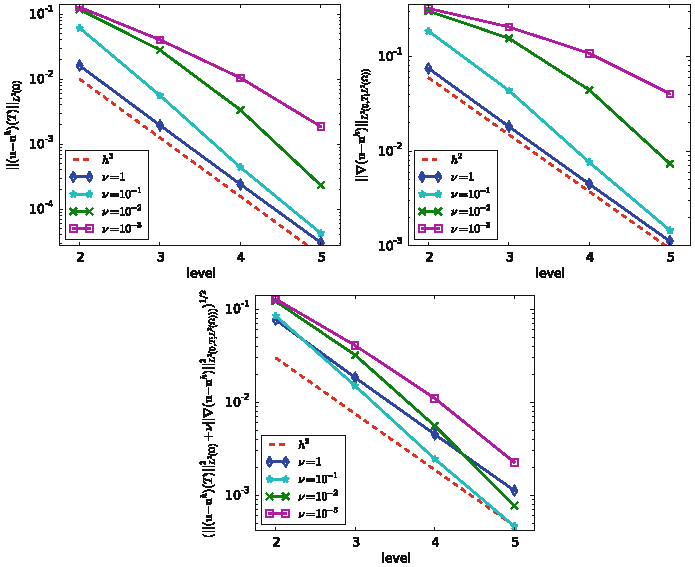
\includegraphics[width=\linewidth]{figures/Chapter_07/Fig_7_01__PDFp396__Bookp386.pdf}
  \captionof{figure}{例题 7.41:误差估计\hyperref[eq:time-dependent-fem-velocity-error]{(7.44)}左端两项误差及其和的收敛曲线.}
  \label{fig:time-dependent-error-convergence}
\end{elegantfigure}
\end{example}

\begin{theorem}[时间连续 Galerkin 有限元法的压力误差估计]
\label{thm:time-dependent-fem-pressure-error}
设定理\hyperref[thm:time-dependent-fem-velocity-error]{7.35} 的假设成立,并进一步假设
\begin{equation}\label{eq:time-dependent-fem-pressure-gradient-regularity}
  \nabla\bm{u}\in L^\infty(0,T;L^2(\Omega))
\end{equation}
且网格剖分族是拟一致的.则对所有 $t\in(0,T]$,有如下误差估计:
\begin{equation}\label{eq:time-dependent-fem-pressure-error}
\begin{aligned}
  \|p-p_h\|_{L^2(0,t;L^2(\Omega))}^2
  &\le C\left(1+\frac{1}{\beta_{\mathrm{is}}^h}\right)^2\\
  &\quad\cdot\inf_{q_h\in L^2(0,t;Q_h)}
       \|p-q_h\|_{L^2(0,t;L^2(\Omega))}^2\\
  &\quad+C\left(\frac{1}{\beta_{\mathrm{is}}^h}\right)^2
       \Bigl[
       \nu^2\|\nabla(\bm{u}-\bm{u}_h)\|_{L^2(0,t;L^2(\Omega))}^2\\
  &\qquad+\|\bm{u}-\bm{u}_h\|_{L^\infty(0,t;L^2(\Omega))}
       \|\nabla(\bm{u}-\bm{u}_h)\|_{L^2(0,t;L^2(\Omega))}\\
  &\qquad\quad\cdot\|\nabla\bm{u}\|_{L^4(0,t;L^2(\Omega))}^2\\
  &\qquad+\|\bm{u}_h\|_{L^\infty(0,t;L^2(\Omega))}
       \|\nabla\bm{u}_h\|_{L^\infty(0,t;L^2(\Omega))}\\
  &\qquad\quad\cdot\|\nabla(\bm{u}-\bm{u}_h)\|_{L^2(0,t;L^2(\Omega))}^2\\
  &\qquad+\|\partial_t(\bm{u}-I_h^{\mathrm{St}}\bm{u})\|_{L^2(0,t;V')}^2
       \Bigr].
\end{aligned}
\end{equation}
\end{theorem}

\begin{proof}
固定 $t\in(0,T]$.与定常问题的证明相同,先分解压力误差,再应用离散 inf-sup 条件\hyperref[eq:discrete-infsup-condition]{(3.51)};参见定理\hyperref[thm:steady-ns-fem-error-pressure]{6.30} 的证明.这样可得到与式\hyperref[eq:steady-ns-pressure-error-infsup]{(6.68)}同型的表达式,其分子为
\begin{equation}\label{eq:time-dependent-pressure-error-numerator}
\begin{aligned}
  &(\partial_t(\bm{u}-\bm{u}_h),\bm{v}_h)
  +\nu(\nabla(\bm{u}-\bm{u}_h),\nabla\bm{v}_h)\\
  &\quad+n_{\mathrm{skew}}(\bm{u},\bm{u},\bm{v}_h)
       -n_{\mathrm{skew}}(\bm{u}_h,\bm{u}_h,\bm{v}_h)
       -(\nabla\cdot\bm{v}_h,p-q_h).
\end{aligned}
\end{equation}

黏性项和含压力的项可像通常那样,利用对偶配对估计或 Cauchy--Schwarz 不等式\hyperref[eq:appendix-a-10]{(A.10)}以及估计\hyperref[eq:divergence-gradient-bound-h01]{(3.41)}得到
\begin{equation}\label{eq:time-dependent-pressure-error-viscous-bound}
  \nu\bigl|(\nabla(\bm{u}-\bm{u}_h),\nabla\bm{v}_h)\bigr|
  \le \nu\|\nabla(\bm{u}-\bm{u}_h)\|_{L^2(\Omega)}
       \|\nabla\bm{v}_h\|_{L^2(\Omega)},
\end{equation}
\begin{equation}\label{eq:time-dependent-pressure-error-pressure-bound}
  |(\nabla\cdot\bm{v}_h,p-q_h)|
  \le \|p-q_h\|_{L^2(\Omega)}
       \|\nabla\bm{v}_h\|_{L^2(\Omega)}.
\end{equation}
这两个估计中的第二个因子会与离散 inf-sup 条件分母中的相应因子约去.

接下来估计对流项.利用分解
\begin{equation}\label{eq:time-dependent-pressure-error-convection-splitting}
\begin{aligned}
  &n_{\mathrm{skew}}(\bm{u},\bm{u},\bm{v}_h)
   -n_{\mathrm{skew}}(\bm{u}_h,\bm{u}_h,\bm{v}_h)\\
  &=n_{\mathrm{skew}}(\bm{u}-\bm{u}_h,\bm{u},\bm{v}_h)
   +n_{\mathrm{skew}}(\bm{u}_h,\bm{u}-\bm{u}_h,\bm{v}_h).
\end{aligned}
\end{equation}
对第一项应用估计\hyperref[eq:steady-ns-conv-estimate-41]{(6.41)},取 $s=1/2$,可得
\begin{equation}\label{eq:time-dependent-pressure-error-convection-bound-1}
\begin{aligned}
  |n_{\mathrm{skew}}(\bm{u}-\bm{u}_h,\bm{u},\bm{v}_h)|
  \le{}&C\|\bm{u}-\bm{u}_h\|_{L^2(\Omega)}^{1/2}
       \|\nabla(\bm{u}-\bm{u}_h)\|_{L^2(\Omega)}^{1/2}\\
  &\quad\cdot\|\nabla\bm{u}\|_{L^2(\Omega)}
       \|\nabla\bm{v}_h\|_{L^2(\Omega)}.
\end{aligned}
\end{equation}
最后一个因子同样与离散 inf-sup 条件分母中的相应因子约去.为估计 $L^2(0,t;L^2(\Omega))$ 范数下的压力误差,还需将其余各项平方并对时间积分.由 Cauchy--Schwarz 不等式,
\[
\begin{aligned}
  &\int_0^t
       \|\bm{u}-\bm{u}_h\|_{L^2(\Omega)}
       \|\nabla(\bm{u}-\bm{u}_h)\|_{L^2(\Omega)}
       \|\nabla\bm{u}\|_{L^2(\Omega)}^2\,\mathrm{d}\tau\\
  &\quad\le
       \|\bm{u}-\bm{u}_h\|_{L^\infty(0,t;L^2(\Omega))}
       \|\nabla(\bm{u}-\bm{u}_h)\|_{L^2(0,t;L^2(\Omega))}
       \|\nabla\bm{u}\|_{L^4(0,t;L^2(\Omega))}^2.
\end{aligned}
\]
其中前两个因子由估计\hyperref[eq:time-dependent-fem-velocity-error]{(7.44)}控制,第三个因子则由假设\hyperref[eq:time-dependent-fem-error-regularity]{(7.43)}控制.

對式\hyperref[eq:time-dependent-pressure-error-convection-splitting]{(7.64)}中的第二項同樣處理,可得
\begin{equation}\label{eq:time-dependent-pressure-error-convection-bound-2}
\begin{aligned}
  |n_{\mathrm{skew}}(\bm{u}_h,\bm{u}-\bm{u}_h,\bm{v}_h)|
  \le{}&C\|\bm{u}_h\|_{L^2(\Omega)}^{1/2}
       \|\nabla\bm{u}_h\|_{L^2(\Omega)}^{1/2}\\
  &\quad\cdot\|\nabla(\bm{u}-\bm{u}_h)\|_{L^2(\Omega)}
       \|\nabla\bm{v}_h\|_{L^2(\Omega)}.
\end{aligned}
\end{equation}
约去 $\|\nabla\bm{v}_h\|_{L^2(\Omega)}$,再平方并在 $(0,t)$ 上积分,得到
\[
\begin{aligned}
  &\int_0^t
       \|\bm{u}_h\|_{L^2(\Omega)}
       \|\nabla\bm{u}_h\|_{L^2(\Omega)}
       \|\nabla(\bm{u}-\bm{u}_h)\|_{L^2(\Omega)}^2\,\mathrm{d}\tau\\
  &\quad\le
       \|\bm{u}_h\|_{L^\infty(0,t;L^2(\Omega))}
       \|\nabla\bm{u}_h\|_{L^\infty(0,t;L^2(\Omega))}
       \|\nabla(\bm{u}-\bm{u}_h)\|_{L^2(0,t;L^2(\Omega))}^2.
\end{aligned}
\]
第一个因子由稳定性估计\hyperref[eq:time-dependent-fem-velocity-stability]{(7.42)}控制.对时刻 $t$ 的 Stokes 投影 $I_h^{\mathrm{St}}\bm{u}$ 应用三角不等式、估计\hyperref[eq:stokes-projection-best-approximation-velocity]{(4.57)}和逆估计\hyperref[eq:appendix-c-35]{(C.35)},并沿用定理\hyperref[thm:time-dependent-fem-velocity-error]{7.35} 证明中的记号,有
\begin{equation}\label{eq:time-dependent-pressure-error-discrete-gradient-bound}
\begin{aligned}
  \|\nabla\bm{u}_h\|_{L^2(\Omega)}
  &\le \|\nabla(\bm{u}-I_h^{\mathrm{St}}\bm{u})\|_{L^2(\Omega)}
       +\|\nabla(I_h^{\mathrm{St}}\bm{u}-\bm{u}_h)\|_{L^2(\Omega)}
       +\|\nabla\bm{u}\|_{L^2(\Omega)}\\
  &\le C\|\nabla\bm{u}\|_{L^2(\Omega)}
       +Ch^{-1}\|I_h^{\mathrm{St}}\bm{u}-\bm{u}_h\|_{L^2(\Omega)}
       +\|\nabla\bm{u}\|_{L^2(\Omega)}\\
  &=C\|\nabla\bm{u}\|_{L^2(\Omega)}\\
  &+Ch^{-1}\|\symbf{\phi}_h\|_{L^2(\Omega)}.
\end{aligned}
\end{equation}
这里 $\symbf{\phi}_h=\bm{u}_h-I_h^{\mathrm{St}}\bm{u}$.由估计\hyperref[eq:time-dependent-fem-error-gronwall]{(7.56)},第二项在 $L^\infty(0,t;L^2(\Omega))$ 中有界;若收敛阶至少为一阶,则 $h^{-1}$ 的负幂可由误差中的 $h$ 阶收敛补偿.对式\hyperref[eq:time-dependent-pressure-error-discrete-gradient-bound]{(7.67)}右端的另一项,则需假设\hyperref[eq:time-dependent-fem-pressure-gradient-regularity]{(7.59)}.在这一假设下,式\hyperref[eq:time-dependent-pressure-error-convection-splitting]{(7.64)}中的第二项也可得到控制.

现在分析式\hyperref[eq:time-dependent-pressure-error-numerator]{(7.61)}中的时间导数项.先将它分解为
\[
\begin{aligned}
  (\partial_t(\bm{u}-\bm{u}_h),\bm{v}_h)
  ={}&(\partial_t(\bm{u}-I_h^{\mathrm{St}}\bm{u}),\bm{v}_h)\\
  &+(\partial_t(I_h^{\mathrm{St}}\bm{u}-\bm{u}_h),\bm{v}_h).
\end{aligned}
\]
第一项利用对偶配对估计可得
\begin{equation}\label{eq:time-dependent-pressure-error-time-derivative-projection}
  |(\partial_t(\bm{u}-I_h^{\mathrm{St}}\bm{u}),\bm{v}_h)|
  \le \|\partial_t(\bm{u}-I_h^{\mathrm{St}}\bm{u})\|_{V'}
       \|\nabla\bm{v}_h\|_{L^2(\Omega)}.
\end{equation}
对另一项作同样处理,并沿用定理\hyperref[thm:time-dependent-fem-velocity-error]{7.35} 证明中的记号,得到
\begin{equation}\label{eq:time-dependent-pressure-error-time-derivative-discrete}
  |(\partial_t(I_h^{\mathrm{St}}\bm{u}-\bm{u}_h),\bm{v}_h)|
  \le \|\partial_t\symbf{\phi}_h\|_{V'}
       \|\nabla\bm{v}_h\|_{L^2(\Omega)}.
\end{equation}

为估计式\hyperref[eq:time-dependent-pressure-error-time-derivative-discrete]{(7.69)}中的第一因子,引入离散 Stokes 算子 $A_h:V_{\mathrm{div}}^h\to V_{\mathrm{div}}^h$,其定义为
\begin{equation}\label{eq:time-dependent-pressure-error-discrete-stokes-operator}
  (A_h\bm{v}_h,\bm{w}_h)
  =(\nabla\bm{v}_h,\nabla\bm{w}_h)
  \qquad\forall\,\bm{v}_h,\bm{w}_h\in V_{\mathrm{div}}^h.
\end{equation}
算子 $A_h$ 对称(自伴)且正定.在式\hyperref[eq:time-dependent-pressure-error-discrete-stokes-operator]{(7.70)}中取 $\bm{w}_h=\bm{v}_h$,可得
\begin{equation}\label{eq:time-dependent-pressure-error-discrete-stokes-norm}
\begin{aligned}
  \|\nabla\bm{v}_h\|_{L^2(\Omega)}
  &=(A_h\bm{v}_h,\bm{v}_h)^{1/2}\\
  &=((A_h)^{1/2}\bm{v}_h,(A_h)^{1/2}\bm{v}_h)^{1/2}
   =\|(A_h)^{1/2}\bm{v}_h\|_{L^2(\Omega)}.
\end{aligned}
\end{equation}
再在式\hyperref[eq:time-dependent-pressure-error-discrete-stokes-operator]{(7.70)}中令两个自变量都等于 $(A_h)^{-1/2}\bm{v}_h$,得到
\begin{equation}\label{eq:time-dependent-pressure-error-discrete-stokes-negative-norm}
  \|\nabla(A_h)^{-1/2}\bm{v}_h\|_{L^2(\Omega)}
  =\|\bm{v}_h\|_{L^2(\Omega)}.
\end{equation}

由 \textcite{AyusoGarciaArchillaNovo2005}(引理 3.11 及式(2.15))可得估计
\[
  \|\partial_t\symbf{\phi}_h\|_{V'}
  \le Ch\|\partial_t\symbf{\phi}_h\|_{L^2(\Omega)}
       +C\|(A_h)^{-1/2}\partial_t\symbf{\phi}_h\|_{L^2(\Omega)}.
\]
右端第一项可由式\hyperref[eq:time-dependent-pressure-error-discrete-stokes-norm]{(7.71)}和逆估计\hyperref[eq:appendix-c-35]{(C.35)}控制:
\[
\begin{aligned}
  Ch\|\partial_t\symbf{\phi}_h\|_{L^2(\Omega)}
  &=Ch\|A_h^{1/2}A_h^{-1/2}
       \partial_t\symbf{\phi}_h\|_{L^2(\Omega)}\\
  &=Ch\|\nabla A_h^{-1/2}
       \partial_t\symbf{\phi}_h\|_{L^2(\Omega)}
   \le C\|A_h^{-1/2}\partial_t\symbf{\phi}_h\|_{L^2(\Omega)}.
\end{aligned}
\]
因此,
\begin{equation}\label{eq:time-dependent-pressure-error-time-derivative-negative-norm}
  \|\partial_t\symbf{\phi}_h\|_{V'}
  \le C\|(A_h)^{-1/2}\partial_t\symbf{\phi}_h\|_{L^2(\Omega)}.
\end{equation}

为控制式\hyperref[eq:time-dependent-pressure-error-time-derivative-negative-norm]{(7.73)}右端,取误差方程\hyperref[eq:time-dependent-fem-error-equation]{(7.48)}中的检验函数
$\bm{v}_h=A_h^{-1}\partial_t\symbf{\phi}_h\in V_{\mathrm{div}}^h$.逐项估计可得
\begin{equation}\label{eq:time-dependent-pressure-error-time-derivative-test}
\begin{aligned}
  (\partial_t\symbf{\phi}_h,
       A_h^{-1}\partial_t\symbf{\phi}_h)
  &=(A_h^{-1/2}\partial_t\symbf{\phi}_h,
       A_h^{-1/2}\partial_t\symbf{\phi}_h)\\
  &=\|A_h^{-1/2}\partial_t\symbf{\phi}_h\|_{L^2(\Omega)}^2.
\end{aligned}
\end{equation}
利用对偶配对估计和式\hyperref[eq:time-dependent-pressure-error-discrete-stokes-negative-norm]{(7.72)},有
\begin{equation}\label{eq:time-dependent-pressure-error-time-derivative-projection-test}
\begin{aligned}
  |(\partial_t\symbf{\eta},A_h^{-1}\partial_t\symbf{\phi}_h)|
  &\le \|\partial_t\symbf{\eta}\|_{V'}
       \|\nabla(A_h^{-1}\partial_t\symbf{\phi}_h)\|_{L^2(\Omega)}\\
  &=\|\partial_t(\bm{u}-I_h^{\mathrm{St}}\bm{u})\|_{V'}
       \|A_h^{-1/2}\partial_t\symbf{\phi}_h\|_{L^2(\Omega)}.
\end{aligned}
\end{equation}
利用离散 Stokes 算子的定义、Cauchy--Schwarz 不等式和式\hyperref[eq:time-dependent-pressure-error-discrete-stokes-norm]{(7.71)},黏性项满足
\begin{equation}\label{eq:time-dependent-pressure-error-viscous-test}
\begin{aligned}
  &\nu\bigl|(\nabla(\bm{u}-\bm{u}_h),
       \nabla(A_h^{-1}\partial_t\symbf{\phi}_h))\bigr|\\
  &\quad\le \nu\|\nabla(\bm{u}-\bm{u}_h)\|_{L^2(\Omega)}
       \|A_h^{-1/2}\partial_t\symbf{\phi}_h\|_{L^2(\Omega)}.
\end{aligned}
\end{equation}
对压力项应用 Cauchy--Schwarz 不等式、式\hyperref[eq:divergence-gradient-bound-h01]{(3.41)}和\hyperref[eq:time-dependent-pressure-error-discrete-stokes-negative-norm]{(7.72)},并按式\hyperref[eq:time-dependent-pressure-error-time-derivative-projection-test]{(7.75)}处理检验函数项,得到
\begin{equation}\label{eq:time-dependent-pressure-error-pressure-test}
\begin{aligned}
  |(\nabla\cdot(A_h^{-1}\partial_t\symbf{\phi}_h),p-q_h)|
  &\le \|p-q_h\|_{L^2(\Omega)}
       \|\nabla(A_h^{-1}\partial_t\symbf{\phi}_h)\|_{L^2(\Omega)}\\
  &=\|p-q_h\|_{L^2(\Omega)}
       \|A_h^{-1/2}\partial_t\symbf{\phi}_h\|_{L^2(\Omega)}.
\end{aligned}
\end{equation}
对非线性项采用推导估计\hyperref[eq:time-dependent-pressure-error-convection-bound-1]{(7.65)}和\hyperref[eq:time-dependent-pressure-error-convection-bound-2]{(7.66)}时的相同方法,并按式\hyperref[eq:time-dependent-pressure-error-time-derivative-projection-test]{(7.75)}处理检验函数,得到
\begin{equation}\label{eq:time-dependent-pressure-error-convection-test}
\begin{aligned}
  &\bigl|n_{\mathrm{skew}}(\bm{u},\bm{u},
       A_h^{-1}\partial_t\symbf{\phi}_h)
       -n_{\mathrm{skew}}(\bm{u}_h,\bm{u}_h,
       A_h^{-1}\partial_t\symbf{\phi}_h)\bigr|\\
  &\quad\le C\Bigl(
       \|\bm{u}-\bm{u}_h\|_{L^2(\Omega)}^{1/2}
       \|\nabla(\bm{u}-\bm{u}_h)\|_{L^2(\Omega)}^{1/2}
       \|\nabla\bm{u}\|_{L^2(\Omega)}\\
  &\qquad\quad+
       \|\bm{u}_h\|_{L^2(\Omega)}^{1/2}
       \|\nabla\bm{u}_h\|_{L^2(\Omega)}^{1/2}
       \|\nabla(\bm{u}-\bm{u}_h)\|_{L^2(\Omega)}
       \Bigr)\\
  &\qquad\cdot\|A_h^{-1/2}\partial_t\symbf{\phi}_h\|_{L^2(\Omega)}.
\end{aligned}
\end{equation}
式\hyperref[eq:time-dependent-pressure-error-time-derivative-projection-test]{(7.75)}至\hyperref[eq:time-dependent-pressure-error-convection-test]{(7.78)}各式右端的第二个因子,可与式\hyperref[eq:time-dependent-pressure-error-time-derivative-test]{(7.74)}中的一个因子约去,从而得到 $\|A_h^{-1/2}\partial_t\symbf{\phi}_h\|_{L^2(\Omega)}$ 的上界.该上界只含有已出现在估计\hyperref[eq:time-dependent-pressure-error-viscous-bound]{(7.62)}、\hyperref[eq:time-dependent-pressure-error-pressure-bound]{(7.63)}、\hyperref[eq:time-dependent-pressure-error-convection-bound-1]{(7.65)}、\hyperref[eq:time-dependent-pressure-error-convection-bound-2]{(7.66)}和\hyperref[eq:time-dependent-pressure-error-time-derivative-projection]{(7.68)}中的项.将其代入式\hyperref[eq:time-dependent-pressure-error-time-derivative-negative-norm]{(7.73)},再代入式\hyperref[eq:time-dependent-pressure-error-time-derivative-discrete]{(7.69)},便完成了对时间导数项的估计.总的来说,该估计所引入的各项与式\hyperref[eq:time-dependent-pressure-error-numerator]{(7.61)}其他项的估计中已有的项相同.

汇总估计\hyperref[eq:time-dependent-pressure-error-viscous-bound]{(7.62)}、\hyperref[eq:time-dependent-pressure-error-pressure-bound]{(7.63)}、\hyperref[eq:time-dependent-pressure-error-convection-bound-1]{(7.65)}、\hyperref[eq:time-dependent-pressure-error-convection-bound-2]{(7.66)}、\hyperref[eq:time-dependent-pressure-error-time-derivative-projection]{(7.68)}和\hyperref[eq:time-dependent-pressure-error-time-derivative-discrete]{(7.69)},对所有 $q_h\in Q_h$ 有
\begin{equation}\label{eq:time-dependent-pressure-error-pointwise}
\begin{aligned}
  \|p_h-q_h\|_{L^2(\Omega)}
  \le \frac{C}{\beta_{\mathrm{is}}^h}\Bigl[{}
       &\nu\|\nabla(\bm{u}-\bm{u}_h)\|_{L^2(\Omega)}\\
       &+\|\bm{u}-\bm{u}_h\|_{L^2(\Omega)}^{1/2}
        \|\nabla(\bm{u}-\bm{u}_h)\|_{L^2(\Omega)}^{1/2}
        \|\nabla\bm{u}\|_{L^2(\Omega)}\\
       &+\|\bm{u}_h\|_{L^2(\Omega)}^{1/2}
        \|\nabla\bm{u}_h\|_{L^2(\Omega)}^{1/2}
        \|\nabla(\bm{u}-\bm{u}_h)\|_{L^2(\Omega)}\\
       &+\|\partial_t(\bm{u}-I_h^{\mathrm{St}}\bm{u})\|_{V'}
        +\|p-q_h\|_{L^2(\Omega)}\Bigr].
\end{aligned}
\end{equation}
最后应用三角不等式
$\|p-p_h\|_{L^2(\Omega)}\le\|p-q_h\|_{L^2(\Omega)}+\|p_h-q_h\|_{L^2(\Omega)}$,代入估计\hyperref[eq:time-dependent-pressure-error-pointwise]{(7.79)},将两边平方并在 $(0,t)$ 上积分,即得压力误差估计\hyperref[eq:time-dependent-fem-pressure-error]{(7.60)}.
\end{proof}

\begin{note}[关于误差估计(7.60)]
\label{note:time-dependent-fem-pressure-error-interpretation}
误差估计\hyperref[eq:time-dependent-fem-pressure-error]{(7.60)}右端含有已由速度误差估计\hyperref[eq:time-dependent-fem-velocity-error]{(7.44)}控制的速度误差,以及该速度误差估计右端出现的项.因此,压力误差 $\|p-p_h\|_{L^2(0,t;L^2(\Omega))}$ 的收敛阶与式\hyperref[eq:time-dependent-fem-velocity-error]{(7.44)}左端速度误差的收敛阶相同.
\end{note}

\begin{example}[解析解对误差估计(7.60)的数值验证]
\label{ex:time-dependent-pressure-error}
采用例题\hyperref[ex:appendix-d-7]{D.7}中的 $Q_2/P_1^{\mathrm{disc}}$ 有限元空间对进行数值模拟.初始网格(层级 0)为图\hyperref[fig:stokes-example-initial-grids]{4.2}所示的不规则四边形网格.时间离散采用 Crank--Nicolson 格式,时间步长均匀取 $\Delta t=10^{-4}$,终止时刻为 $T=5$.

压力误差的计算结果见图\hyperref[fig:time-dependent-pressure-error-convergence]{7.2}.可以清楚地观察到二阶收敛.在本例中,压力误差不依赖于黏度.
\end{example}

\begin{note}[平均量的数值分析]
\label{note:time-dependent-fem-averaged-quantities}
在许多应用中,时间平均量或时空平均量都很重要.然而,到目前为止,关于这些量的数值分析结果仍然很少;例如可参见 \textcite{JohnLaytonManica2007}.
\end{note}

\begin{elegantfigure}[0.64\linewidth]
  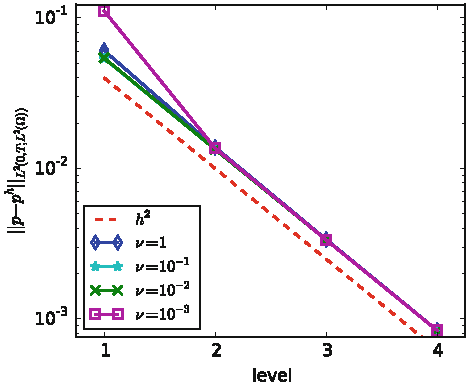
\includegraphics[width=\linewidth]{figures/Chapter_07/Fig_7_02__PDFp403__Bookp393.pdf}
  \captionof{figure}{例题 7.44:压力误差的收敛曲线.}
  \label{fig:time-dependent-pressure-error-convergence}
\end{elegantfigure}

\section{导致耦合问题的时间离散}
\label{sec:time-discretizations-coupled-problems}

\subsection{\texorpdfstring{$\theta$}{θ}-格式作为时间离散方法}
\label{subsec:theta-schemes}

\begin{note}[$\theta$-格式的基本应用思路]
\label{note:theta-scheme-principal-approach}
为完全离散并线性化方程组\hyperref[eq:time-dependent-ns-strong]{(7.1)},$\theta$-格式采用以下步骤:
\begin{enumerate}
  \item 对方程组\hyperref[eq:time-dependent-ns-strong]{(7.1)}作时间半离散.时间半离散后,在每个离散时刻都得到一个非线性鞍点型方程组.
  \item 写出变分形式并作线性化.将非线性方程组改写为变分问题,再将非线性变分问题线性化.
  \item 对线性系统作空间离散.求解非线性问题的迭代过程中,每一步都会产生一个线性系统;随后用有限元方法对该系统作空间离散,例如选用满足 inf-sup 条件的有限元空间对.
\end{enumerate}
这种方法先离散时间、再离散空间,也称为 Rothe 方法或水平线法.各步骤将在本节中详细说明.另一种方法先作空间离散以得到常微分方程组,再对时间离散,称为垂直线法.
\index{theta-format@$\theta$-格式}\index{Rothe method@Rothe 方法}\index{horizontal-lines-method@水平线法}\index{vertical-lines-method@垂直线法}
\end{note}

\begin{note}[记号约定]
\label{note:time-discretization-notation}
设 $t_n\in[0,T]$.在离散时刻 $t_n$ 取值的量用下标 $n$ 表示.从离散时刻 $t_n$ 到下一个离散时刻 $t_{n+1}$ 的时间步长记为 $\Delta t_{n+1}$,即
\[
  \Delta t_{n+1}=t_{n+1}-t_n.
\]
\end{note}

\begin{note}[Navier--Stokes 方程的单步 $\theta$-格式]
\label{note:one-step-theta-scheme}
取 $\theta\in[0,1]$,考察从 $t_n$ 到 $t_{n+1}$ 的时间步.Navier--Stokes 方程的单步 $\theta$-格式可写为
\begin{equation}\label{eq:theta-scheme-one-step}
\begin{aligned}
  \frac{\bm{u}_{n+1}}{\Delta t_{n+1}}
  &+\theta\Bigl[-\nu\Delta\bm{u}_{n+1}
       +(\bm{u}_{n+1}\cdot\nabla)\bm{u}_{n+1}\Bigr]\\
  &+\nabla p_{n+1}
       =\frac{\bm{u}_n}{\Delta t_{n+1}}\\
  &\quad-(1-\theta)\Bigl[-\nu\Delta\bm{u}_n\\
  &\qquad+(\bm{u}_n\cdot\nabla)\bm{u}_n\Bigr]\\
  &\quad+(1-\theta)\bm{f}_n+\theta\bm{f}_{n+1},\\
  0&=\nabla\cdot\bm{u}_{n+1}.
\end{aligned}
\end{equation}
\end{note}

\begin{example}[显式与隐式 Euler 格式、Crank--Nicolson 格式]
\label{ex:time-dependent-crank-nicolson}
三个常用的单步 $\theta$-格式——前向与后向 Euler 格式以及 Crank--Nicolson 格式——由 $\theta$ 的相应取值给出:
\begin{itemize}
  \item $\theta=0$:前向(显式)Euler 格式;
  \item $\theta=0.5$:Crank--Nicolson 格式;
  \item $\theta=1$:后向(隐式)Euler 格式.
\end{itemize}
\index{explicit-Euler@前向 Euler 格式}\index{implicit-Euler@后向 Euler 格式}\index{Crank-Nicolson@Crank--Nicolson 格式}
关于这些格式,还有几点值得说明.更详细的讨论将在数值算例之后的笔记\hyperref[note:theta-scheme-comments]{7.59} 中给出.
\begin{itemize}
  \item \textit{前向或显式 Euler 格式.}黏性项与扩散项形式相同,会使时间方向上的常微分方程组成为刚性问题;参见 \textcite{HairerWanner2010}(第 6 页).常微分方程数值分析表明,对刚性问题,为获得稳定模拟,显式格式必须采用很小的时间步长.对于 Navier--Stokes 方程,时间步长通常小到使模拟效率很低.因此,不建议用前向 Euler 格式或其他显式格式离散不可压缩 Navier--Stokes 方程.
  \item \textit{后向或隐式 Euler 格式.}这是一阶格式,应用相当广泛.不过,文献中已有研究指出,参见 \textcite{JohnMatthiesRang2006a};例题\hyperref[ex:time-dependent-accuracy-comparison]{7.58} 也将说明,将后向 Euler 格式与高阶空间离散结合时,所得结果可能比采用高阶时间离散时的结果精度差得多.
  \item \textit{Crank--Nicolson 格式(梯形公式).}Crank--Nicolson 格式是二阶格式,应用非常普遍.
  \item \textit{一般情形.}对于时间变化的自适应网格,\textcite{BesierWollner2012} 观察并分析了单步格式中压力近似的缺陷.该文研究了若干处理方案,最终认为,最佳做法是在网格改变后的至少一个时间步中采用例题\hyperref[ex:fractional-step-theta-scheme]{7.52} 所述的分步 $\theta$-格式.
\end{itemize}
\end{example}

\begin{note}[关于不可压缩约束]
\label{note:theta-scheme-incompressibility}
\begin{itemize}
  \item 式\hyperref[eq:theta-scheme-one-step]{(7.80)}中的时间导数是在 $t_n+\theta\Delta t_{n+1}$ 处近似的;参见式\hyperref[eq:midpoint-difference-consistency]{(7.94)}.因此,速度也近似于这一时刻的值,而压力则是该速度对应的拉格朗日乘子.例如,在 Crank--Nicolson 格式下,计算所得解近似于 $(\bm{u}_{n+1/2},p_{n+1/2})$.若希望在时刻 $t_{n+1}$ 得到较准确的压力近似,则可将 Crank--Nicolson 格式中的压力项改为
  \[
    \frac12(p_{n+1}+p_n),
  \]
  例如参见 \textcite{Rang2008}.不过,该格式在第一步中需要初始时刻的压力;关于这一问题,见笔记\hyperref[note:time-dependent-initial-pressure]{7.29}.

  \item 与 Stokes 方程的式\hyperref[eq:stokes-abstract-weak]{(4.3)}类似,时间步\hyperref[eq:theta-scheme-one-step]{(7.80)}的变分形式可在乘积空间中写出:求 $(\bm{u}_{n+1},p_{n+1})\in V\times Q$,使得对所有 $(\bm{v},q)\in V\times Q$,
  \[
  \begin{aligned}
    \frac{1}{\Delta t_{n+1}}(\bm{u}_{n+1},\bm{v})
    &+\theta\Bigl[\nu(\nabla\bm{u}_{n+1},\nabla\bm{v})
       +((\bm{u}_{n+1}\cdot\nabla)\bm{u}_{n+1},\bm{v})\Bigr]\\
    &+(\nabla\cdot\bm{u}_{n+1},q)
       -(\nabla\cdot\bm{v},p_{n+1})\\
    &=\frac{1}{\Delta t_{n+1}}(\bm{u}_n,\bm{v})\\
    &\quad-(1-\theta)\Bigl[\nu(\nabla\bm{u}_n,\nabla\bm{v})
       +((\bm{u}_n\cdot\nabla)\bm{u}_n,\bm{v})\Bigr]\\
    &\quad+(1-\theta)\langle\bm{f}_n,\bm{v}\rangle_{V',V}
       +\theta\langle\bm{f}_{n+1},\bm{v}\rangle_{V',V}.
  \end{aligned}
  \]
  等价地,将整个问题乘以 $\Delta t_{n+1}$ 后,可得
  \begin{equation}\label{eq:theta-scheme-variational}
  \begin{aligned}
    &(\bm{u}_{n+1},\bm{v})
      +\theta\Delta t_{n+1}\Bigl[\nu(\nabla\bm{u}_{n+1},\nabla\bm{v})
       +((\bm{u}_{n+1}\cdot\nabla)\bm{u}_{n+1},\bm{v})\Bigr]\\
    &\quad+\Delta t_{n+1}(\nabla\cdot\bm{u}_{n+1},q)
       -\Delta t_{n+1}(\nabla\cdot\bm{v},p_{n+1})\\
    &=(\bm{u}_n,\bm{v})
       -(1-\theta)\Delta t_{n+1}\Bigl[\nu(\nabla\bm{u}_n,\nabla\bm{v})
       +((\bm{u}_n\cdot\nabla)\bm{u}_n,\bm{v})\Bigr]\\
    &\quad+(1-\theta)\Delta t_{n+1}\langle\bm{f}_n,\bm{v}\rangle_{V',V}
       +\theta\Delta t_{n+1}\langle\bm{f}_{n+1},\bm{v}\rangle_{V',V}.
  \end{aligned}
  \end{equation}
  在式\hyperref[eq:theta-scheme-variational]{(7.81)}中取 $(\bm{v},q)=(\bm{u},p)$,可见散度项相消.这与定常问题的分析相同,例如引理\hyperref[lem:steady-ns-stability]{6.21} 的证明.因此,就这一点而言,式\hyperref[eq:theta-scheme-variational]{(7.81)}具有与定常问题变分形式相同的性质.

  相应的式\hyperref[eq:theta-scheme-variational]{(7.81)}强形式为
  \begin{equation}\label{eq:theta-scheme-strong}
  \begin{aligned}
    \bm{u}_{n+1}
    &+\theta\Delta t_{n+1}\Bigl[-\nu\Delta\bm{u}_{n+1}\\
    &\quad+(\bm{u}_{n+1}\cdot\nabla)\bm{u}_{n+1}\Bigr]\\
    &+\Delta t_{n+1}\nabla p_{n+1}=\bm{u}_n\\
    &\quad-(1-\theta)\Delta t_{n+1}\Bigl[-\nu\Delta\bm{u}_n\\
    &\qquad+(\bm{u}_n\cdot\nabla)\bm{u}_n\Bigr]\\
    &\quad+(1-\theta)\Delta t_{n+1}\bm{f}_n
       +\theta\Delta t_{n+1}\bm{f}_{n+1},\\
    0&=\Delta t_{n+1}\nabla\cdot\bm{u}_{n+1}.
  \end{aligned}
  \end{equation}
  可见,散度约束乘上了 $\Delta t_{n+1}$.当然,也可以只将式\hyperref[eq:theta-scheme-one-step]{(7.80)}中的动量方程乘以 $\Delta t_{n+1}$,而保持连续性方程不变;这样得到的问题在数学上与式\hyperref[eq:theta-scheme-variational]{(7.81)}等价.除这一注记中给出的缩放理由外,根据我们的经验,对含缩放散度约束的问题\hyperref[eq:theta-scheme-variational]{(7.81)}作数值求解效率更高.本专著所列所有含时问题的模拟,均按式\hyperref[eq:theta-scheme-variational]{(7.81)}或\hyperref[eq:theta-scheme-strong]{(7.82)}对散度约束作了时间步长缩放.
\end{itemize}
\end{note}

\begin{note}[Navier--Stokes 方程的一般 $\theta$-格式]
\label{note:general-theta-scheme}
Navier--Stokes 方程组\hyperref[eq:time-dependent-ns-strong]{(7.1)}的一般 $\theta$-格式在某个时间步中的形式为
\begin{equation}\label{eq:general-theta-scheme}
\begin{aligned}
  \frac{\bm{u}_{k+1}}{\Delta t_{n+1}}
  &+\theta_1\Bigl[-\nu\Delta\bm{u}_{k+1}
       +(\bm{u}_{k+1}\cdot\nabla)\bm{u}_{k+1}\Bigr]\\
  &+\frac{\Delta t_{k+1}}{\Delta t_{n+1}}\nabla p_{k+1}
       =\frac{\bm{u}_k}{\Delta t_{n+1}}\\
  &\quad-\theta_2\Bigl[-\nu\Delta\bm{u}_k\\
  &\qquad+(\bm{u}_k\cdot\nabla)\bm{u}_k\Bigr]
       +\theta_3\bm{f}_k+\theta_4\bm{f}_{k+1},\\
  0&=\Delta t_{k+1}\nabla\cdot\bm{u}_{k+1},
\end{aligned}
\end{equation}
其中参数为 $\theta_1,\ldots,\theta_4$.注意,时间指标 $k$ 与 $n$ 不同.
\end{note}

\begin{example}[分步 $\theta$-格式]
\label{ex:fractional-step-theta-scheme}
\textcite{BristeauGlowinskiPeriaux1987} 提出的分步 $\theta$-格式由三个式\hyperref[eq:general-theta-scheme]{(7.83)}形式的步骤组成.该格式有 FS0 和 FS1 两个变体,列于表\hyperref[tab:fractional-step-theta-variants]{7.1}.其中
\[
  \theta=1-\frac{\sqrt{2}}{2},\qquad
  \widetilde{\theta}=1-2\theta,\qquad
  \tau=\frac{\widetilde{\theta}}{1-\theta},\qquad
  \eta=1-\tau.
\]
\index{fractional-step-theta@分步 $\theta$-格式}
分步 $\theta$-格式巧妙地组合了三个一阶单步格式,从而得到强 A-稳定的二阶格式.FS1 只需在 $t_n$ 和 $t_{n+1}-\theta\Delta t_{n+1}$ 处计算 $\bm{f}$;FS0 还需额外在 $t_n+\theta\Delta t_{n+1}$ 和 $t_{n+1}$ 处计算.两种变体都是二阶格式,但 FS1 对关于时间 $t$ 的二次多项式不能精确积分.在稳定性等其他基本性质方面,两者大致相同.关于二维 Navier--Stokes 方程的数值结果,\textcite{JohnMatthiesRang2006a} 表明 FS0 通常比 FS1 精确得多.因此,若计算右端项的代价不高,应优先采用 FS0.

\begin{eleganttable}
\centering
\captionof{table}{分步 $\theta$-格式的两个变体}
\label{tab:fractional-step-theta-variants}
\scriptsize
\setlength{\tabcolsep}{2.5pt}
\renewcommand{\arraystretch}{1.16}
\resizebox{\linewidth}{!}{%
\begin{tabular}{c|cccc|cc|c|c}
\hline
 & $\theta_1$ & $\theta_2$ & $\theta_3$ & $\theta_4$
 & $t_k$ & $t_{k+1}$ & $\Delta t_{k+1}$ & 阶数 \\
\hline
FS0 & $\tau\theta$ & $\eta\theta$ & $\eta\theta$ & $\tau\theta$
    & $t_n$ & $t_n+\theta\Delta t_{n+1}$ & $\theta\Delta t_{n+1}$ & 2 \\
    & $\eta\widetilde{\theta}$ & $\tau\widetilde{\theta}$
    & $\tau\widetilde{\theta}$ & $\eta\widetilde{\theta}$
    & $t_n+\theta\Delta t_{n+1}$ & $t_{n+1}-\theta\Delta t_{n+1}$
    & $\widetilde{\theta}\Delta t_{n+1}$ & \\
    & $\tau\theta$ & $\eta\theta$ & $\eta\theta$ & $\tau\theta$
    & $t_{n+1}-\theta\Delta t_{n+1}$ & $t_{n+1}$
    & $\theta\Delta t_{n+1}$ & \\
\hline
FS1 & $\tau\theta$ & $\eta\theta$ & $\theta$ & $0$
    & $t_n$ & $t_n+\theta\Delta t_{n+1}$ & $\theta\Delta t_{n+1}$ & 2 \\
    & $\eta\widetilde{\theta}$ & $\tau\widetilde{\theta}$
    & $0$ & $\widetilde{\theta}$
    & $t_n+\theta\Delta t_{n+1}$ & $t_{n+1}-\theta\Delta t_{n+1}$
    & $\widetilde{\theta}\Delta t_{n+1}$ & \\
    & $\tau\theta$ & $\eta\theta$ & $\theta$ & $0$
    & $t_{n+1}-\theta\Delta t_{n+1}$ & $t_{n+1}$
    & $\theta\Delta t_{n+1}$ & \\
\hline
\end{tabular}%
}
\end{eleganttable}
\end{example}

\begin{note}[$\theta$-格式的统一表示]
\label{note:theta-scheme-comments}
注意,单步 $\theta$-格式\hyperref[eq:theta-scheme-one-step]{(7.80)}在参数取适当值时,可写成一般 $\theta$-格式\hyperref[eq:general-theta-scheme]{(7.83)};见表\hyperref[tab:one-step-theta-parameters]{7.2}.因此,式\hyperref[eq:general-theta-scheme]{(7.83)}使所有已介绍格式都能用同一个公式实现,并可通过设置四个参数来选择具体格式.本节之后关于 $\theta$-格式的讨论,都将采用一般 $\theta$-格式\hyperref[eq:general-theta-scheme]{(7.83)}.

\begin{eleganttable}
\centering
\captionof{table}{写成一般 $\theta$-格式(7.83)时单步 $\theta$-格式的参数}
\label{tab:one-step-theta-parameters}
\scriptsize
\setlength{\tabcolsep}{3pt}
\renewcommand{\arraystretch}{1.18}
\resizebox{\linewidth}{!}{%
\begin{tabular}{l|cccc|ccc|c}
\hline
格式 & $\theta_1$ & $\theta_2$ & $\theta_3$ & $\theta_4$
 & $t_k$ & $t_{k+1}$ & $\Delta t_{k+1}$ & 阶数 \\
\hline
前向 Euler 格式 & $0$ & $1$ & $1$ & $0$
 & $t_n$ & $t_{n+1}$ & $\Delta t_{n+1}$ & 1 \\
后向 Euler 格式(BWE) & $1$ & $0$ & $0$ & $1$
 & $t_n$ & $t_{n+1}$ & $\Delta t_{n+1}$ & 1 \\
Crank--Nicolson 格式(CN) & $0.5$ & $0.5$ & $0.5$ & $0.5$
 & $t_n$ & $t_{n+1}$ & $\Delta t_{n+1}$ & 2 \\
\hline
\end{tabular}%
}
\end{eleganttable}
\end{note}

\begin{note}[变分形式]
\label{note:general-theta-variational}
将式\hyperref[eq:general-theta-scheme]{(7.83)}的解用有限元方法近似时,需要先写出其变分形式.通常的推导方式是将式\hyperref[eq:general-theta-scheme]{(7.83)}中的方程乘以检验函数,在区域 $\Omega$ 上积分并分部积分;再将整个问题按 $\Delta t_{n+1}$ 缩放.由此得到:求 $(\bm{u}_{k+1},p_{k+1})\in V\times Q$,使得对所有 $(\bm{v},q)\in V\times Q$,
\begin{equation}\label{eq:general-theta-variational}
\begin{aligned}
  &(\bm{u}_{k+1},\bm{v})
     +\theta_1\Delta t_{n+1}\Bigl[
       \nu(\nabla\bm{u}_{k+1},\nabla\bm{v})\\
  &\qquad+((\bm{u}_{k+1}\cdot\nabla)\bm{u}_{k+1},\bm{v})\Bigr]
       -\Delta t_{k+1}(\nabla\cdot\bm{v},p_{k+1})\\
  &=(\bm{u}_k,\bm{v})
       -\theta_2\Delta t_{n+1}\Bigl[
       \nu(\nabla\bm{u}_k,\nabla\bm{v})\\
  &\qquad+((\bm{u}_k\cdot\nabla)\bm{u}_k,\bm{v})\Bigr]
       +\theta_3\Delta t_{n+1}\langle\bm{f}_k,\bm{v}\rangle_{V',V}\\
  &\qquad+\theta_4\Delta t_{n+1}
       \langle\bm{f}_{k+1},\bm{v}\rangle_{V',V},\\
  0&=\Delta t_{k+1}(\nabla\cdot\bm{u}_{k+1},q).
\end{aligned}
\end{equation}
当然,也可以采用第\hyperref[subsec:steady-ns-nonlinear-term]{6.1.2 节}讨论的其他对流项形式.为简洁起见,以下仅以对流形式说明.
\end{note}

\begin{note}[变分形式的线性化]
\label{note:general-theta-linearization}
非线性系统\hyperref[eq:general-theta-variational]{(7.84)}从初始猜测 $(\bm{u}_{k+1}^{(0)},p_{k+1}^{(0)})$ 出发,通过迭代求解.必须对非线性对流项作线性化;可采用与定常 Navier--Stokes 方程相同的线性化方法,见第\hyperref[sec:steady-ns-iterations]{6.3 节}.

已知速度场 $\bm{u}_{k+1}^{(m)}$ 时,不动点迭代(也称 Picard 迭代)作如下近似:
\index{不动点迭代}
\index{Picard 迭代}
\[
  (\bm{u}_{k+1}^{(m+1)}\cdot\nabla)\bm{u}_{k+1}^{(m+1)}
  \approx
  (\bm{u}_{k+1}^{(m)}\cdot\nabla)\bm{u}_{k+1}^{(m+1)}.
\]
因此,求解式\hyperref[eq:general-theta-variational]{(7.84)}的 Picard 不动点迭代如下:给定 $(\bm{u}_{k+1}^{(m)},p_{k+1}^{(m)})$,通过求解下列问题得到迭代值 $(\bm{u}_{k+1}^{(m+1)},p_{k+1}^{(m+1)})$:
\begin{equation}\label{eq:general-theta-picard}
\begin{aligned}
  &(\bm{u}_{k+1}^{(m+1)},\bm{v})
   +\theta_1\Delta t_{n+1}\Bigl[
     \nu(\nabla\bm{u}_{k+1}^{(m+1)},\nabla\bm{v})\\
  &\qquad+((\bm{u}_{k+1}^{(m)}\cdot\nabla)
      \bm{u}_{k+1}^{(m+1)},\bm{v})\Bigr]
   -\Delta t_{k+1}(\nabla\cdot\bm{v},p_{k+1}^{(m+1)})\\
  &=(\bm{u}_k,\bm{v})
    +\theta_3\Delta t_{n+1}\langle\bm{f}_k,\bm{v}\rangle_{V',V}
    +\theta_4\Delta t_{n+1}\langle\bm{f}_{k+1},\bm{v}\rangle_{V',V}\\
  &\quad-\theta_2\Delta t_{n+1}\Bigl[
      \nu(\nabla\bm{u}_k,\nabla\bm{v})
      +((\bm{u}_k\cdot\nabla)\bm{u}_k,\bm{v})\Bigr],\\
  0&=\Delta t_{k+1}(\nabla\cdot\bm{u}_{k+1}^{(m+1)},q),
  \qquad \forall (\bm{v},q)\in V\times Q.
\end{aligned}
\end{equation}
其中 $m=0,1,2,\ldots$.式\hyperref[eq:general-theta-picard]{(7.85)}属于 Oseen 型问题,参见式\hyperref[eq:oseen-weak]{(5.2)};该迭代过程中,方程右端保持不变.

对于 Newton 方法,非线性对流项作如下线性化:
\index{Newton 方法}
\[
\begin{aligned}
  (\bm{u}_{k+1}^{(m+1)}\cdot\nabla)
       \bm{u}_{k+1}^{(m+1)}
  &\approx (\bm{u}_{k+1}^{(m)}\cdot\nabla)
       \bm{u}_{k+1}^{(m+1)}\\
  &\quad+(\bm{u}_{k+1}^{(m+1)}\cdot\nabla)
       \bm{u}_{k+1}^{(m)}
       -(\bm{u}_{k+1}^{(m)}\cdot\nabla)
       \bm{u}_{k+1}^{(m)}.
\end{aligned}
\]
于是迭代问题如下:给定 $(\bm{u}_{k+1}^{(m)},p_{k+1}^{(m)})$,通过求解下列问题得到迭代值 $(\bm{u}_{k+1}^{(m+1)},p_{k+1}^{(m+1)})$:
\begin{equation}\label{eq:general-theta-newton}
\begin{aligned}
  &(\bm{u}_{k+1}^{(m+1)},\bm{v})
   +\theta_1\Delta t_{n+1}\Bigl[
     \nu(\nabla\bm{u}_{k+1}^{(m+1)},\nabla\bm{v})\\
  &\qquad+((\bm{u}_{k+1}^{(m)}\cdot\nabla)
       \bm{u}_{k+1}^{(m+1)},\bm{v})
       +((\bm{u}_{k+1}^{(m+1)}\cdot\nabla)
       \bm{u}_{k+1}^{(m)},\bm{v})\Bigr]\\
  &\quad-\Delta t_{k+1}(\nabla\cdot\bm{v},p_{k+1}^{(m+1)})\\
  &=(\bm{u}_k,\bm{v})
    +\theta_3\Delta t_{n+1}\langle\bm{f}_k,\bm{v}\rangle_{V',V}
    +\theta_4\Delta t_{n+1}\langle\bm{f}_{k+1},\bm{v}\rangle_{V',V}\\
  &\quad+\theta_1\Delta t_{n+1}
       ((\bm{u}_{k+1}^{(m)}\cdot\nabla)
       \bm{u}_{k+1}^{(m)},\bm{v})\\
  &\quad-\theta_2\Delta t_{n+1}\Bigl[
       \nu(\nabla\bm{u}_k,\nabla\bm{v})
       +((\bm{u}_k\cdot\nabla)\bm{u}_k,\bm{v})\Bigr],\\
  0&=\Delta t_{k+1}(\nabla\cdot\bm{u}_{k+1}^{(m+1)},q),
  \qquad \forall (\bm{v},q)\in V\times Q.
\end{aligned}
\end{equation}
其中 $m=0,1,2,\ldots$.初始猜测可取上一时间步的解,即 $(\bm{u}_{k+1}^{(0)},p_{k+1}^{(0)})=(\bm{u}_k,p_k)$,也可由一个以上的历史时间步外推得到.按本节所述方法对 Navier--Stokes 方程\hyperref[eq:time-dependent-ns-strong]{(7.1)}作数值近似时,每个离散时刻都需要反复求解式\hyperref[eq:general-theta-picard]{(7.85)}或\hyperref[eq:general-theta-newton]{(7.86)}这类线性鞍点问题.
\end{note}

\begin{note}[Picard 迭代与 Newton 方法的比较]
\label{note:time-dependent-picard-newton-comparison}
关于 Picard 迭代与 Newton 方法的比较,第 6 章定常 Navier--Stokes 方程中给出的相同结论仍然适用,例如笔记\hyperref[note:steady-ns-newton-convergence]{6.44}和笔记\hyperref[note:steady-ns-velocity-coupling-cost]{6.46}.

与定常问题的一个主要区别是,在含时问题中,可以利用前一离散时刻的解,甚至利用多个先前解作外推,从而得到较好的初始迭代值.因此,求解一个时间步所需的迭代次数通常远少于定常问题;经验表明,时间步越短,所需迭代次数越少.

对于采用迭代求解器并对线性系统作非精确求解的情形,\textcite{JohnMatthiesRang2006a} 关于三维绕圆柱流动的数值研究表明,在该例中 Picard 迭代的效率显著高于 Newton 方法.第\hyperref[note:chapter9-solver-choice]{9.5 条笔记}还将讨论三维问题通常应采用迭代求解器;另见例题\hyperref[ex:time-dependent-picard-vs-newton]{7.57}.
\end{note}

\begin{example}[\enspace (Picard 迭代与 Newton 方法的比较)]
\label{ex:time-dependent-picard-vs-newton}
本例考虑一个具有解析解的三维问题,见例题\hyperref[ex:appendix-d-10]{D.10}.计算取黏度 $\nu=10^{-3}$.区域剖分采用由立方体组成的六面体网格(第 0 层含 8 个立方体);有限元空间选用 $Q_2/Q_1$ 元对;时间离散采用等步长 $\Delta t=0.01$ 的 Crank--Nicolson 格式,时间区间为 $[0,0.1]$;初始迭代值取前一离散时刻的解.

表\hyperref[tab:time-dependent-picard-newton]{7.3} 给出了上述设置的结果.总体观察与定常问题相同,参见例题\hyperref[ex:steady-ns-picard-vs-newton]{6.47}.通常,Newton 方法所需的迭代次数少于 Picard 方法;使用直接求解器求解线性系统时,Newton 方法的迭代次数会更少.

表\hyperref[tab:time-dependent-picard-newton]{7.3} 还列出了求解一个线性系统所需的时间.以第 2 层上 Picard 方法采用非精确求解时的平均耗时为基准(100\% $\approx 3$ 秒).非精确求解器采用带耦合多重网格预条件子的 FGMRES 方法,见笔记\hyperref[note:chapter9-multigrid-preconditioner]{9.6}和第\hyperref[subsec:chapter9-iterative-solvers]{9.2.2 节}.稀疏直接求解器采用 UMFPACK,见笔记\hyperref[note:chapter9-solver-choice]{9.5}.可以看到,在第 2 层上,两种求解器的计算时间处于同一量级.因此,Newton 方法配合直接求解器是效率最高的方案.网格再细化一次,未知量数量便增至原来的 8 倍.结果表明,非精确求解器的扩展性几乎达到最优,而直接求解器的效率则显著下降.因此,在第 3 层上,Newton 方法配合非精确求解器最快.

\begin{eleganttable}
\centering
\captionof{table}{例题\hyperref[ex:time-dependent-picard-vs-newton]{7.57}}
\label{tab:time-dependent-picard-newton}
\scriptsize
\setlength{\tabcolsep}{2.8pt}
\renewcommand{\arraystretch}{1.12}
\resizebox{\linewidth}{!}{%
\begin{tabular}{l|cc|cc}
\hline
 & \multicolumn{2}{c|}{第 2 层} & \multicolumn{2}{c}{第 3 层}\\
\hline
速度/压力自由度 & \multicolumn{2}{c|}{14,739/729}
                & \multicolumn{2}{c}{107,811/4913}\\
 & 线性系统数 & 单个系统相对耗时
 & 线性系统数 & 单个系统相对耗时\\
\hline
Picard／非精确 & 33 & 100 & 23 & 824\\
Picard／直接 & 33 & 140 & 22 & 8989\\
Newton／非精确 & 23 & 101 & 12 & 804\\
Newton／直接 & 11 & 142 & 11 & 8932\\
\hline
\end{tabular}%
}
\par\smallskip
\footnotesize 求解数值解(共十个时间步)时线性系统的求解次数,以及求解单个线性系统所需的相对计算时间(Picard 方法采用非精确求解时取 100\%,约为 3 秒).
\end{eleganttable}
\end{example}

\begin{example}[\enspace (例题 D.9 的精度研究)]
\label{ex:time-dependent-accuracy}\label{ex:time-dependent-accuracy-comparison}
本例考察例题\hyperref[ex:appendix-d-9]{D.9}中定义的二维绕圆柱流动,出口采用 do-nothing 边界条件\hyperref[eq:appendix-d-30]{(D.30)}.

结果针对三种隐式 $\theta$-格式给出:后向 Euler 格式、Crank--Nicolson 格式和分步 $\theta$-格式.\index{后向 Euler 格式}\index{分步 $\theta$-格式}此问题对所有时刻均有 $\bm{f}=\bm{0}$,因此 FS0 与 FS1 完全相同.空间离散采用 $Q_2/P_1^{\mathrm{disc}}$ 元对;初始网格(第 0 层)为图\hyperref[fig:steady-ns-cylinder-initial-grids]{6.5}所示的四边形网格.表\hyperref[tab:time-dependent-cylinder-dofs]{7.4}列出了不同细化层级的自由度数.

\begin{eleganttable}[0.62\linewidth]
\centering
\captionof{table}{例题\hyperref[ex:time-dependent-accuracy]{7.58}}
\label{tab:time-dependent-cylinder-dofs}
\scriptsize
\setlength{\tabcolsep}{4pt}
\renewcommand{\arraystretch}{1.12}
\resizebox{\linewidth}{!}{%
\begin{tabular}{c|ccc}
\hline
层级 & 速度 & 压力 & 总计\\
\hline
3 & 27,232 & 9,984 & 37,216\\
4 & 107,712 & 39,936 & 147,648\\
5 & 428,416 & 159,744 & 588,160\\
\hline
\end{tabular}%
}
\par\smallskip
\footnotesize 空间自由度数(包括 Dirichlet 节点).
\end{eleganttable}

每个离散时刻的非线性系统都求解至残量向量的欧几里得范数小于 $10^{-10}$.阻力系数和升力系数按式\hyperref[eq:appendix-d-16]{(D.16)}和式\hyperref[eq:appendix-d-17]{(D.17)}计算,具体方法与例题\hyperref[ex:steady-ns-flow-around-cylinder]{6.36}相同.式(D.16)和式(D.17)中的时间导数采用后向差分公式近似:
\[
  \partial_t\bm{u}_{n+1}^{h}
  \approx\frac{\bm{u}_{n+1}^{h}-\bm{u}_{n}^{h}}{\Delta t_{n+1}}.
\]

\begin{elegantfigure}[\linewidth]
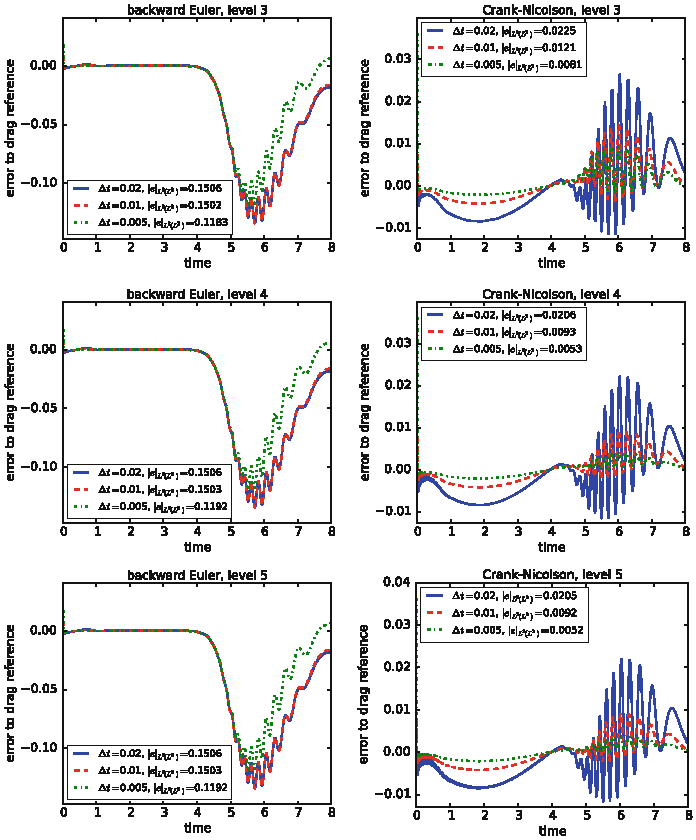
\includegraphics[width=\linewidth]{figures/Chapter_07/Fig_7_03__PDFp411__Bookp401.pdf}
\captionof{figure}{例题\hyperref[ex:time-dependent-accuracy]{7.58}:阻力系数相对于图\hyperref[fig:appendix-d-10]{D.10}中参考曲线的误差;$Q_2/P_1^{\mathrm{disc}}$ 元对,第 3--5 层(自上而下);左:后向 Euler 格式,右:Crank--Nicolson 格式.两侧均比较了不同的时间步长.}
\label{fig:time-dependent-drag-error}
\end{elegantfigure}

图\hyperref[fig:time-dependent-drag-error]{7.3}--\hyperref[fig:time-dependent-pressure-error]{7.8}给出了计算结果.可以看到,在所有时间离散格式中,后向 Euler 格式所得结果的精度明显最低.本例中,时间误差和空间误差都很重要;采用后向 Euler 格式时,时间误差占主导.若要达到二阶时间格式所能达到的相近误差水平,必须显著缩小时间步长.

\begin{elegantfigure}[\linewidth]
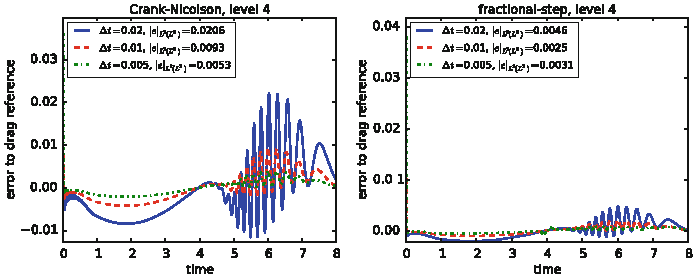
\includegraphics[width=\linewidth]{figures/Chapter_07/Fig_7_04__PDFp412__Bookp402.pdf}
\captionof{figure}{例题\hyperref[ex:time-dependent-accuracy]{7.58}:阻力系数相对于参考曲线的误差;$Q_2/P_1^{\mathrm{disc}}$ 元对;左:Crank--Nicolson 格式,右:分步 $\theta$-格式.}
\label{fig:time-dependent-drag-error-second-order}
\end{elegantfigure}

\begin{elegantfigure}[\linewidth]
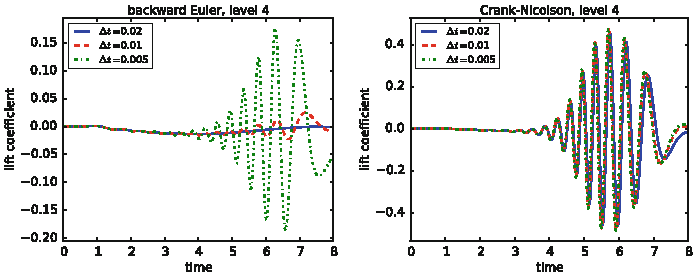
\includegraphics[width=\linewidth]{figures/Chapter_07/Fig_7_05__PDFp412__Bookp402.pdf}
\captionof{figure}{例题\hyperref[ex:time-dependent-accuracy]{7.58}:升力系数随时间的变化;$Q_2/P_1^{\mathrm{disc}}$ 元对;左:后向 Euler 格式,右:Crank--Nicolson 格式.注意两图的尺度不同.}
\label{fig:time-dependent-lift-evolution}
\end{elegantfigure}

升力系数的时间变化(图\hyperref[fig:time-dependent-lift-evolution]{7.5})表明,当时间步长不小于 $\Delta t=0.005$ 时,后向 Euler 格式甚至不能正确预测涡脱落.总的来说,对于空间误差并非占主导的问题,本例展示了高阶空间离散与一阶、二阶时间离散格式结合时,在定性结果上的差异.

\begin{elegantfigure}[\linewidth]
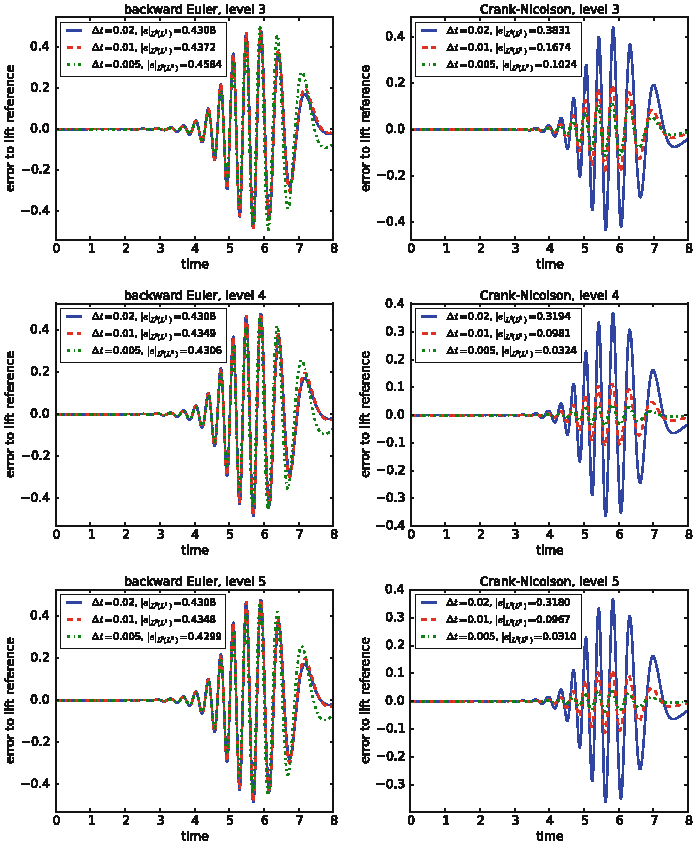
\includegraphics[width=\linewidth]{figures/Chapter_07/Fig_7_06__PDFp413__Bookp403.pdf}
\captionof{figure}{例题\hyperref[ex:time-dependent-accuracy]{7.58}:升力系数相对于图\hyperref[fig:appendix-d-10]{D.10}中参考曲线的误差;$Q_2/P_1^{\mathrm{disc}}$ 元对,第 3--5 层(自上而下);左:后向 Euler 格式,右:Crank--Nicolson 格式.两侧均比较了不同的时间步长.}
\label{fig:time-dependent-lift-error}
\end{elegantfigure}

对于二阶格式,减小时间步长带来的误差下降同样十分明显.二阶时间格式的结果可在图\hyperref[fig:time-dependent-drag-error-second-order]{7.4}、图\hyperref[fig:time-dependent-lift-error-second-order]{7.7}和图\hyperref[fig:time-dependent-pressure-error]{7.8}中比较.尽管 Crank--Nicolson 格式和分步 $\theta$-格式具有相同的阶数,仍可观察到,分步 $\theta$-格式计算得到的各系数精确得多.不过,笔记\hyperref[note:theta-scheme-experience]{7.59}将指出,采用分步 $\theta$-格式模拟流动的计算代价(耗时)通常是 Crank--Nicolson 格式的两到三倍.

\begin{elegantfigure}[\linewidth]
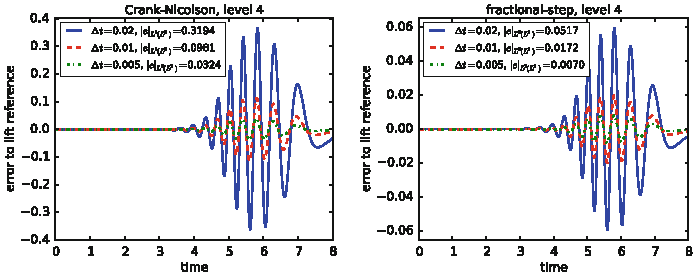
\includegraphics[width=\linewidth]{figures/Chapter_07/Fig_7_07__PDFp414__Bookp404.pdf}
\captionof{figure}{例题\hyperref[ex:time-dependent-accuracy]{7.58}:升力系数相对于图\hyperref[fig:appendix-d-10]{D.10}中参考曲线的误差;$Q_2/P_1^{\mathrm{disc}}$ 元对;左:Crank--Nicolson 格式,右:分步 $\theta$-格式.注意两图的尺度不同.}
\label{fig:time-dependent-lift-error-second-order}
\end{elegantfigure}

\begin{elegantfigure}[\linewidth]
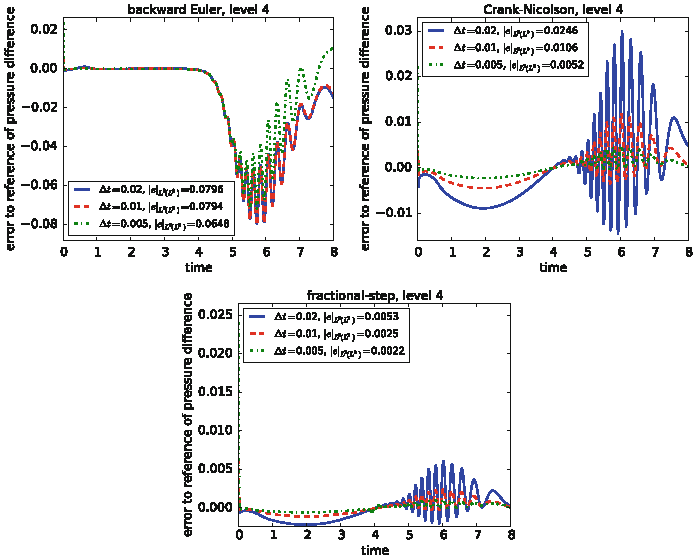
\includegraphics[width=\linewidth]{figures/Chapter_07/Fig_7_08__PDFp414__Bookp404.pdf}
\captionof{figure}{例题\hyperref[ex:time-dependent-accuracy]{7.58}:圆柱前后压差相对于图\hyperref[fig:appendix-d-10]{D.10}中参考曲线的误差;$Q_2/P_1^{\mathrm{disc}}$ 元对;后向 Euler、Crank--Nicolson 和分步 $\theta$-格式的结果按从左到右、从上到下排列.}
\label{fig:time-dependent-pressure-error}
\end{elegantfigure}

在每个离散时刻求解非线性问题时,停止准则的选择颇为微妙.若准则过严,各离散时刻的求解可能耗时很长,从而显著增加总计算时间,但预期可以得到精确结果.相反,采用较宽松的准则可能大幅加快模拟;然而,某些离散时刻的解可能相当不准确,使整体误差明显增大,见图\hyperref[fig:time-dependent-stopping-tolerance]{7.9}.

\begin{elegantfigure}[\linewidth]
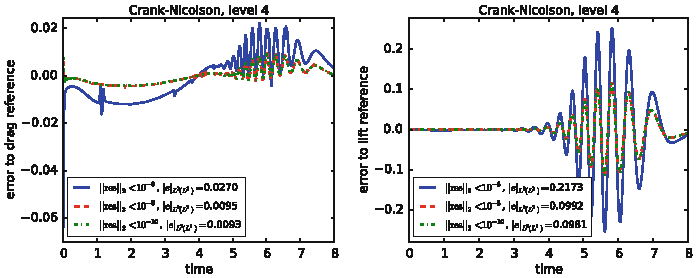
\includegraphics[width=\linewidth]{figures/Chapter_07/Fig_7_09__PDFp415__Bookp405.pdf}
\captionof{figure}{例题\hyperref[ex:time-dependent-accuracy]{7.58}:各离散时刻 Picard 迭代的停止准则对计算精度的影响;$Q_2/P_1^{\mathrm{disc}}$ 元对,Crank--Nicolson 格式,$\Delta t=0.01$.}
\label{fig:time-dependent-stopping-tolerance}
\end{elegantfigure}

图\hyperref[fig:time-dependent-stopping-tolerance]{7.9}显示,与残量向量欧几里得范数不超过 $10^{-6}$ 相比,将其作为停止准则并要求范数不超过 $10^{-8}$,精度会明显提高.据观察,容差取 $10^{-8}$ 时的计算时间约为容差取 $10^{-6}$ 时的 $2.5$ 倍.将容差进一步减小至 $10^{-10}$,相较于 $10^{-8}$ 并不能明显提高精度,但计算时间又增加了约 $2.8$ 倍.何为“严格”或“宽松”的停止准则,取决于具体问题和所用方法.
\index{停止准则}
\end{example}

\begin{note}[Navier--Stokes 方程隐式 $\theta$-格式的数值经验]
\label{note:theta-scheme-experience}
Crank--Nicolson 格式和分步 $\theta$-格式已在 Navier--Stokes 方程中得到充分检验和比较;综述可参见 \textcite{Emmrich2001}.Crank--Nicolson 格式是 A-稳定的,而分步 $\theta$-格式甚至具有强 A-稳定性.这意味着,当初始数据或边界条件不光滑时,Crank--Nicolson 格式可能引起数值振荡;只有采用足够小的时间步,这些振荡才会衰减.与分步 $\theta$-格式相比,为保证 Crank--Nicolson 格式的稳健性,可能需要采用更小的时间步.

二维 Navier--Stokes 方程的数值试验\parencite{JohnRang2010,JohnMatthiesRang2006a}表明,分步 $\theta$-格式所得结果通常比 Crank--Nicolson 格式略精确.不过,分步 $\theta$-格式的计算时间通常是 Crank--Nicolson 格式的两到三倍.总的来说,从单位 CPU 时间所能获得的精度来看,\textcite{JohnRang2010}的结果图中 Crank--Nicolson 格式略占优势.
\index{Crank--Nicolson 格式}
\end{note}

\begin{note}[实现]
\label{note:theta-scheme-implementation}
有限元 $\theta$-格式的基本实现步骤与 Stokes 方程和 Oseen 方程相同,参见第\hyperref[sec:stokes-fem-implementation]{4.3 节}和笔记\hyperref[note:oseen-fem-implementation]{5.19}.表示时间导数离散所需的矩阵只有质量矩阵
\begin{equation}\label{eq:theta-temporal-mass-matrix}
  (M)_{ij}=(\varphi_j^h,\varphi_i^h)_K,\qquad
  i,j=1,\ldots,3N_v.
\end{equation}

对于 Picard 迭代系统\hyperref[eq:general-theta-picard]{(7.85)},若黏性项采用梯度形式,对流项采用对流形式、散度形式或斜对称形式,则代数系统的矩阵为
\[
\resizebox{\linewidth}{!}{$\displaystyle
\begin{pmatrix}
M&0&0&0\\
0&M&0&0\\
0&0&M&0\\
0&0&0&0
\end{pmatrix}
+\Delta t_{n+1}
\begin{pmatrix}
\theta_1A_{11}(\bm{u}_{k+1}^{(m)})&0&0&
\dfrac{\Delta t_{k+1}}{\Delta t_{n+1}}B_1^{\mathsf T}\\
0&\theta_1A_{11}(\bm{u}_{k+1}^{(m)})&0&
\dfrac{\Delta t_{k+1}}{\Delta t_{n+1}}B_2^{\mathsf T}\\
0&0&\theta_1A_{11}(\bm{u}_{k+1}^{(m)})&
\dfrac{\Delta t_{k+1}}{\Delta t_{n+1}}B_3^{\mathsf T}\\
\dfrac{\Delta t_{k+1}}{\Delta t_{n+1}}B_1&
\dfrac{\Delta t_{k+1}}{\Delta t_{n+1}}B_2&
\dfrac{\Delta t_{k+1}}{\Delta t_{n+1}}B_3&0
\end{pmatrix}.
$}
\]
式\hyperref[eq:general-theta-picard]{(7.85)}右端含 $\theta_2$ 的项具有如下矩阵形式:
\begin{equation}\label{eq:picard-explicit-rhs-matrix}
\begin{aligned}
  -\theta_2\Delta t_{n+1}
  \begin{pmatrix}
    A_{11}(\bm{u}_k)&0&0&0\\
    0&A_{11}(\bm{u}_k)&0&0\\
    0&0&A_{11}(\bm{u}_k)&0\\
    0&0&0&0
  \end{pmatrix}
  \begin{pmatrix}\bm{u}_k\\0\end{pmatrix}.
\end{aligned}
\end{equation}
这里,$A_{11}(\bm{u}_k)$ 是在离散时刻 $t_k$ 的 Picard 迭代中最后一次组装得到的矩阵.因此,计算式\hyperref[eq:picard-explicit-rhs-matrix]{(7.88)}只需进行一次矩阵--向量乘法.
\end{note}

\begin{note}[半隐式方法(IMEX 格式)]
\label{note:imex-schemes}\label{note:oseen-semi-implicit}
一种常用方法是采用半隐式格式,即 IMEX(implicit-explicit,隐式--显式)格式.它避免在每个离散时刻求解非线性问题,因此相较于全隐式格式,采用 IMEX 格式进行模拟有望减少计算耗时.

在这类格式中,将一般格式\hyperref[eq:general-theta-scheme]{(7.83)}中出现的非线性项 $(\bm{u}_{k+1}\cdot\nabla)\bm{u}_{k+1}$ 替换为 $(\bm{u}_{\mathrm{prev}}\cdot\nabla)\bm{u}_{k+1}$,其中 $\bm{u}_{\mathrm{prev}}$ 可由已经计算出的解得到.最简单的取法是令 $\bm{u}_{\mathrm{prev}}=\bm{u}_k$,但也常采用前两个时间步的解作线性外推,即
\begin{equation}\label{eq:linear-velocity-extrapolation}
  \bm{u}_{\mathrm{prev}}
  =\frac{\Delta t_{k+1}}{\Delta t_k}
    (\bm{u}_k-\bm{u}_{k-1})+\bm{u}_k.
\end{equation}
\index{IMEX 格式}

当 $\theta=0.5$ 时,这一线性外推(linear extrapolation)所得到的格式与 \textcite{Ingram2013a} 提出并研究的稳定化外推 Crank--Nicolson 格式 CNLE(stab) 类似.对于等时间步长,该文中的对流项为
\begin{equation}\label{eq:cnle-stabilized-convective-term}
\begin{aligned}
  \frac{1}{4}\Delta t\Bigl[
    &(((2\bm{u}_n+\bm{u}_{n-1}-\bm{u}_{n-2})
       \cdot\nabla)\bm{u}_{n+1},\bm{v})\\
    &+(( (2\bm{u}_n+\bm{u}_{n-1}-\bm{u}_{n-2})
       \cdot\nabla)\bm{u}_{n},\bm{v})
  \Bigr].
\end{aligned}
\end{equation}
而采用外推式\hyperref[eq:linear-velocity-extrapolation]{(7.89)}时,所得对流项为
\begin{equation}\label{eq:imex-cnle-convective-term}
\begin{aligned}
  \frac{1}{2}\Delta t\Bigl[
    &(((2\bm{u}_n-\bm{u}_{n-1})
       \cdot\nabla)\bm{u}_{n+1},\bm{v})\\
    &+(( (2\bm{u}_{n-1}-\bm{u}_{n-2})
       \cdot\nabla)\bm{u}_{n},\bm{v})
  \Bigr].
\end{aligned}
\end{equation}
式\hyperref[eq:cnle-stabilized-convective-term]{(7.90)}和式\hyperref[eq:imex-cnle-convective-term]{(7.91)}中的第二项均出现在时间 $t_{n+1}$ 对应方程的右端.注意,
\[
  \frac{2}{4}(2\bm{u}_n+\bm{u}_{n-1}-\bm{u}_{n-2})
  =\frac{1}{2}(2\bm{u}_n-\bm{u}_{n-1})
   +\frac{1}{2}(2\bm{u}_{n-1}-\bm{u}_{n-2}),
\]
因此,式\hyperref[eq:cnle-stabilized-convective-term]{(7.90)}和式\hyperref[eq:imex-cnle-convective-term]{(7.91)}将外推速度场以不同方式分配给离散时刻 $t_{n+1}$ 和 $t_n$ 对应的项.式\hyperref[eq:imex-cnle-convective-term]{(7.91)}使得在 $t_{n+1}$ 时计算方程右端时,可以使用在 $t_n$ 组装的矩阵,参见笔记\hyperref[note:theta-scheme-implementation]{7.60}.
\end{note}

\begin{example}[\enspace IMEX 格式]
\label{ex:imex-schemes-cylinder}
为展示 IMEX 格式的性能,考虑具有定常入口流的二维绕圆柱流动,即例题\hyperref[ex:appendix-d-8]{D.8}.模拟采用 $Q_2/P_1^{\mathrm{disc}}$ 元对;初始网格见图\hyperref[fig:steady-ns-cylinder-initial-grids]{6.5},自由度数见表\hyperref[tab:time-dependent-cylinder-dofs]{7.4}.Crank--Nicolson 格式的时间步长取 $\Delta t=0.005$.IMEX 格式分别采用常值外推 $\bm{u}_{\mathrm{prev}}=\bm{u}_n$ 和线性外推式\hyperref[eq:imex-cnle-convective-term]{(7.91)}.

图\hyperref[fig:imex-cylinder-quantities]{7.10}给出了第 4 层网格上的结果;第 3 层和第 5 层上的结果在定性上相同.可以看到,采用常值外推的 IMEX 格式精度较差,例如阻力系数和升力系数的最大值都明显偏大.\textcite{CaiazzoIliescuJohnSchyschlowa2014}在后向 Euler 格式配合常值外推时也观察到相同现象.相反,IMEX 格式采用线性外推时,结果精度几乎与全隐式格式相同.

\textcite{TabataTagami2000}对后向 Euler 格式配合常值外推时计算得到的阻力系数和升力系数作了数值分析.该分析假定 Navier--Stokes 方程的解具有足够的正则性.然而,重要量为阻力和升力的绕物体流动问题,其计算区域通常不是凸域,因此这一假设是否成立并不明确.

效率提升幅度取决于许多因素,例如具体问题、所用求解器和实现细节.对于本例给出的数值结果,IMEX 格式采用稀疏直接求解器 UMFPACK,参见 \textcite{Davis2004};该求解器用于 IMEX 格式的情况亦见第\hyperref[note:chapter9-solver-choice]{9.5 条笔记}.

\begin{elegantfigure}[\linewidth]
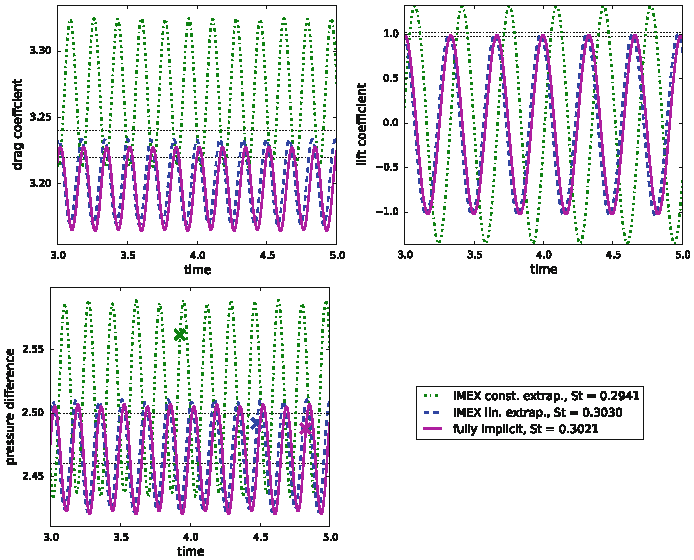
\includegraphics[width=\linewidth]{figures/Chapter_07/Fig_7_10__PDFp418__Bookp408.pdf}
\captionof{figure}{例题\hyperref[ex:imex-schemes-cylinder]{7.62}:感兴趣量.表\hyperref[tab:appendix-d-2]{D.2}中的参考区间以虚线表示;叉号表示周期的中点.Strouhal 数的参考区间为 $[0.295,0.305]$.}
\label{fig:imex-cylinder-quantities}
\end{elegantfigure}

全隐式格式则采用 Picard 迭代,并对线性系统作非精确求解:残量向量的欧几里得范数每次缩小至原来的十分之一,Picard 迭代的停止准则为该范数小于 $10^{-8}$.求解器采用带耦合多重网格预条件子的 FGMRES 方法,见第\hyperref[subsec:chapter9-iterative-solvers]{9.2.2 节}.本例中,IMEX 格式在第 3、4、5 层上的模拟分别快约 $40$ 倍、$10$ 倍和 $2.25$ 倍.网格越细,效率提升幅度越小,因为细化网格时,迭代求解器的扩展性优于稀疏直接求解器.
\end{example}

\begin{note}[自适应时间步长控制]
\label{note:adaptive-time-step-control}
常微分方程数值模拟中的自适应时间步长控制(adaptive time-step control)已有成熟方法,例如参见 \textcite[第 II.4 节]{HairerNoersettWanner1993}.这些方法通过比较由不同阶数的方法得到的两个解,并利用所谓的控制器(controller)确定下一时间步的长度.若条件允许,可采用所谓的嵌入格式(embedded scheme),以较低计算代价求得比原时间离散格式低一阶的近似解.然而,$\theta$-格式这一类方法没有嵌入格式,因此需要采用其他自适应时间步长控制方法.
\index{自适应时间步长控制}

\textcite{Turek1999}提出通过比较分步 $\theta$-格式和 Crank--Nicolson 格式的结果来控制时间步长.这两种格式的误差展开式首项具有不同的常数;利用该差异和两种格式所得解之间的差异,可以预测合适的时间步长.这种方法的主要缺点是计算代价高:Crank--Nicolson 格式这一步只用于确定下一时间步的长度,而其计算成本不可忽略,因此会显著增加每个时间步的开销.\textcite{KayGreshoGriffithsSilvester2010}提出了类似但代价较低的方法,即比较 Crank--Nicolson 格式与二阶显式 Adams--Bashforth 方法所得的速度解来控制步长.另一种更具启发性的做法,是在某个范数下监测已计算解的变化,并据此调整时间步长,例如参见 \textcite{BerroneMarro2009}.
\end{note}
\subsection{其他格式}\label{subsec:time-dependent-other-schemes}

\begin{note}[二阶后向差分公式(BDF2)]
\label{note:bdf2-scheme}
将二阶后向差分公式(backward differentiation formula of order two,BDF2)用于 Navier--Stokes 方程组\cref{eq:time-dependent-ns-strong},得到
\begin{equation}\label{eq:bdf2-time-discretization}
\begin{aligned}
  &\frac32\bm{u}_{n+1}
   +\Delta t_{n+1}\Bigl[-\nu\Delta\bm{u}_{n+1}
       +(\bm{u}_{n+1}\cdot\nabla)\bm{u}_{n+1}\Bigr]
   +\Delta t_{n+1}\nabla p_{n+1}\\
  &=2\bm{u}_n-\frac12\bm{u}_{n-1}
    -\Delta t_{n+1}\Bigl[-\nu\Delta\bm{u}_n
       +(\bm{u}_n\cdot\nabla)\bm{u}_n\Bigr]
    +\Delta t_{n+1}\bm{f}_{n+1},\\
  0&=\Delta t_{n+1}\nabla\cdot\bm{u}_{n+1},
\end{aligned}
\end{equation}
其中 $n\ge2$.BDF2 是二阶格式,并且具有强 A-稳定性.因此,与 Crank--Nicolson 格式\hyperref[ex:time-dependent-crank-nicolson]{(见例题 7.49)}相比,它阶数相同、稳定性更强,但需要保存 $\bm{u}_{n-1}$.由于阶数较高且稳定,BDF2 是一种常用格式;例如,它是软件包 deal.II 中的标准时间离散格式,见\textcite{BangerthHartmannKanschat2007}.
\index{BDF2}
\end{note}

\begin{note}[高阶方法]
\label{note:time-dependent-higher-order-schemes}
\textcite{JohnMatthiesRang2006a} 比较了三阶、分别具有 $s=3$ 或 $s=4$ 个阶段的 Rosenbrock 方法与 $\theta$-格式.这些方法是线性隐式 Runge--Kutta 格式.每个离散时刻都要用同一个系统矩阵求解 $s$ 个线性鞍点问题.Rosenbrock 方法可以利用嵌入格式有效地控制时间步长.对于\textcite{JohnMatthiesRang2006a} 所研究的二维问题,Rosenbrock 方法所得数值解通常比 $\theta$-格式精确得多;但采用 $\theta$-格式的模拟明显更高效.\textcite{JohnRang2010} 还在二维绕圆柱流动问题(见例题\hyperref[ex:appendix-d-9]{D.9})上研究并比较了最高四阶的 Rosenbrock 方法、对角隐式 Runge--Kutta 方法(diagonally implicit Runge--Kutta,DIRK)与 $\theta$-格式.所有高阶格式,即阶数至少为三的格式,都可以通过嵌入方法自适应地控制时间步长.若采用时间步长控制,则许多高阶方法在精度与 CPU 时间之比方面明显优于 $\theta$-格式.

尽管如此,目前高阶时间推进格式似乎还不常用.
\index{Rosenbrock 方法}
\index{Runge--Kutta 方法!对角隐式}
\end{note}

\section{有限元误差分析:完全离散情形}\label{sec:time-dependent-fem-fully-discrete}

\begin{note}[与时间连续情形的比较及本节内容]
\label{note:fully-discrete-error-analysis-content}
完全离散 Navier--Stokes 方程组的数值分析与第\hyperref[sec:time-dependent-fem-continuous]{7.2 节}介绍的时间连续情形相似.不过,对时间导数作离散会引入一致性误差,其估计将在引理\hyperref[lem:temporal-derivative-consistency]{7.67}中给出.在完全离散情形中,公式里会出现对离散时刻求和,而不再是时空范数.因此,与时间连续情形相比,论述不那么紧凑,处理也略为繁琐.

本节以时间上采用后向 Euler 格式、空间上采用 Galerkin 有限元方法为例,介绍完全离散情形的分析.为简洁起见,误差分析仅给出速度的估计.
\end{note}

\begin{lemma}[时间导数离散的一致性误差]
\label{lem:temporal-derivative-consistency}
设 $v,\partial_t v,\partial_{tt}v\in L^2(t_n,t_{n+1};L^2(\Omega))$,则
\begin{equation}\label{eq:backward-difference-consistency}
  \left\|\partial_t v_{n+1}
      -\frac{v_{n+1}-v_n}{\Delta t}\right\|_{L^2(\Omega)}^2
   \le \Delta t\,\|\partial_{tt}v\|_{L^2(t_n,t_{n+1};L^2(\Omega))}^2.
\end{equation}
若进一步有 $\partial_{ttt}v\in L^2(t_n,t_{n+1};L^2(\Omega))$,则
\begin{equation}\label{eq:midpoint-difference-consistency}
  \left\|\partial_t v_{n+1/2}
      -\frac{v_{n+1}-v_n}{\Delta t}\right\|_{L^2(\Omega)}^2
   \le \Delta t^3\,\|\partial_{ttt}v\|_{L^2(t_n,t_{n+1};L^2(\Omega))}^2.
\end{equation}
\end{lemma}

\begin{proof}
对带积分余项的 Taylor 公式作分部积分,也可得到
\[
  v_n=v_{n+1}-\Delta t\,\partial_t v_{n+1}
       +\int_{t_n}^{t_{n+1}}(t-t_n)\,\partial_{tt}v\,\mathrm{d}t,
\]
这等价于
\[
  \partial_t v_{n+1}-\frac{v_{n+1}-v_n}{\Delta t}
    =\frac1{\Delta t}\int_{t_n}^{t_{n+1}}
       (t-t_n)\,\partial_{tt}v\,\mathrm{d}t.
\]
利用 Cauchy--Schwarz 不等式\hyperref[eq:appendix-a-10]{(A.10)},注意到其中一个因子与空间变量无关,并应用 Fubini 定理,可得
\[
\begin{aligned}
 &\left\|\partial_t v_{n+1}
       -\frac{v_{n+1}-v_n}{\Delta t}\right\|_{L^2(\Omega)}^2\\
 &\quad\le \frac1{\Delta t^2}
   \left(\int_{t_n}^{t_{n+1}}(t-t_n)^2\,\mathrm{d}t\right)
   \left(\int_{t_n}^{t_{n+1}}\int_\Omega
       (\partial_{tt}v)^2\,\mathrm{d}x\,\mathrm{d}t\right)\\
 &\quad=\frac{\Delta t}{3}
       \|\partial_{tt}v\|_{L^2(t_n,t_{n+1};L^2(\Omega))}^2
   \le \Delta t\,\|\partial_{tt}v\|_{L^2(t_n,t_{n+1};L^2(\Omega))}^2,
\end{aligned}
\]
故得\cref{eq:backward-difference-consistency}.这里为简洁起见,将因子 $1/3$ 以 $1$ 代替.

\cref{eq:midpoint-difference-consistency} 的证明方法相同.对任意 $\theta\in[0,1]$ 作 Taylor 展开,或连续分部积分,可得
\[
\begin{aligned}
 v_n={}&v_{n+\theta}-\theta\Delta t\,\partial_t v_{n+\theta}
       +\frac{\theta^2}{2}\Delta t^2\partial_{tt}v_{n+\theta}\\
      &\quad+\frac12\int_{t_n}^{t_{n+\theta}}
          (t_n-t)^2\partial_{ttt}v\,\mathrm{d}t,\\
 v_{n+1}={}&v_{n+\theta}+(1-\theta)\Delta t\,\partial_t v_{n+\theta}
       +\frac{(1-\theta)^2}{2}\Delta t^2\partial_{tt}v_{n+\theta}\\
      &\quad+\frac12\int_{t_{n+\theta}}^{t_{n+1}}
          (t_{n+1}-t)^2\partial_{ttt}v\,\mathrm{d}t.
\end{aligned}
\]
将第二式从第一式中相减并整理,得到
\[
\begin{aligned}
 \partial_t v_{n+\theta}
   ={}&\frac{v_{n+1}-v_n}{\Delta t}
      +\frac{\Delta t}{2}\bigl(\theta^2-(1-\theta)^2\bigr)
          \partial_{tt}v_{n+\theta}\\
     &-\frac1{2\Delta t}\int_{t_n}^{t_{n+\theta}}
          (t_n-t)^2\partial_{ttt}v\,\mathrm{d}t
      \\[-1mm]
     &-\frac1{2\Delta t}\int_{t_{n+\theta}}^{t_{n+1}}
          (t_{n+1}-t)^2\partial_{ttt}v\,\mathrm{d}t.
\end{aligned}
\]
含 $\partial_{tt}v_{n+\theta}$ 的项仅当 $\theta=1/2$ 时才消失.取 $\theta=1/2$,并像证明\cref{eq:backward-difference-consistency} 那样处理,可得
\[
\begin{aligned}
 &\left\|\partial_t v_{n+1/2}
       -\frac{v_{n+1}-v_n}{\Delta t}\right\|_{L^2(\Omega)}^2\\
 &\quad\le\frac1{4\Delta t^2}\Biggl[
   \left(\int_{t_n}^{t_{n+1/2}}(t_n-t)^4\,\mathrm{d}t\right)
   \left(\int_\Omega\int_{t_n}^{t_{n+1/2}}
       (\partial_{ttt}v)^2\,\mathrm{d}t\,\mathrm{d}x\right)\\
 &\qquad\qquad+
   \left(\int_{t_{n+1/2}}^{t_{n+1}}(t_{n+1}-t)^4\,\mathrm{d}t\right)
   \left(\int_\Omega\int_{t_{n+1/2}}^{t_{n+1}}
       (\partial_{ttt}v)^2\,\mathrm{d}t\,\mathrm{d}x\right)
   \Biggr],
\end{aligned}
\]
直接计算即得\cref{eq:midpoint-difference-consistency}.
\end{proof}

\begin{note}[后向 Euler 格式]
\label{note:backward-euler-scheme}
等步长的后向 Euler 格式如下:给定 $\bm{f}_{n+1}\in V'$ 和 $\bm{u}_n^h\in V^h$,通过求解下列问题计算 $(\bm{u}_{n+1}^h,p_{n+1}^h)\in V^h\times Q^h$,其中 $n=0,1,2,\ldots$:
\begin{equation}\label{eq:fully-discrete-backward-euler}
\begin{aligned}
 &\frac1{\Delta t}(\bm{u}_{n+1}^h-\bm{u}_n^h,\bm{v}^h)
   +\nu(\nabla\bm{u}_{n+1}^h,\nabla\bm{v}^h)
   +n_{\mathrm{skew}}(\bm{u}_{n+1}^h,\bm{u}_{n+1}^h,\bm{v}^h)\\
 &\quad-(\nabla\cdot\bm{v}^h,p_{n+1}^h)
       +(\nabla\cdot\bm{u}_{n+1}^h,q^h)
    =\langle\bm{f}_{n+1},\bm{v}^h\rangle_{V',V},\\
 &\hspace{7em}\forall(\bm{v}^h,q^h)\in V^h\times Q^h.
\end{aligned}
\end{equation}
初始条件 $\bm{u}_0^h$ 是将 $\bm{u}_0$ 插值或投影到有限元空间所得的函数,例如 Lagrange 插值或 Stokes 投影\hyperref[eq:stokes-projection-definition]{(4.54)}.
\index{后向 Euler 格式}
\end{note}

\begin{lemma}[有限元解的存在性、唯一性与稳定性]
\label{lem:fully-discrete-backward-euler-existence-stability}
设有限元空间对 $V^h$ 与 $Q^h$ 满足离散 inf-sup 条件\hyperref[eq:discrete-infsup-condition]{(3.51)}.当时间步长足够小时,问题\cref{eq:fully-discrete-backward-euler} 有唯一解.时间步长的限制依赖于网格宽度.

对问题\cref{eq:fully-discrete-backward-euler} 的任意解以及所有 $N\ge0$,均有
\begin{equation}\label{eq:fully-discrete-backward-euler-stability}
  \begin{aligned}
    &\|\bm{u}_{N+1}^h\|_{L^2(\Omega)}^2\\
    &+\nu\Delta t\sum_{n=0}^{N}
         \|\nabla\bm{u}_{n+1}^h\|_{L^2(\Omega)}^2\\
    &\le \|\bm{u}_0^h\|_{L^2(\Omega)}^2\\
    &\quad+\frac{\Delta t}{\nu}\sum_{n=0}^{N}
         \|\bm{f}_{n+1}\|_{H^{-1}(\Omega)}^2.
  \end{aligned}
\end{equation}
\end{lemma}

\begin{proof}
先证明稳定性估计\cref{eq:fully-discrete-backward-euler-stability},因为随后证明解的存在性和唯一性时会用到该估计.

\textit{稳定性.} 按通常方法,在问题\cref{eq:fully-discrete-backward-euler} 中取任意解作为检验函数,即令 $(\bm{v}^h,q^h)=(\bm{u}_{n+1}^h,p_{n+1}^h)$.由对流项的斜对称性\hyperref[eq:steady-ns-nskew-definition]{(6.25)},有
$n_{\mathrm{skew}}(\bm{u}_{n+1}^h,\bm{u}_{n+1}^h,\bm{u}_{n+1}^h)=0$,因而
\begin{equation}\label{eq:fully-discrete-backward-euler-energy}
  \frac1{\Delta t}(\bm{u}_{n+1}^h-\bm{u}_n^h,\bm{u}_{n+1}^h)
   +\nu\|\nabla\bm{u}_{n+1}^h\|_{L^2(\Omega)}^2
    =\langle\bm{f}_{n+1},\bm{u}_{n+1}^h\rangle_{V',V}.
\end{equation}
类似于实数 $a,b$ 的代数关系
$a^2-ab=\tfrac12\bigl(a^2+(a-b)^2-b^2\bigr)$,有
\begin{equation}\label{eq:backward-euler-time-difference-identity}
\begin{aligned}
 (\bm{u}_{n+1}^h-\bm{u}_n^h,\bm{u}_{n+1}^h)
  =\frac12\Bigl(&\|\bm{u}_{n+1}^h\|_{L^2(\Omega)}^2
       +\|\bm{u}_{n+1}^h-\bm{u}_n^h\|_{L^2(\Omega)}^2\\
       &-\|\bm{u}_n^h\|_{L^2(\Omega)}^2\Bigr).
\end{aligned}
\end{equation}
将\cref{eq:backward-euler-time-difference-identity}代入\cref{eq:fully-discrete-backward-euler-energy},并利用
$\|\bm{u}_{n+1}^h-\bm{u}_n^h\|_{L^2(\Omega)}^2\ge0$,可得
\[
  \|\bm{u}_{n+1}^h\|_{L^2(\Omega)}^2
   +2\nu\Delta t\|\nabla\bm{u}_{n+1}^h\|_{L^2(\Omega)}^2
  \le \|\bm{u}_n^h\|_{L^2(\Omega)}^2
     +2\Delta t\langle\bm{f}_{n+1},\bm{u}_{n+1}^h\rangle_{V',V}.
\]
对偶配对估计和 Young 不等式\hyperref[eq:appendix-a-5]{(A.5)}给出
\[
  \|\bm{u}_{n+1}^h\|_{L^2(\Omega)}^2
   +\nu\Delta t\|\nabla\bm{u}_{n+1}^h\|_{L^2(\Omega)}^2
  \le \|\bm{u}_n^h\|_{L^2(\Omega)}^2
     +\frac{\Delta t}{\nu}
       \|\bm{f}_{n+1}\|_{H^{-1}(\Omega)}^2.
\]
从 $n=0$ 到 $N$ 求和,并注意两边的第一项形成望远镜求和,即得稳定性估计\cref{eq:fully-discrete-backward-euler-stability}.

\textit{解的存在性与唯一性.} 后向 Euler 格式\cref{eq:fully-discrete-backward-euler} 在每个离散时刻都要求解一个非线性离散问题,其形式与定常 Navier--Stokes 方程组相似,只是多了由时间离散产生的项.解的存在性与唯一性可用与定常 Navier--Stokes 方程组相同的方法证明,参见定理\hyperref[thm:steady-ns-existence]{6.17}的证明.考虑 Oseen 型问题:给定 $\bm{f}_{n+1}\in V'$ 以及 $\bm{b}^h,\bm{u}_n^h\in V_{\mathrm{div}}^h$,求 $\bm{u}^h\in V_{\mathrm{div}}^h$,使得
\begin{equation}\label{eq:fully-discrete-backward-euler-oseen}
  \begin{aligned}
   &\frac1{\Delta t}(\bm{u}^h,\bm{v}^h)
      +\nu(\nabla\bm{u}^h,\nabla\bm{v}^h)
      +n_{\mathrm{skew}}(\bm{b}^h,\bm{u}^h,\bm{v}^h)\\
   &\quad=\frac1{\Delta t}(\bm{u}_n^h,\bm{v}^h)
      +\langle\bm{f}_{n+1},\bm{v}^h\rangle_{V',V},\\
   &\hspace{8em}\forall\bm{v}^h\in V_{\mathrm{div}}^h.
  \end{aligned}
\end{equation}
由此定义算子
\[
  \mathcal N_{\mathrm{conv}}^h:V_{\mathrm{div}}^h\to V_{\mathrm{div}}^h,
  \qquad \bm{b}^h\mapsto\bm{u}^h.
\]
问题\cref{eq:fully-discrete-backward-euler-oseen} 对每个给定的 $\bm{b}^h$ 都有唯一解;这一点由 Lax--Milgram 定理得到,细节参见引理\hyperref[lem:imex-euler-existence-uniqueness-stability]{7.77}的证明.算子 $\mathcal N_{\mathrm{conv}}^h$ 的每个不动点都是后向 Euler 问题\cref{eq:fully-discrete-backward-euler} 在时刻 $t_{n+1}$ 的一个速度解.由于当检验函数为 $\bm{v}^h=\bm{u}^h$ 时,对流项消失,仿照稳定性估计的第一部分可得
\begin{equation}\label{eq:fully-discrete-backward-euler-oseen-stability}
  \|\bm{u}^h\|_{L^2(\Omega)}^2
   +\nu\Delta t\|\nabla\bm{u}^h\|_{L^2(\Omega)}^2
  \le \|\bm{u}_n^h\|_{L^2(\Omega)}^2
     +\frac{\Delta t}{\nu}\|\bm{f}_{n+1}\|_{H^{-1}(\Omega)}^2.
\end{equation}
由此可见,算子 $\mathcal N_{\mathrm{conv}}^h$ 关于 $\bm{b}^h$ 有界,且界与 $\bm{b}^h$ 无关:
\[
\begin{aligned}
 \|\mathcal N_{\mathrm{conv}}^h\|
  &=\sup_{\substack{\bm{b}^h\in V_{\mathrm{div}}^h\\
                     \|\bm{b}^h\|_V=1}}
       \|\mathcal N_{\mathrm{conv}}^h\bm{b}^h\|_V
   =\sup_{\substack{\bm{b}^h\in V_{\mathrm{div}}^h\\
                     \|\bm{b}^h\|_V=1}}\|\bm{u}^h\|_V\\
  &\le\left(\frac1{\nu\Delta t}\|\bm{u}_n^h\|_{L^2(\Omega)}^2
       +\frac1{\nu^2}\|\bm{f}_{n+1}\|_{H^{-1}(\Omega)}^2\right)^{1/2}.
\end{aligned}
\]
在估计\cref{eq:fully-discrete-backward-euler-oseen-stability}左端的第一项中应用逆估计\hyperref[eq:appendix-c-37]{(C.37)},得到
\begin{equation}\label{eq:fully-discrete-backward-euler-inverse-bound}
  \|\nabla\bm{u}^h\|_{L^2(\Omega)}^2
   \le\frac1{C_{\mathrm{inv}}^{-2}h^2+\nu\Delta t}
       \left(\|\bm{u}_n^h\|_{L^2(\Omega)}^2
         +\frac{\Delta t}{\nu}
             \|\bm{f}_{n+1}\|_{H^{-1}(\Omega)}^2\right).
\end{equation}
任取 $\bm{b}_1^h,\bm{b}_2^h\in V_{\mathrm{div}}^h$,令
$\bm{u}_1^h=\mathcal N_{\mathrm{conv}}^h\bm{b}_1^h$、
$\bm{u}_2^h=\mathcal N_{\mathrm{conv}}^h\bm{b}_2^h$,并将相应问题相减.取
$\bm{v}^h=\bm{u}_1^h-\bm{u}_2^h$,可得
\begin{equation}\label{eq:fully-discrete-backward-euler-operator-difference}
\begin{aligned}
 &\frac1{\Delta t}\|\bm{u}_1^h-\bm{u}_2^h\|_{L^2(\Omega)}^2
   +\nu\|\nabla(\bm{u}_1^h-\bm{u}_2^h)\|_{L^2(\Omega)}^2\\
 &\qquad=-n_{\mathrm{skew}}(\bm{b}_1^h-\bm{b}_2^h,
              \bm{u}_1^h,\bm{u}_1^h-\bm{u}_2^h).
\end{aligned}
\end{equation}
对\cref{eq:fully-discrete-backward-euler-operator-difference}左端第一项应用逆估计,并利用对流项估计\hyperref[eq:steady-ns-conv-estimate-29]{(6.29)},得到
\[
\begin{aligned}
 &\left(\frac{C_{\mathrm{inv}}^{-2}h^2}{\Delta t}+\nu\right)
      \|\nabla(\bm{u}_1^h-\bm{u}_2^h)\|_{L^2(\Omega)}^2\\
 &\quad\le N_{\mathrm{div}}^h\|\bm{b}_1^h-\bm{b}_2^h\|_V
      \|\bm{u}_1^h\|_V\\
 &\hspace{8em}\times\|\nabla(\bm{u}_1^h-\bm{u}_2^h)\|_{L^2(\Omega)},
\end{aligned}
\]
其中 $N_{\mathrm{div}}^h$ 由\hyperref[eq:steady-ns-discrete-convection-norm]{(6.57)}定义.再代入\cref{eq:fully-discrete-backward-euler-inverse-bound},可得
\[
\begin{aligned}
 &\|\nabla(\bm{u}_1^h-\bm{u}_2^h)\|_{L^2(\Omega)}\\
 &\quad\le N_{\mathrm{div}}^h\Delta t
       \left(\frac1{C_{\mathrm{inv}}^{-2}h^2+\nu\Delta t}\right)^{3/2}\\
 &\qquad\times\left(\|\bm{u}_n^h\|_{L^2(\Omega)}^2
          +\frac{\Delta t}{\nu}
              \|\bm{f}_{n+1}\|_{H^{-1}(\Omega)}^2\right)^{1/2}\\
 &\qquad\times\|\bm{b}_1^h-\bm{b}_2^h\|_V.
\end{aligned}
\]
当时间步长足够小时,$\|\bm{b}_1^h-\bm{b}_2^h\|_V$ 前的系数小于 $1$.此时由 Banach 不动点定理\hyperref[thm:appendix-a-68]{A.68},问题\cref{eq:fully-discrete-backward-euler} 的速度解存在且唯一.时刻 $t_{n+1}$ 的压力解存在且唯一,则由有限元空间满足离散 inf-sup 条件可知.
\end{proof}

\begin{note}[关于解的存在性与唯一性]
\label{note:fully-discrete-solution-existence-uniqueness}
问题\cref{eq:fully-discrete-backward-euler} 与定常 Navier--Stokes 方程组形式相近.对任意长度的时间步证明解的存在性,可采用与定常 Navier--Stokes 方程组存在性证明相同的方法,参见\textcite[第 15.2 节]{MarionTemam1998}以及定理\hyperref[thm:steady-ns-existence]{6.17}证明中所引的文献.

若对解作更强的正则性假设,则可以证明:当时间步长足够小时,解唯一,且时间步长条件不依赖网格尺寸.例如,假设 $\nabla\bm{u}\in L^\infty(0,T;L^2(\Omega))$,\textcite[式(3.15)]{HeywoodRannacher1990}证明了
$\|\nabla\bm{u}^h\|_{L^\infty(0,T;L^2(\Omega))}<C$,其中常数 $C$ 与 $h$ 无关.将此界代入\cref{eq:fully-discrete-backward-euler-inverse-bound},便得到一个不依赖网格宽度的时间步长条件.

另一种做法是先证明解存在,再在时间步长足够小时证明唯一性.假设有两个解 $\bm{u}_1^h$ 和 $\bm{u}_2^h$,将它们的方程相减,并以两解之差作为检验函数,得到
\begin{equation}\label{eq:fully-discrete-backward-euler-uniqueness}
\begin{aligned}
 &\frac1{\Delta t}\|\bm{u}_1^h-\bm{u}_2^h\|_{L^2(\Omega)}^2
    +\nu\|\nabla(\bm{u}_1^h-\bm{u}_2^h)\|_{L^2(\Omega)}^2\\
 &=-n_{\mathrm{skew}}(\bm{u}_1^h,\bm{u}_1^h,
                   \bm{u}_1^h-\bm{u}_2^h)
    +n_{\mathrm{skew}}(\bm{u}_2^h,\bm{u}_1^h,
                   \bm{u}_1^h-\bm{u}_2^h)\\
 &=n_{\mathrm{conv}}(\bm{u}_1^h-\bm{u}_2^h,\bm{u}_1^h,
                    \bm{u}_1^h-\bm{u}_2^h)\\
 &\quad+\frac12\bigl(\nabla\cdot(\bm{u}_1^h-\bm{u}_2^h),
                \bm{u}_1^h\cdot(\bm{u}_1^h-\bm{u}_2^h)\bigr).
\end{aligned}
\end{equation}
这里用到了斜对称型的定义\hyperref[eq:steady-ns-nskew-definition]{(6.25)}和\hyperref[eq:steady-ns-conv-form-4]{(6.13)}.若假设 $\bm{u}_1^h\in L^\infty((0,T);L^\infty(\Omega))$,则\cref{eq:fully-discrete-backward-euler-uniqueness}右端可估计为
\[
  \frac32\|\bm{u}_1^h\|_{L^\infty(\Omega)}
       \|\bm{u}_1^h-\bm{u}_2^h\|_{L^2(\Omega)}
       \|\nabla(\bm{u}_1^h-\bm{u}_2^h)\|_{L^2(\Omega)}.
\]
在此假设下,$\|\bm{u}_1^h\|_{L^\infty(\Omega)}$ 可由一个与 $h$ 无关的常数控制,见\textcite[式(2.16)及注记 5.1]{deFrutos2008}.随后应用 Young 不等式\hyperref[eq:appendix-a-5]{(A.5)},可得只有在时间步长足够小时才能成立的不等式;这一时间步长限制不依赖 $h$.
\end{note}

\begin{note}[时空范数的近似]
\label{note:time-space-norm-approximation}
设 $X$ 是赋范空间,范数为 $\|\cdot\|_X$.对 $p\in[1,\infty)$、$0\le t_0<t_N$ 以及 $v\in L^p(t_0,t_N;X)$,函数 $v$ 的范数的 $p$ 次幂为
\begin{equation}\label{eq:time-space-norm-integral}
  \|v\|_{L^p(t_0,t_N;X)}^p
    =\int_{t_0}^{t_N}\|v\|_X^p\,\mathrm{d}t.
\end{equation}
式\cref{eq:time-space-norm-integral}可用复合梯形公式(composite trapezoidal rule)近似.为此,将区间 $[t_0,t_N]$ 划分为长度均为 $\Delta t$ 的子区间.在每个子区间上应用梯形公式
\[
  \int_{t_n}^{t_{n+1}}\|v\|_X^p\,\mathrm{d}t
    \approx\frac{\Delta t}{2}
       \Bigl(\|v(t_{n+1})\|_X^p+\|v(t_n)\|_X^p\Bigr).
\]
将所有子区间上的近似值相加,便得到\cref{eq:time-space-norm-integral}的如下近似:
\[
  \|v\|_{L^p(t_0,t_N;X)}^p
    \approx\Delta t\left(
       \frac{\|v(t_0)\|_X^p}{2}
       +\sum_{n=1}^{N-1}\|v(t_n)\|_X^p
       +\frac{\|v(t_N)\|_X^p}{2}\right).
\]
由此可见,估计\cref{eq:fully-discrete-backward-euler-stability}中的求和项就是复合梯形公式的近似.例如,
\[
  \|\nabla\bm{u}^h\|_{L^2(t_1,t_{N+1};L^2(\Omega))}^2
    \approx\Delta t\sum_{n=0}^{N}
       \|\nabla\bm{u}_{n+1}^h\|_{L^2(\Omega)}^2.
\]
\index{复合梯形公式}
\end{note}

\begin{theorem}[后向 Euler 格式与 Galerkin 有限元方法的速度误差估计]
\label{thm:fully-discrete-backward-euler-velocity-error}\label{thm:time-dependent-fem-fully-discrete-error}
设 $\Omega\subset\mathbb R^d$ 为有界多面体域,$d\in\{2,3\}$,且其边界为 Lipschitz 连续边界.设
$\bm{f}\in L^2(0,T;V')$、$\bm{u}_0\in H_{\mathrm{div}}(\Omega)$、
$\bm{u}_0^h\in V_{\mathrm{div}}^h$,并假设 Navier--Stokes 方程组\cref{eq:time-dependent-ns-weak-first} 的解 $(\bm{u},p)$ 满足
\begin{equation}\label{eq:fully-discrete-backward-euler-error-regularity}
\begin{aligned}
  \partial_{tt}\bm{u}&\in L^2(0,T;H^1(\Omega)),
  &\partial_t\bm{u}&\in L^2(0,T;V'),\\
  \nabla\bm{u}&\in L^4(0,T;L^2(\Omega)),
  &p&\in L^2(0,T;L^2(\Omega)).
\end{aligned}
\end{equation}
以下记 $\bm{u}_n=\bm{u}(t_n)$、$p_n=p(t_n)$.考虑时间上采用后向 Euler 格式、空间上采用 Galerkin 有限元方法的离散\cref{eq:fully-discrete-backward-euler}.设空间对 $V^h\times Q^h$ 满足 inf-sup 条件,时间步长均匀为 $\Delta t$,即 $t_n=n\Delta t$.假设引理\hyperref[lem:fully-discrete-backward-euler-existence-stability]{7.69}中的条件成立,并且时间步长足够小,使得
\begin{equation}\label{eq:fully-discrete-backward-euler-timestep-condition}
  \alpha_n\Delta t
   =C\frac{\|\nabla\bm{u}_n\|_{L^2(\Omega)}^4}{\nu^3}\Delta t<1,
   \qquad n=1,\ldots,N+1.
\end{equation}
则对所有 $N\ge0$,有如下误差估计:
\begin{equation}\label{eq:fully-discrete-backward-euler-velocity-error}
\begin{aligned}
 &\|\bm{u}_{N+1}-\bm{u}_{N+1}^h\|_{L^2(\Omega)}^2
   +\nu\Delta t\sum_{n=1}^{N+1}
       \|\nabla(\bm{u}_n-\bm{u}_n^h)\|_{L^2(\Omega)}^2\\
 &\le C\Biggl\{
       \|\bm{u}_{N+1}-I_h^{\mathrm{St}}\bm{u}_{N+1}\|_{L^2(\Omega)}^2
       +\nu\Delta t\sum_{n=1}^{N+1}
          \|\nabla(\bm{u}_n-I_h^{\mathrm{St}}\bm{u}_n)\|_{L^2(\Omega)}^2\\
 &\quad+\exp\!\left(\Delta t\sum_{n=1}^{N+1}
              \frac{\alpha_n}{1-\Delta t\alpha_n}\right)
       \Biggl[\|\bm{u}_0^h-I_h^{\mathrm{St}}\bm{u}(0)\|_{L^2(\Omega)}^2\\
 &\qquad+\frac{(\Delta t)^2}{\nu}
       \|I_h^{\mathrm{St}}(\partial_{tt}\bm{u})\|_{L^2(0,t_{N+1};L^2(\Omega))}^2\\
  &\qquad+\Delta t\sum_{n=1}^{N+1}\Biggl(
        \frac1\nu\|\partial_t(\bm{u}_n-I_h^{\mathrm{St}}\bm{u}_n)\|_{V'}^2\\
  &\quad+\|\bm{u}_n-I_h^{\mathrm{St}}\bm{u}_n\|_{L^2(\Omega)}
         \|\nabla(\bm{u}_n-I_h^{\mathrm{St}}\bm{u}_n)\|_{L^2(\Omega)}
         \|\nabla\bm{u}_n\|_{L^2(\Omega)}^2\Biggr)\\
 &\qquad+\inf_{q^h\in Q^h}\frac{\Delta t}{\nu}
       \sum_{n=1}^{N+1}\|p_n-q^h\|_{L^2(\Omega)}^2\\
 &\qquad+\frac1{\nu^{3/2}}
       \left(\|\bm{u}_0^h\|_{L^2(\Omega)}^2
          +\frac{\Delta t}{\nu}\sum_{n=0}^{N}
             \|\bm{f}_{n+1}\|_{H^{-1}(\Omega)}^2\right)\\
  &\qquad\times
       \left(\Delta t\sum_{n=1}^{N+1}
          \|\nabla(\bm{u}_n-I_h^{\mathrm{St}}\bm{u}_n)\|_{L^2(\Omega)}^4
       \right)^{1/2}\Biggr]\Biggr\}.
\end{aligned}
\end{equation}
其中 $\alpha_n$ 由\cref{eq:fully-discrete-backward-euler-timestep-condition}定义,$I_h^{\mathrm{St}}\bm{u}_n$ 是 $\bm{u}_n$ 在 $p=0$ 时的 Stokes 投影,见\cref{eq:stokes-projection-definition};并假设
$\partial_t I_h^{\mathrm{St}}\bm{u}\in L^2(0,T;V')$.
\end{theorem}

\begin{proof}
证明主要沿用定理\hyperref[thm:time-dependent-fem-velocity-error]{7.35}的步骤:
\begin{enumerate}
  \item 推导误差方程并分解误差;
  \item 估计误差方程右端的所有项;
  \item 应用离散 Gronwall 引理;
  \item 应用三角不等式.
\end{enumerate}

\textit{1. 推导误差方程并分解误差.} 在时刻 $t_{n+1}$,将误差分解为逼近误差与有限元余项.分解使用\cref{eq:stokes-projection-definition}中 $p=0$ 时的 Stokes 投影:
\begin{equation}\label{eq:fully-discrete-backward-euler-error-splitting}
\begin{aligned}
 \bm{e}(t_{n+1})
  &:=\bm{u}(t_{n+1})-\bm{u}^h(t_{n+1})\\
  &=\bigl(\bm{u}(t_{n+1})-I_h^{\mathrm{St}}\bm{u}(t_{n+1})\bigr)
    +\bigl(I_h^{\mathrm{St}}\bm{u}(t_{n+1})-\bm{u}^h(t_{n+1})\bigr)\\
  &=\symbf{\eta}(t_{n+1})-\symbf{\phi}^h(t_{n+1})
    =\symbf{\eta}_{n+1}-\symbf{\phi}_{n+1}^h.
\end{aligned}
\end{equation}
由构造可知 $\symbf{\phi}_{n+1}^h\in V_{\mathrm{div}}^h$.将离散问题\cref{eq:fully-discrete-backward-euler}从连续问题\cref{eq:time-dependent-ns-weak-first}中相减,只考虑检验函数 $\bm{v}^h\in V_{\mathrm{div}}^h$,得到
\[
\begin{aligned}
 &\left(\partial_t\bm{u}_{n+1}
     -\frac{\bm{u}_{n+1}^h-\bm{u}_n^h}{\Delta t},\bm{v}^h\right)
   +\nu\bigl(\nabla(\bm{u}_{n+1}-\bm{u}_{n+1}^h),\nabla\bm{v}^h\bigr)\\
 &\quad+n_{\mathrm{skew}}(\bm{u}_{n+1},\bm{u}_{n+1},\bm{v}^h)
       -n_{\mathrm{skew}}(\bm{u}_{n+1}^h,\bm{u}_{n+1}^h,\bm{v}^h)\\
 &\quad-(\nabla\cdot\bm{v}^h,p_{n+1}-q^h)=0,
       \qquad\forall\bm{v}^h\in V_{\mathrm{div}}^h,\ q^h\in Q^h.
\end{aligned}
\]
接着代入误差分解\cref{eq:fully-discrete-backward-euler-error-splitting},并取 $\bm{v}^h=\symbf{\phi}_{n+1}^h$,得到
\begin{equation}\label{eq:fully-discrete-backward-euler-error-equation-projected}
\begin{aligned}
 &\left(\partial_t\bm{u}_{n+1}
     -\frac{\bm{u}_{n+1}^h-\bm{u}_n^h}{\Delta t},
          \symbf{\phi}_{n+1}^h\right)
   +\nu(\nabla\symbf{\eta}_{n+1},\nabla\symbf{\phi}_{n+1}^h)
   -\nu\|\nabla\symbf{\phi}_{n+1}^h\|_{L^2(\Omega)}^2\\
 &\quad+n_{\mathrm{skew}}(\bm{u}_{n+1},\bm{u}_{n+1},
                          \symbf{\phi}_{n+1}^h)
       -n_{\mathrm{skew}}(\bm{u}_{n+1}^h,\bm{u}_{n+1}^h,
                          \symbf{\phi}_{n+1}^h)\\
  &\quad-(\nabla\cdot\symbf{\phi}_{n+1}^h,p_{n+1}-q^h)=0,\\
  &\qquad\forall q^h\in Q^h.
\end{aligned}
\end{equation}
这里利用了 Stokes 投影的定义\cref{eq:stokes-projection-definition}以及
$\symbf{\phi}_{n+1}^h\in V_{\mathrm{div}}^h$,故
$(\nabla\symbf{\eta}_{n+1},\nabla\symbf{\phi}_{n+1}^h)=0$.\cref{eq:fully-discrete-backward-euler-error-equation-projected}第一项中的左因子可展开为
\begin{equation}\label{eq:fully-discrete-backward-euler-temporal-error-decomposition}
\begin{aligned}
 \partial_t\bm{u}_{n+1}
  -\frac{\bm{u}_{n+1}^h-\bm{u}_n^h}{\Delta t}
  ={}&\partial_t\bm{u}_{n+1}
       -\partial_t I_h^{\mathrm{St}}\bm{u}_{n+1}
       +\partial_t I_h^{\mathrm{St}}\bm{u}_{n+1}
       -\frac{I_h^{\mathrm{St}}\bm{u}_{n+1}
                -I_h^{\mathrm{St}}\bm{u}_n}{\Delta t}\\
    &+\frac{I_h^{\mathrm{St}}\bm{u}_{n+1}-\bm{u}_{n+1}^h}{\Delta t}
       -\frac{I_h^{\mathrm{St}}\bm{u}_n-\bm{u}_n^h}{\Delta t}\\
   ={}&\partial_t(\bm{u}_{n+1}-I_h^{\mathrm{St}}\bm{u}_{n+1})
        +\partial_t I_h^{\mathrm{St}}\bm{u}_{n+1}\\
     &-\frac{I_h^{\mathrm{St}}\bm{u}_{n+1}
                 -I_h^{\mathrm{St}}\bm{u}_n}{\Delta t}
        -\frac{\symbf{\phi}_{n+1}^h-\symbf{\phi}_n^h}{\Delta t}.
\end{aligned}
\end{equation}
将分解\cref{eq:fully-discrete-backward-euler-temporal-error-decomposition}代入\cref{eq:fully-discrete-backward-euler-error-equation-projected},并像\cref{eq:backward-euler-time-difference-identity}那样处理含 $\symbf{\phi}_{n+1}^h-\symbf{\phi}_n^h$ 的项,即得误差方程
\begin{equation}\label{eq:fully-discrete-backward-euler-energy-error-equation}
\begin{aligned}
 &\frac1{2\Delta t}\Bigl(
      \|\symbf{\phi}_{n+1}^h\|_{L^2(\Omega)}^2
      +\|\symbf{\phi}_{n+1}^h-\symbf{\phi}_n^h\|_{L^2(\Omega)}^2
      -\|\symbf{\phi}_n^h\|_{L^2(\Omega)}^2\Bigr)
      +\nu\|\nabla\symbf{\phi}_{n+1}^h\|_{L^2(\Omega)}^2\\
 &=\bigl(\partial_t(\bm{u}_{n+1}-I_h^{\mathrm{St}}\bm{u}_{n+1}),
          \symbf{\phi}_{n+1}^h\bigr)\\
 &\quad+\left(\partial_t I_h^{\mathrm{St}}\bm{u}_{n+1}
       -\frac{I_h^{\mathrm{St}}\bm{u}_{n+1}
                 -I_h^{\mathrm{St}}\bm{u}_n}{\Delta t},
          \symbf{\phi}_{n+1}^h\right)\\
 &\quad+n_{\mathrm{skew}}(\bm{u}_{n+1},\bm{u}_{n+1},
                          \symbf{\phi}_{n+1}^h)
       -n_{\mathrm{skew}}(\bm{u}_{n+1}^h,\bm{u}_{n+1}^h,
                          \symbf{\phi}_{n+1}^h)\\
  &\quad-(\nabla\cdot\symbf{\phi}_{n+1}^h,p_{n+1}-q^h),\\
  &\qquad\forall q^h\in Q^h.
\end{aligned}
\end{equation}

\textit{2. 估计误差方程右端的各项.}误差方程\cref{eq:fully-discrete-backward-euler-energy-error-equation}右端第一项可用对偶配对估计和 Young 不等式\hyperref[eq:appendix-a-5]{(A.5)}控制:
\[
\begin{aligned}
 &(\partial_t(\bm{u}_{n+1}-I_h^{\mathrm{St}}\bm{u}_{n+1}),
      \symbf{\phi}_{n+1}^h)\\
 &\quad\le\frac4\nu
       \|\partial_t(\bm{u}_{n+1}-I_h^{\mathrm{St}}\bm{u}_{n+1})\|_{V'}^2
       +\frac\nu{16}\|\nabla\symbf{\phi}_{n+1}^h\|_{L^2(\Omega)}^2.
\end{aligned}
\]
第二项的估计用到 Cauchy--Schwarz 不等式\hyperref[eq:appendix-a-10]{(A.10)}、Poincaré 不等式\hyperref[eq:appendix-a-12]{(A.12)}、一致性误差估计\cref{eq:backward-difference-consistency}、Young 不等式,以及时间导数与 Stokes 投影可交换这一性质,见笔记\hyperref[note:stokes-projection-time-derivative]{4.44}:
\[
\begin{aligned}
 &\left(\partial_t I_h^{\mathrm{St}}\bm{u}_{n+1}
       -\frac{I_h^{\mathrm{St}}\bm{u}_{n+1}
                 -I_h^{\mathrm{St}}\bm{u}_n}{\Delta t},
           \symbf{\phi}_{n+1}^h\right)\\
 &\quad\le\left\|\partial_t I_h^{\mathrm{St}}\bm{u}_{n+1}
       -\frac{I_h^{\mathrm{St}}\bm{u}_{n+1}
                 -I_h^{\mathrm{St}}\bm{u}_n}{\Delta t}\right\|_{L^2(\Omega)}
       \|\symbf{\phi}_{n+1}^h\|_{L^2(\Omega)}\\
 &\quad\le C(\Delta t)^{1/2}
       \|\partial_{tt}I_h^{\mathrm{St}}\bm{u}\|_{L^2(t_n,t_{n+1};L^2(\Omega))}
       \|\nabla\symbf{\phi}_{n+1}^h\|_{L^2(\Omega)}
       +\frac\nu{16}\|\nabla\symbf{\phi}_{n+1}^h\|_{L^2(\Omega)}^2\\
 &\quad\le\frac{C\Delta t}{\nu}
       \|\partial_{tt}I_h^{\mathrm{St}}\bm{u}\|_{L^2(t_n,t_{n+1};L^2(\Omega))}^2
       +\frac\nu{16}\|\nabla\symbf{\phi}_{n+1}^h\|_{L^2(\Omega)}^2\\
  &=\frac{C\Delta t}{\nu}
        \|I_h^{\mathrm{St}}(\partial_{tt}\bm{u})\|_{L^2(t_n,t_{n+1};L^2(\Omega))}^2\\
  &\quad+\frac\nu{16}\|\nabla\symbf{\phi}_{n+1}^h\|_{L^2(\Omega)}^2.
\end{aligned}
\]
式\cref{eq:fully-discrete-backward-euler-energy-error-equation}右端含压力的项与定理\hyperref[thm:time-dependent-fem-velocity-error]{7.35}证明第二步中相应的项同样处理,可得
\[
 |(\nabla\cdot\symbf{\phi}_{n+1}^h,p_{n+1}-q^h)|
  \le\frac4\nu\|p_{n+1}-q^h\|_{L^2(\Omega)}^2
       +\frac\nu{16}\|\nabla\symbf{\phi}_{n+1}^h\|_{L^2(\Omega)}^2.
\]
将非线性项按\hyperref[eq:steady-ns-error-convection-splitting-alt]{(6.65)}分解后,出现的三个项可按定理\hyperref[thm:time-dependent-fem-velocity-error]{7.35}证明中的方法估计为
\[
\begin{aligned}
 |n_{\mathrm{skew}}(\symbf{\eta}_{n+1},\bm{u}_{n+1},
                         \symbf{\phi}_{n+1}^h)|
 &\le\frac C\nu
       \|\symbf{\eta}_{n+1}\|_{L^2(\Omega)}^2
       \|\nabla\symbf{\eta}_{n+1}\|_{L^2(\Omega)}^2
        \|\nabla\bm{u}_{n+1}\|_{L^2(\Omega)}^2\\
  &\quad+\frac\nu{16}\|\nabla\symbf{\phi}_{n+1}^h\|_{L^2(\Omega)}^2,\\
 |n_{\mathrm{skew}}(\symbf{\phi}_{n+1}^h,\bm{u}_{n+1},
                         \symbf{\phi}_{n+1}^h)|
 &\le\frac C{\nu^3}
       \|\symbf{\phi}_{n+1}^h\|_{L^2(\Omega)}^2
        \|\nabla\bm{u}_{n+1}\|_{L^2(\Omega)}^4\\
  &\quad+\frac\nu{16}\|\nabla\symbf{\phi}_{n+1}^h\|_{L^2(\Omega)}^2,\\
 |n_{\mathrm{skew}}(\bm{u}_{n+1}^h,\symbf{\eta}_{n+1},
                         \symbf{\phi}_{n+1}^h)|
 &\le\frac C\nu
       \|\bm{u}_{n+1}^h\|_{L^2(\Omega)}^2
       \|\nabla\bm{u}_{n+1}^h\|_{L^2(\Omega)}^2
        \|\nabla\symbf{\eta}_{n+1}\|_{L^2(\Omega)}^2\\
  &\quad+\frac\nu{16}\|\nabla\symbf{\phi}_{n+1}^h\|_{L^2(\Omega)}^2.
\end{aligned}
\]
将上述各项估计代入\cref{eq:fully-discrete-backward-euler-energy-error-equation},并将左端第二项中
$\|\symbf{\phi}_{n+1}^h-\symbf{\phi}_n^h\|_{L^2(\Omega)}^2$以下界 $0$ 估计,得到对所有 $q^h\in Q^h$ 成立的估计.记 $F_n$ 为右端所有不依赖于 $\symbf{\phi}_n^h$ 的项,则对离散时刻求和,并利用有限元余项的 $L^2(\Omega)$ 范数形成望远镜求和,可得
\begin{equation}\label{eq:fully-discrete-backward-euler-remainder-stability}
\begin{aligned}
 \|\symbf{\phi}_{N+1}^h\|_{L^2(\Omega)}^2
   +\nu\Delta t\sum_{n=1}^{N+1}
      \|\nabla\symbf{\phi}_n^h\|_{L^2(\Omega)}^2
  \le{}&\|\symbf{\phi}_0^h\|_{L^2(\Omega)}^2
       +C\Delta t\sum_{n=1}^{N+1}F_n\\
        &+\frac{C\Delta t}{\nu^3}
           \sum_{n=1}^{N+1}
              \|\symbf{\phi}_n^h\|_{L^2(\Omega)}^2
              \|\nabla\bm{u}_n\|_{L^2(\Omega)}^4.
\end{aligned}
\end{equation}

\textit{3. 应用离散 Gronwall 引理.}不等式\cref{eq:fully-discrete-backward-euler-remainder-stability}恰好具有\hyperref[eq:appendix-a-42]{(A.42)}的形式;若其右端各项都有定义,便可应用离散 Gronwall 不等式.由解的正则性假设可知,任一离散时刻 $t_n$ 的解及 Stokes 投影范数都有定义.此外,Stokes 投影的稳定性估计\hyperref[eq:stokes-projection-stability-velocity]{(4.55)}给出
\[
\begin{aligned}
 \sum_{n=1}^{N+1}
    \|I_h^{\mathrm{St}}(\partial_{tt}\bm{u})\|_{L^2(t_{n-1},t_n;L^2(\Omega))}^2
  &=\|I_h^{\mathrm{St}}(\partial_{tt}\bm{u})\|_{L^2(0,t_{N+1};L^2(\Omega))}^2\\
  &\le C\|\partial_{tt}\bm{u}\|_{L^2(0,t_{N+1};H^1(\Omega))}^2,
\end{aligned}
\]
该量由正则性假设\cref{eq:fully-discrete-backward-euler-error-regularity}保证有限.对于含有限元解的项,利用求和的 Cauchy--Schwarz 不等式\hyperref[eq:appendix-a-2]{(A.2)}和稳定性估计\cref{eq:fully-discrete-backward-euler-stability},有
\begin{equation}\label{eq:fully-discrete-backward-euler-solution-product-bound}
\begin{aligned}
 &\Delta t\sum_{n=1}^{N+1}
     \|\bm{u}_n^h\|_{L^2(\Omega)}
     \|\nabla\bm{u}_n^h\|_{L^2(\Omega)}
     \|\nabla\symbf{\eta}_n\|_{L^2(\Omega)}^2\\
 &\quad\le\max_{n=1,\ldots,N}\|\bm{u}_n^h\|_{L^2(\Omega)}
       \left(\Delta t\sum_{n=1}^{N+1}
         \|\nabla\bm{u}_n^h\|_{L^2(\Omega)}^2\right)^{1/2}
       \left(\Delta t\sum_{n=1}^{N+1}
         \|\nabla\symbf{\eta}_n\|_{L^2(\Omega)}^4\right)^{1/2}\\
  &\quad\le\frac1{\nu^{1/2}}
        \left(\|\bm{u}_0^h\|_{L^2(\Omega)}^2
           +\frac{\Delta t}{\nu}\sum_{n=0}^{N}
              \|\bm{f}_{n+1}\|_{H^{-1}(\Omega)}^2\right)\\
  &\qquad\qquad\times\left(\Delta t\sum_{n=1}^{N+1}
          \|\nabla\symbf{\eta}_n\|_{L^2(\Omega)}^4\right)^{1/2}.
\end{aligned}
\end{equation}
因此,当时间步长满足条件\cref{eq:fully-discrete-backward-euler-timestep-condition}时,可以应用离散 Gronwall 引理\hyperref[lem:appendix-a-56]{A.56}.由\cref{eq:fully-discrete-backward-euler-remainder-stability}以及\hyperref[eq:appendix-a-43]{(A.43)},得到
\begin{equation}\label{eq:fully-discrete-backward-euler-discrete-gronwall-bound}
\begin{aligned}
 &\|\symbf{\phi}_{N+1}^h\|_{L^2(\Omega)}^2
   +\nu\Delta t\sum_{n=1}^{N+1}
       \|\nabla\symbf{\phi}_n^h\|_{L^2(\Omega)}^2\\
 &\quad\le\exp\!\left(\Delta t\sum_{n=1}^{N+1}
          \frac{\alpha_n}{1-\Delta t\alpha_n}\right)
       \left(\|\symbf{\phi}_0^h\|_{L^2(\Omega)}^2
          +C\Delta t\sum_{n=1}^{N+1}F_n'\right),
\end{aligned}
\end{equation}
其中 $\alpha_n$ 由\cref{eq:fully-discrete-backward-euler-timestep-condition}定义,而 $F_n'$ 是将估计\cref{eq:fully-discrete-backward-euler-solution-product-bound}代入 $F_n$ 后所得的项.

\textit{4. 应用三角不等式.} 应用三角不等式可得
\[
\begin{aligned}
 &\|\bm{e}_{N+1}\|_{L^2(\Omega)}^2
     +\nu\Delta t\sum_{n=1}^{N+1}
         \|\nabla\bm{e}_n\|_{L^2(\Omega)}^2\\
 &\quad\le2\Biggl(
       \|\symbf{\eta}_{N+1}\|_{L^2(\Omega)}^2
       +\nu\Delta t\sum_{n=1}^{N+1}
          \|\nabla\symbf{\eta}_n\|_{L^2(\Omega)}^2\\
 &\hspace{6em}+\|\symbf{\phi}_{N+1}^h\|_{L^2(\Omega)}^2
       +\nu\Delta t\sum_{n=1}^{N+1}
          \|\nabla\symbf{\phi}_n^h\|_{L^2(\Omega)}^2\Biggr).
\end{aligned}
\]
将\cref{eq:fully-discrete-backward-euler-discrete-gronwall-bound}及 $F_n$ 的表达式(见\cref{eq:fully-discrete-backward-euler-remainder-stability,eq:fully-discrete-backward-euler-solution-product-bound})代入,即得\cref{eq:fully-discrete-backward-euler-velocity-error},证明完成.
\end{proof}

\begin{note}[关于误差估计(7.107)]\label{note:fully-discrete-backward-euler-error-estimate}
\begin{itemize}
\item
\cref{eq:fully-discrete-backward-euler-velocity-error}左端的平方根,即速度误差,受一个关于时间的一阶项控制.该项是下式的平方根:
\[
 (\Delta t)^2
 \|I_h^{\mathrm{St}}(\partial_{tt}\bm{u})\|
 _{L^2(0,t_{N+1};L^2(\Omega))}^2.
\]
对后向 Euler 格式而言,这种时间一阶收敛阶是预期的.

\item
误差估计中的其他各项包含空间插值误差,其中较重要的项为
\[
\begin{aligned}
 &\left(\Delta t\sum_{n=1}^{N+1}
   \|\nabla(\bm{u}_n-I_h^{\mathrm{St}}\bm{u}_n)\|_{L^2(\Omega)}^2
   \right)^{1/2},\\
 &\left(\Delta t\sum_{n=1}^{N+1}
   \|\nabla(\bm{u}_n-I_h^{\mathrm{St}}\bm{u}_n)\|_{L^2(\Omega)}^4
   \right)^{1/4},\\
 &\left(\inf_{q^h\in Q^h}\Delta t\sum_{n=1}^{N+1}
   \|p_n-q^h\|_{L^2(\Omega)}^2\right)^{1/2}.
\end{aligned}
\]
Stokes 投影的误差估计见式\hyperref[eq:stokes-projection-best-approximation-velocity]{(4.57)}.由于此处取 $p=0$,该误差估计中的压力项消失.

\item
Stokes 投影也可以按笔记\hyperref[note:time-dependent-fem-error-proof]{7.38}所述的方式定义.

\item
考虑 $\Delta t\to0$ 的情形.笔记\hyperref[note:time-space-norm-approximation]{7.71}说明,对离散时刻求和所定义的范数会趋于时空范数.例如,
\[
 \Delta t\sum_{n=1}^{N+1}
   \|\nabla(\bm{u}_n-I_h^{\mathrm{St}}\bm{u}_n)\|_{L^2(\Omega)}^2
 \longrightarrow
   \|\nabla(\bm{u}-I_h^{\mathrm{St}}\bm{u})\|
      _{L^2(0,T;L^2(\Omega))}^2.
\]
利用 Poincaré 不等式(A.12)和求和形式的 Cauchy--Schwarz 不等式(A.2),可得
\[
\begin{aligned}
 &\Delta t\sum_{n=1}^{N+1}
   \|\bm{u}_n-I_h^{\mathrm{St}}\bm{u}_n\|_{L^2(\Omega)}
   \|\nabla(\bm{u}_n-I_h^{\mathrm{St}}\bm{u}_n)\|_{L^2(\Omega)}
   \|\nabla\bm{u}_n\|_{L^2(\Omega)}^2\\
 &\quad\le \Delta t\sum_{n=1}^{N+1}
   \|\nabla(\bm{u}_n-I_h^{\mathrm{St}}\bm{u}_n)\|_{L^2(\Omega)}^2
   \|\nabla\bm{u}_n\|_{L^2(\Omega)}^2\\
 &\quad\le
   \left(\Delta t\sum_{n=1}^{N+1}
     \|\nabla(\bm{u}_n-I_h^{\mathrm{St}}\bm{u}_n)\|_{L^2(\Omega)}^4\right)^{1/2}
   \left(\Delta t\sum_{n=1}^{N+1}
     \|\nabla\bm{u}_n\|_{L^2(\Omega)}^4\right)^{1/2}\\
 &\quad\longrightarrow
   \|\nabla(\bm{u}-I_h^{\mathrm{St}}\bm{u})\|
      _{L^4(0,T;L^2(\Omega))}^2
   \|\nabla\bm{u}\|_{L^4(0,T;L^2(\Omega))}^2.
\end{aligned}
\]

对于指数项,假设存在常数 $C_0<1$,使得
\[
 \frac{C}{\nu^3}\|\nabla\bm{u}_n\|_{L^2(\Omega)}^4\Delta t
 \le C_0,
 \qquad n=1,\ldots,N+1.
\]
于是有
\begin{equation}\label{eq:backward-euler-exponential-limit}
\begin{aligned}
 \exp\!\left(\Delta t\sum_{n=1}^{N+1}
   \frac{\alpha_n}{1-\Delta t\alpha_n}\right)
 &\le \exp\!\left(\frac{C}{\nu^3}\Delta t
   \sum_{n=1}^{N+1}\|\nabla\bm{u}_n\|_{L^2(\Omega)}^4\right)\\
 &\longrightarrow
   \exp\!\left(\frac{C}{\nu^3}
   \|\nabla\bm{u}\|_{L^4(0,T;L^2(\Omega))}^4\right).
\end{aligned}
\end{equation}
最后,含有 $(\Delta t)^2$
$\|I_h^{\mathrm{St}}(\partial_{tt}\bm{u})\|_{L^2(0,t_{N+1};L^2(\Omega))}^2$ 的项在 $\Delta t\to0$ 时趋于 $0$.总的来说,误差估计\cref{eq:fully-discrete-backward-euler-velocity-error}中的各项趋于时间连续情形误差界\hyperref[eq:time-dependent-fem-velocity-error]{(7.44)}中的相应项.
\end{itemize}
\index{后向 Euler 格式!误差估计}
\end{note}

\begin{note}[更高正则性假设]\label{note:fully-discrete-backward-euler-higher-regularity}
与时间连续情形相同,若对 Navier--Stokes 方程组\cref{eq:time-dependent-ns-weak-first}的解 $(\bm{u},p)$ 假设更高正则性,就可以用不同方式估计对流项,参见笔记\hyperref[note:time-dependent-fem-error-viscosity-regularity]{7.39}.此时对时间步长的限制会减弱.例如,采用笔记 7.39 中的假设和估计\hyperref[eq:time-dependent-fem-error-higher-regularity]{(7.58)},可得到条件
\begin{equation}\label{eq:fully-discrete-backward-euler-regularity-timestep-bound}
 \left(\frac12\|\nabla\bm{u}_n\|_{L^\infty(\Omega)}
   +\frac4\nu\|\bm{u}_n\|_{L^\infty(\Omega)}^2\right)\Delta t<1,
 \qquad n=1,\ldots,N+1.
\end{equation}
这取代了条件\cref{eq:fully-discrete-backward-euler-timestep-condition}.
\index{后向 Euler 格式!时间步长限制}
\end{note}

\begin{note}[压力误差分析]\label{note:fully-discrete-backward-euler-pressure-error}
压力误差估计基于离散 inf-sup 条件\hyperref[eq:discrete-infsup-condition]{(3.51)},推导方式与定常 Navier--Stokes 方程组的误差估计相同,参见定理\hyperref[thm:steady-ns-fem-error-pressure]{6.30}的证明.所得估计与式\hyperref[eq:steady-ns-pressure-error-infsup]{(6.68)}同型,但分子中多出一项
\[
 \left(\partial_t\bm{u}_{n+1}
   -\frac{\bm{u}_{n+1}^h-\bm{u}_n^h}{\Delta t},\bm{v}^h\right).
\]
该项的第一部分可按\cref{eq:fully-discrete-backward-euler-temporal-error-decomposition}分解.最难估计的项为
\[
 \left(\frac{I_h^{\mathrm{St}}\bm{u}_{n+1}-\bm{u}_{n+1}^h}{\Delta t}
   -\frac{I_h^{\mathrm{St}}\bm{u}_n-\bm{u}_n^h}{\Delta t},
   \bm{v}^h\right).
\]
估计此项时要用到\textcite{AyusoGarciaArchillaNovo2005}的方法;在时间连续情形的证明中也采用了这些方法,参见定理\hyperref[thm:time-dependent-fem-pressure-error]{7.42}的证明.相关方法的具体应用见\textcite{deFrutos2016b}.最后可以证明,
\[
 \Delta t\sum_{n=1}^{N+1}\|p_n-p_n^h\|_{L^2(\Omega)}^2
\]
以与\cref{eq:fully-discrete-backward-euler-velocity-error}所界定的速度误差相同的阶收敛.
\index{压力!误差估计}
\end{note}

\begin{note}[半隐式(IMEX)Euler 格式]\label{note:imex-euler-scheme}
IMEX 格式在离散时刻 $t_{n+1}$ 用一个线性方程逼近原方程,其中对流场取自已知速度场,参见笔记\hyperref[note:imex-schemes]{7.61}.对于 Euler 格式,直接取前一离散时刻的速度场作为对流场.设时间步长均匀;给定 $\bm{u}_n^h\in V^h$,通过求解下式计算 $\bm{u}_{n+1}^h,p_{n+1}^h\in V^h\times Q^h$,其中 $n=0,1,2,\ldots$:
\begin{equation}\label{eq:imex-euler-fully-discrete-scheme}
\begin{aligned}
 &\frac1{\Delta t}(\bm{u}_{n+1}^h-\bm{u}_n^h,\bm{v}^h)
  +\nu(\nabla\bm{u}_{n+1}^h,\nabla\bm{v}^h)\\
 &\quad+n_{\mathrm{skew}}(\bm{u}_n^h,\bm{u}_{n+1}^h,\bm{v}^h)\\
 &\quad-(\nabla\cdot\bm{v}^h,p_{n+1}^h)
  +(\nabla\cdot\bm{u}_{n+1}^h,q^h)\\
 &\quad=\langle\bm{f}_{n+1},\bm{v}^h\rangle_{V',V},\\
 &\qquad\forall(\bm{v}^h,q^h)\in V^h\times Q^h.
\end{aligned}
\end{equation}
其中,$\bm{u}_0^h$ 是初始条件 $\bm{u}_0$ 在有限元速度空间中的一个合适近似.采用格式\hyperref[eq:imex-euler-fully-discrete-scheme]{(7.117)}时,每个离散时刻只需求解一个线性鞍点问题,而不需求解非线性鞍点问题.
\index{IMEX 格式!Euler 格式}
\end{note}

\begin{lemma}[有限元解的存在性、唯一性与稳定性]
\label{lem:imex-euler-existence-uniqueness-stability}
设 $V^h\times Q^h$ 是满足离散 inf-sup 条件(3.51)的协调有限元空间对.若 $\bm{u}_n^h\in V^h$,则格式\hyperref[eq:imex-euler-fully-discrete-scheme]{(7.117)}有唯一解;并且对所有 $N>0$,成立稳定性估计
\begin{equation}\label{eq:imex-euler-stability}
\begin{aligned}
 \|\bm{u}_{N+1}^h\|_{L^2(\Omega)}^2
  +\nu\Delta t\sum_{n=0}^{N}
     \|\nabla\bm{u}_{n+1}^h\|_{L^2(\Omega)}^2\\
 \le \|\bm{u}_0^h\|_{L^2(\Omega)}^2
  +\frac{\Delta t}{\nu}\sum_{n=0}^{N}
     \|\bm{f}_{n+1}\|_{H^{-1}(\Omega)}^2.
\end{aligned}
\end{equation}
\end{lemma}

\begin{proof}
先证明速度解的存在性与唯一性.由于格式\hyperref[eq:imex-euler-fully-discrete-scheme]{(7.117)}是线性问题,这可由 Lax--Milgram 定理\hyperref[thm:appendix-b-4]{B.4}得到.为此,在 $V_{\mathrm{div}}^h$ 上考虑格式\hyperref[eq:imex-euler-fully-discrete-scheme]{(7.117)}左端所有含 $\bm{u}_{n+1}^h$ 的项,并以 $a(\cdot,\cdot)$ 表示相应的双线性型.两个含散度的项均为零.又因当对流项的第二、第三个自变量相同时,该项消失(见式\hyperref[eq:steady-ns-discrete-skew-vanishing]{(6.26)}),直接计算可得
\[
\begin{aligned}
 a(\bm{v}^h,\bm{v}^h)
 &=\frac1{\Delta t}\|\bm{v}^h\|_{L^2(\Omega)}^2
   +\nu\|\nabla\bm{v}^h\|_{L^2(\Omega)}^2\\
 &\ge \nu\|\bm{v}^h\|_{V}^2.
\end{aligned}
\]
因此 $a(\cdot,\cdot)$ 是强制的.该双线性型也有界.又因假设 $\bm{u}_n^h\in V^h\subset V$,由 Cauchy--Schwarz 不等式\hyperref[eq:appendix-a-10]{(A.10)}、估计\hyperref[eq:steady-ns-conv-estimate-30]{(6.30)}、Poincaré 不等式\hyperref[eq:appendix-a-12]{(A.12)}以及 $\|\nabla\bm{u}_n^h\|_{L^2(\Omega)}<\infty$,有
\[
\begin{aligned}
 |a(\bm{v}^h,\bm{w}^h)|
 &\le \frac1{\Delta t}
       \|\bm{v}^h\|_{L^2(\Omega)}\|\bm{w}^h\|_{L^2(\Omega)}
     +\nu\|\nabla\bm{v}^h\|_{L^2(\Omega)}
          \|\nabla\bm{w}^h\|_{L^2(\Omega)}\\
 &\quad+\left|n_{\mathrm{skew}}(\bm{u}_n^h,
                       \bm{v}^h,\bm{w}^h)\right|\\
 &\le C\|\nabla\bm{v}^h\|_{L^2(\Omega)}
       \|\nabla\bm{w}^h\|_{L^2(\Omega)}.
\end{aligned}
\]
右端线性泛函也有界.利用对偶配对估计、Cauchy--Schwarz 不等式\hyperref[eq:appendix-a-10]{(A.10)}和 Poincaré 不等式\hyperref[eq:appendix-a-12]{(A.12)},可得
\[
\begin{aligned}
  \left|\langle\bm{f}_{n+1},\bm{v}^h\rangle_{V',V}
      +\frac1{\Delta t}(\bm{u}_n^h,\bm{v}^h)\right|\\
  &\le \|\bm{f}_{n+1}\|_{H^{-1}(\Omega)}
         \|\nabla\bm{v}^h\|_{L^2(\Omega)}\\
  &\quad+\frac1{\Delta t}
         \|\bm{u}_n^h\|_{L^2(\Omega)}
         \|\bm{v}^h\|_{L^2(\Omega)}\\
  &\le \left(\|\bm{f}_{n+1}\|_{H^{-1}(\Omega)}
        +\frac{C}{\Delta t}\|\nabla\bm{u}_n^h\|_{L^2(\Omega)}\right)\\
  &\quad\times\|\nabla\bm{v}^h\|_{L^2(\Omega)}\\
  &\le C\|\nabla\bm{v}^h\|_{L^2(\Omega)}.
\end{aligned}
\]
因此 Lax--Milgram 定理给出唯一的有限元速度解.有限元压力解的存在性与唯一性则直接由有限元空间对满足离散 inf-sup 条件推出.

稳定性估计的证明与全隐式 Euler 格式完全相同,参见引理\hyperref[lem:fully-discrete-backward-euler-existence-stability]{7.69}的证明.
\end{proof}
\index{IMEX 格式!稳定性}

\begin{theorem}[IMEX Euler 格式与 Galerkin 有限元法的速度误差估计]
\label{thm:imex-euler-fem-velocity-error}
问题数据满足定理\hyperref[thm:fully-discrete-backward-euler-velocity-error]{7.72}中的同样假设.另假设 Navier--Stokes 方程组\hyperref[eq:time-dependent-ns-weak-first]{(7.40)}的解 $(\bm{u},p)$ 具有如下正则性:
\begin{equation}\label{eq:imex-euler-error-regularity}
\begin{aligned}
 \partial_{tt}\bm{u}&\in L^4(0,T;L^2(\Omega)),&
 \partial_t\bm{u}&\in L^4(0,T;L^2(\Omega)),\\
 \bm{u}&\in L^4(0,T;W^{1,\infty}(\Omega)),&
 p&\in L^2(0,T;L^2(\Omega)).
\end{aligned}
\end{equation}
考虑具有等距时间步长、且有限元空间对满足离散 inf-sup 条件\hyperref[eq:discrete-infsup-condition]{(3.51)}的 IMEX Euler 格式\hyperref[eq:imex-euler-fully-discrete-scheme]{(7.117)}.则对所有 $N>0$,以下误差估计成立:
\begin{equation}\label{eq:imex-euler-velocity-error}
\begin{aligned}
 &\|\bm{u}_{N+1}-\bm{u}_{N+1}^h\|_{L^2(\Omega)}^2
   +\nu\Delta t\sum_{n=1}^{N+1}
      \|\nabla(\bm{u}_n-\bm{u}_n^h)\|_{L^2(\Omega)}^2\\
 &\le C\Biggl\{
      \|\bm{u}_{N+1}-I_h^{\mathrm{St}}\bm{u}_{N+1}\|_{L^2(\Omega)}^2\\
 &\quad+\nu\Delta t\sum_{n=1}^{N+1}
        \|\nabla(\bm{u}_n-I_h^{\mathrm{St}}\bm{u}_n)\|_{L^2(\Omega)}^2\\
 &\quad+\exp\!\left(
       \frac{C\Delta t}{\nu}\sum_{n=0}^{N}
          \|\bm{u}_{n+1}\|_{W^{1,\infty}(\Omega)}^2\right)\\
 &\qquad\times\left(
       \|\bm{u}_0^h-I_h^{\mathrm{St}}\bm{u}(0)\|_{L^2(\Omega)}^2
       +\frac{\Delta t}{\nu}\sum_{n=1}^{N+1}F_n\right)
   \Biggr\}.
\end{aligned}
\end{equation}
这里,$F_n$ 表示式\hyperref[eq:imex-euler-error-energy-estimate]{(7.121)}圆括号中的各项;其中压力近似项取对 $q^h\in Q^h$ 的最佳逼近.$I_h^{\mathrm{St}}\bm{u}_n$ 是 $\bm{u}_n$ 在 $p=0$ 时的 Stokes 投影,见\hyperref[eq:stokes-projection-definition]{(4.54)},并假设 $\partial_t I_h^{\mathrm{St}}\bm{u}\in L^2(0,T;V')$.
\end{theorem}

\begin{proof}
本定理的证明沿用定理\hyperref[thm:fully-discrete-backward-euler-velocity-error]{7.72}的证明.第一步中,误差方程里只有非线性对流项之差有所不同.第二步估计该差时,将其改写如下.记
$\symbf{\eta}_n=\bm{u}_n-I_h^{\mathrm{St}}\bm{u}_n$、
$\symbf{\phi}_n^h=I_h^{\mathrm{St}}\bm{u}_n-\bm{u}_n^h$:
\[
\begin{aligned}
 &n_{\mathrm{skew}}(\bm{u}_{n+1},\bm{u}_{n+1},
                     \symbf{\phi}_{n+1}^h)\\
 &\quad-n_{\mathrm{skew}}(\bm{u}_n^h,\bm{u}_{n+1}^h,
                           \symbf{\phi}_{n+1}^h)\\
={}&n_{\mathrm{skew}}(\bm{u}_{n+1},\bm{u}_{n+1},
                       \symbf{\phi}_{n+1}^h)\\
 &\quad-n_{\mathrm{skew}}(\bm{u}_n,\bm{u}_{n+1},
                           \symbf{\phi}_{n+1}^h)\\
 &\quad+n_{\mathrm{skew}}(\bm{u}_n,\bm{u}_{n+1},
                           \symbf{\phi}_{n+1}^h)\\
 &\quad-n_{\mathrm{skew}}(\bm{u}_n^h,\bm{u}_{n+1},
                           \symbf{\phi}_{n+1}^h)\\
 &\quad+n_{\mathrm{skew}}(\bm{u}_n^h,\bm{u}_{n+1},
                           \symbf{\phi}_{n+1}^h)\\
 &\quad-n_{\mathrm{skew}}(\bm{u}_n^h,\bm{u}_{n+1}^h,
                           \symbf{\phi}_{n+1}^h)\\
={}&n_{\mathrm{skew}}(\bm{u}_{n+1}-\bm{u}_n,\bm{u}_{n+1},
                       \symbf{\phi}_{n+1}^h)\\
 &\quad+n_{\mathrm{skew}}(\symbf{\eta}_n,\bm{u}_{n+1},
                           \symbf{\phi}_{n+1}^h)\\
 &\quad-n_{\mathrm{skew}}(\symbf{\phi}_n^h,\bm{u}_{n+1},
                           \symbf{\phi}_{n+1}^h)\\
 &\quad+n_{\mathrm{skew}}(\bm{u}_n^h,\symbf{\eta}_{n+1},
                           \symbf{\phi}_{n+1}^h)\\
 &\quad-n_{\mathrm{skew}}(\bm{u}_n^h,\symbf{\phi}_{n+1}^h,
                           \symbf{\phi}_{n+1}^h).
\end{aligned}
\]
最后一项由反对称性\hyperref[eq:steady-ns-convection-zero-rot-skew]{(6.26)}消失.第二项和第四项可用通常的方法估计,即应用估计\hyperref[eq:steady-ns-conv-estimate-41]{(6.41)}和 Young 不等式\hyperref[eq:appendix-a-5]{(A.5)}:
\[
\begin{aligned}
 |n_{\mathrm{skew}}(\symbf{\eta}_n,\bm{u}_{n+1},
                          \symbf{\phi}_{n+1}^h)|
 &\le \frac{C}{\nu}
       \|\symbf{\eta}_n\|_{L^2(\Omega)}
       \|\nabla\symbf{\eta}_n\|_{L^2(\Omega)}\\
 &\quad\times\|\nabla\bm{u}_{n+1}\|_{L^2(\Omega)}^2\\
 &\quad+\frac{\nu}{16}\|\nabla\symbf{\phi}_{n+1}^h\|_{L^2(\Omega)}^2,\\
 |n_{\mathrm{skew}}(\bm{u}_n^h,\symbf{\eta}_{n+1},
                          \symbf{\phi}_{n+1}^h)|
 &\le \frac{C}{\nu}\|\bm{u}_n^h\|_{L^2(\Omega)}
       \|\nabla\bm{u}_n^h\|_{L^2(\Omega)}\\
 &\quad\times\|\nabla\symbf{\eta}_{n+1}\|_{L^2(\Omega)}^2\\
 &\quad+\frac{\nu}{16}\|\nabla\symbf{\phi}_{n+1}^h\|_{L^2(\Omega)}^2.
\end{aligned}
\]
第三项使用估计\hyperref[eq:steady-ns-conv-estimate-40]{(6.40)},并利用对速度的正则性假设和 Poincaré 不等式\hyperref[eq:appendix-a-12]{(A.12)}:
\[
\begin{aligned}
 |n_{\mathrm{skew}}(\symbf{\phi}_n^h,\bm{u}_{n+1},
                          \symbf{\phi}_{n+1}^h)|
 &\le C\|\symbf{\phi}_n^h\|_{L^2(\Omega)}
       \|\bm{u}_{n+1}\|_{W^{1,\infty}(\Omega)}\\
 &\quad\times\|\nabla\symbf{\phi}_{n+1}^h\|_{L^2(\Omega)}\\
 &\le \frac{C}{\nu}\|\symbf{\phi}_n^h\|_{L^2(\Omega)}^2
       \|\bm{u}_{n+1}\|_{W^{1,\infty}(\Omega)}^2\\
 &\quad+\frac{\nu}{16}\|\nabla\symbf{\phi}_{n+1}^h\|_{L^2(\Omega)}^2.
\end{aligned}
\]
第一项的估计起始于
\[
\begin{aligned}
 n_{\mathrm{skew}}(\bm{u}_{n+1}-\bm{u}_n,\bm{u}_{n+1},
                     \symbf{\phi}_{n+1}^h)
 \le{}&\frac{C}{\nu}\|\bm{u}_{n+1}-\bm{u}_n\|_{L^2(\Omega)}^2\\
 &\quad\times\|\bm{u}_{n+1}\|_{W^{1,\infty}(\Omega)}^2\\
 &\quad+\frac{\nu}{16}\|\nabla\symbf{\phi}_{n+1}^h\|_{L^2(\Omega)}^2.
\end{aligned}
\]
接着使用三角不等式和一致性误差估计\hyperref[eq:backward-difference-consistency]{(7.93)},得到
\[
\begin{aligned}
 \|\bm{u}_{n+1}-\bm{u}_n\|_{L^2(\Omega)}^2
 &\le 2\|\Delta t\,\partial_t\bm{u}_{n+1}
             -\bm{u}_{n+1}+\bm{u}_n\|_{L^2(\Omega)}^2
 \\
 &\quad+2(\Delta t)^2\|\partial_t\bm{u}_{n+1}\|_{L^2(\Omega)}^2\\
 &\le 2(\Delta t)^3\\
 &\quad\times\|\partial_{tt}\bm{u}\|_{L^2(t_n,t_{n+1};L^2(\Omega))}^2\\
 &\quad+2(\Delta t)^2\|\partial_t\bm{u}_{n+1}\|_{L^2(\Omega)}^2.
\end{aligned}
\]
将所有估计代入误差方程,并对所有离散时刻求和,得到
\begin{equation}\label{eq:imex-euler-error-energy-estimate}
\begin{aligned}
 &\|\symbf{\phi}_{N+1}^h\|_{L^2(\Omega)}^2
   +\nu\Delta t\sum_{n=1}^{N+1}
      \|\nabla\symbf{\phi}_n^h\|_{L^2(\Omega)}^2\\
 &\le \|\symbf{\phi}_0^h\|_{L^2(\Omega)}^2
   +\frac{C\Delta t}{\nu}\sum_{n=1}^{N+1}\Bigl(
      \|\partial_t(\bm{u}_n-I_h^{\mathrm{St}}\bm{u}_n)\|_{V'}^2\\
 &\qquad+\|\symbf{\eta}_{n-1}\|_{L^2(\Omega)}
      \|\nabla\symbf{\eta}_{n-1}\|_{L^2(\Omega)}
      \|\nabla\bm{u}_n\|_{L^2(\Omega)}^2\\
 &\qquad+\|\bm{u}_{n-1}^h\|_{L^2(\Omega)}
      \|\nabla\bm{u}_{n-1}^h\|_{L^2(\Omega)}
      \|\nabla\symbf{\eta}_n\|_{L^2(\Omega)}^2\\
 &\qquad+(\Delta t)^2\|\partial_t\bm{u}_n\|_{L^2(\Omega)}^2
      \|\bm{u}_n\|_{W^{1,\infty}(\Omega)}^2\\
 &\qquad+(\Delta t)^3
      \|\partial_{tt}\bm{u}\|_{L^2(t_{n-1},t_n;L^2(\Omega))}^2
      \|\bm{u}_n\|_{W^{1,\infty}(\Omega)}^2\\
 &\qquad+\Delta t\,
      \|I_h^{\mathrm{St}}(\partial_{tt}\bm{u})\|_
        {L^2(t_{n-1},t_n;L^2(\Omega))}^2
      +\|p_n-q^h\|_{L^2(\Omega)}^2\Bigr)\\
 &\quad+\frac{C\Delta t}{\nu}\sum_{n=0}^{N}
      \|\symbf{\phi}_n^h\|_{L^2(\Omega)}^2
      \|\bm{u}_{n+1}\|_{W^{1,\infty}(\Omega)}^2,
 \qquad \forall q^h\in Q^h.
\end{aligned}
\end{equation}
该不等式与离散 Gronwall 引理中的估计\hyperref[eq:appendix-a-44]{(A.44)}同型.因此,只要式\hyperref[eq:imex-euler-error-energy-estimate]{(7.121)}右端各项有限,就可以应用离散 Gronwall 引理\hyperref[lem:appendix-a-45]{(A.45)}.这些量的有限性由解的正则性假设\cref{eq:imex-euler-error-regularity}保证.例如,由求和形式的 Cauchy--Schwarz 不等式\hyperref[eq:appendix-a-2]{(A.2)}可得
\begin{equation}\label{eq:imex-euler-error-temporal-spatial-product}
\begin{aligned}
 \Delta t\sum_{n=1}^{N+1}
   \|\partial_t\bm{u}_n\|_{L^2(\Omega)}^2
   \|\bm{u}_n\|_{W^{1,\infty}(\Omega)}^2
 &\le
   \left(\sum_{n=1}^{N+1}\Delta t
      \|\partial_t\bm{u}_n\|_{L^2(\Omega)}^4\right)^{1/2}\\
 &\quad\times
   \left(\sum_{n=1}^{N+1}\Delta t
      \|\bm{u}_n\|_{W^{1,\infty}(\Omega)}^4\right)^{1/2}.
\end{aligned}
\end{equation}
由笔记\hyperref[note:time-space-norm-approximation]{7.71}可知,右端第一项近似于
$\|\partial_t\bm{u}\|_{L^4(0,t_{N+1};L^2(\Omega))}^2$,第二项近似于
$\|\bm{u}\|_{L^4(0,t_{N+1};W^{1,\infty}(\Omega))}^2$.同理可得
\begin{equation}\label{eq:imex-euler-error-second-time-derivative-bound}
\begin{aligned}
 (\Delta t)^{1/2}\sum_{n=1}^{N+1}
   \|\partial_{tt}\bm{u}\|_{L^2(t_{n-1},t_n;L^2(\Omega))}^2\\
 &\quad\times\|\bm{u}_n\|_{W^{1,\infty}(\Omega)}^2\\
 &\le \|\partial_{tt}\bm{u}\|_{L^4(0,t_{N+1};L^2(\Omega))}^2\\
 &\quad\times
   \left(\sum_{n=1}^{N+1}\Delta t
      \|\bm{u}_n\|_{W^{1,\infty}(\Omega)}^4\right)^{1/2}.
\end{aligned}
\end{equation}
式\hyperref[eq:imex-euler-error-energy-estimate]{(7.121)}右端的其余各项可用与定理\hyperref[thm:fully-discrete-backward-euler-velocity-error]{7.72}证明中相同的论证处理.应用不受时间步长限制的离散 Gronwall 不等式\hyperref[lem:appendix-a-45]{(A.45)},可得
\[
\begin{aligned}
 &\|\symbf{\phi}_{N+1}^h\|_{L^2(\Omega)}^2
   +\nu\Delta t\sum_{n=1}^{N+1}
      \|\nabla\symbf{\phi}_n^h\|_{L^2(\Omega)}^2\\
 &\le \exp\!\left(
      \frac{C\Delta t}{\nu}\sum_{n=0}^{N}
        \|\bm{u}_{n+1}\|_{W^{1,\infty}(\Omega)}^2\right)
      \left(\|\symbf{\phi}_0^h\|_{L^2(\Omega)}^2
      +\frac{C\Delta t}{\nu}\sum_{n=1}^{N+1}F_n\right),
\end{aligned}
\]
其中 $F_n$ 是式\hyperref[eq:imex-euler-error-energy-estimate]{(7.121)}圆括号中的各项.证明最后一步使用三角不等式.故得估计\hyperref[eq:imex-euler-velocity-error]{(7.120)}.
\end{proof}

\begin{note}[关于误差估计(7.120)]\label{note:imex-euler-error-estimate}
\begin{itemize}
  \item 误差估计\hyperref[eq:imex-euler-velocity-error]{(7.120)}中的近似误差与全隐式 Euler 格式的误差估计\hyperref[eq:fully-discrete-backward-euler-velocity-error]{(7.107)}具有相同的阶.因此,从渐近意义上说,全隐式格式与 IMEX 格式在时间和空间上的收敛阶相同.例题\hyperref[ex:imex-schemes-cylinder]{7.62}给出了一个研究 IMEX 格式精度与效率的具体实例.
  \item 考察估计\hyperref[eq:imex-euler-error-temporal-spatial-product]{(7.122)}和\hyperref[eq:imex-euler-error-second-time-derivative-bound]{(7.123)}可见,若提高 $\partial_t\bm{u}$ 和 $\partial_{tt}\bm{u}$ 关于时间的正则性假设,例如假设 $\partial_t\bm{u},\partial_{tt}\bm{u}\in L^\infty(0,T;L^2(\Omega))$,则可以降低对 $\bm{u}$ 关于时间的正则性要求,只需 $\bm{u}\in L^2(0,T;W^{1,\infty}(\Omega))$.
  \item 为便于比较全隐式格式和 IMEX 格式的误差估计,应按式\hyperref[eq:backward-euler-exponential-limit]{(7.115)}估计全隐式格式误差界中的指数项.公平比较时应对解采用相近的正则性假设,例如笔记\hyperref[note:fully-discrete-backward-euler-higher-regularity]{7.74}和式\hyperref[eq:imex-euler-error-regularity]{(7.119)}中的假设.IMEX 格式的误差估计\hyperref[eq:imex-euler-velocity-error]{(7.120)}有一项优势:它不要求限制时间步长.这是因为 IMEX 格式使用离散 Gronwall 不等式\hyperref[lem:appendix-a-45]{(A.45)},而全隐式格式使用不等式\hyperref[lem:appendix-a-43]{(A.43)}.不过,在实际计算中通常不会遇到对全隐式格式十分严苛的时间步长限制.

    在全隐式格式的指数估计中,式(7.116)里的最高正则性项 $\|\nabla\bm{u}_n\|_{L^\infty(\Omega)}$ 只以一次幂出现;而在式\hyperref[eq:imex-euler-velocity-error]{(7.120)}中,该项以二次幂出现,并带有 $\nu^{-1}$ 因子.实际上,这个范数预计会很大,因此从这一点看,全隐式格式的误差界更好.
\end{itemize}
\end{note}
\index{IMEX 格式!速度误差估计}

\begin{note}[Navier--Stokes 方程的时间离散分析]\label{note:time-discretization-analysis}
\begin{itemize}
  \item \textcite{HeywoodRannacher1990}以及 \textcite{Bause1997}讨论了完全离散 Navier--Stokes 方程的 Crank--Nicolson 格式有限元误差分析.其中证明了对所有时间步 $t_n$,速度误差 $\|\bm{u}_n-\bm{u}_n^h\|_{L^2(\Omega)}$ 关于时间具有二阶收敛.
  \item \textcite{KloucekRys1994}以及 \textcite{MullerUrbaniak1993}从理论上研究了分步 $\theta$-格式.\textcite{KloucekRys1994}证明,在假设 Navier--Stokes 方程解唯一的前提下,随着网格宽度和时间步长趋于零,该格式所得解收敛到 Navier--Stokes 方程的解.\textcite{MullerUrbaniak1993}则证明了与 Crank--Nicolson 格式类似的二阶时间误差估计.
  \item \textcite{Baker1976}已分析 Navier--Stokes 方程的 IMEX Crank--Nicolson 格式.\textcite{Ingram2013b}给出了更精细的有限元误差分析.对于一种称为 CNLE(stab) 的稳定化 IMEX Crank--Nicolson 格式,见式\hyperref[eq:cnle-stabilized-convective-term]{(7.90)},\textcite{Ingram2013a}推导了稳定性估计.
  \item \textcite{GiraultRaviart1979}已分析用于 Navier--Stokes 方程的 IMEX 型 BDF2 格式(第 V 章第 3.3 节);分析针对空间连续情形进行.在对解作足够高正则性假设时,他们证明了下列最优二阶误差估计:
\begin{equation}\label{eq:imex-bdf2-optimal-error-estimates}
\begin{aligned}
&\sup_{0\le n\le N}
  \|\bm{u}(t_n)-\bm{u}^h(t_n)\|_{L^2(\Omega)}\\
&\quad\text{和}\quad(\Delta t)^{1/2}
  \left(\sum_{n=0}^{N-2}\right.\\
&\qquad\qquad\left.
  \|\nabla(\bm{u}(t_n)-\bm{u}^h(t_n))\|_{L^2(\Omega)}^2
  \right)^{1/2}.
\end{aligned}
\end{equation}
在更现实的正则性假设下,\textcite{Emmrich2004a,Emmrich2004b}研究了 BDF2 格式.\textcite{Emmrich2004b}研究了解的存在性、稳定性以及其向 Navier--Stokes 方程弱解的收敛性.\textcite{Emmrich2004a}则在空间连续情形作了有限元误差分析:对时间加权速度,在将式\hyperref[eq:imex-bdf2-optimal-error-estimates]{(7.124)}中的速度换成时间加权速度后,证明其在相应范数下二阶收敛;时间加权压力在与式\hyperref[eq:imex-bdf2-optimal-error-estimates]{(7.124)}第一项相应的范数下为一阶收敛.上述结果针对全隐式格式.对 IMEX 格式,若用前两个解作外推,则只能证明较低的收敛阶.全隐式格式的结果要求时间步长充分小,而且时间步长限制强烈依赖 $\nu^{-1}$;IMEX 格式的收敛性则可在不限制时间步长的条件下证明.
  \item \textcite{deFrutos2008}研究了带后处理步骤的完全离散格式;该步骤可以提高空间收敛阶.该文分析了后向 Euler 格式和 BDF2 格式.
\end{itemize}
\end{note}
\index{时间离散!Navier--Stokes 方程}

\begin{note}[含稳定化的离散格式]\label{note:stabilized-discretizations}
已有多篇论文对非定常不可压缩流问题的稳定化离散格式作了有限元误差分析.研究内容既包括针对离散 inf-sup 条件\hyperref[eq:discrete-infsup-condition]{(3.51)}不满足的稳定化,也包括针对对流占优问题的稳定化.
\begin{itemize}
  \item PSPG 方法(见小节\hyperref[sec:stokes-pspg]{4.5.1})曾用于分析如下演化 Stokes 方程组:
\begin{equation}\label{eq:transient-stokes-stabilization}
\begin{aligned}
 \partial_t\bm{u}-\nu\Delta\bm{u}+\nabla p
   &=\bm{f}
     &&\text{于 }(0,T]\times\Omega,\\
 \nabla\cdot\bm{u}&=0
     &&\text{于 }(0,T]\times\Omega,\\
 \bm{u}(0,\cdot)&=\bm{u}_0
     &&\text{于 }\Omega.
\end{aligned}
\end{equation}
\textcite{BurmanFernandez2011}以及 \textcite{JohnNovo2015}研究了该问题.\textcite{BurmanFernandez2011}分析完全离散格式,并证明当采用高阶有限元函数且时间步长充分大时,格式具有最优收敛性.\textcite{JohnNovo2015}则推导了不受时间步长限制的最优误差估计,因而同时涵盖完全离散情形和时间连续情形.
  \item \textcite{BurmanFernandez2008}对非定常 Stokes 方程\hyperref[eq:transient-stokes-stabilization]{(7.125)}的分析还涵盖了其他针对离散 inf-sup 条件的稳定化方法,包括 \textcite{BrezziPitkaranta1984}提出的方法(笔记\hyperref[note:stokes-brezzi-pitkaranta-stabilization]{4.110})、\textcite{CodinaBlasco1997}提出的方法(笔记\hyperref[note:stokes-pressure-gradient-fluctuations]{4.111})、\textcite{DohrmannBochev2004}提出的方法(笔记\hyperref[note:stokes-pressure-fluctuation-stabilization]{4.113}),以及 CIP 方法(笔记\hyperref[note:oseen-cip-method]{5.49})和 LPS 方法(笔记\hyperref[note:oseen-lps-infsup]{5.53}).
  \item \textcite{deFrutos2016b}研究了演化 Oseen 方程的 grad-div 稳定化,即在方程\hyperref[eq:oseen-strong]{(5.1)}中加入 $\partial_t\bm{u}$ 项.对于时间连续和完全离散两种情形(后者采用后向 Euler、Crank--Nicolson 和 BDF2 格式),他们推导了不显含黏度倒数的误差界.分析假设解足够光滑.此后,相关结果被推广到非定常 Navier--Stokes 方程\textcite{deFrutos2016a},也涵盖了初始时刻不满足非局部相容条件的情形(参见笔记\hyperref[note:time-dependent-initial-compatibility]{7.30}).
  \item 对流罚(CIP)方法(笔记\hyperref[note:oseen-cip-method]{5.49})与等阶有限元空间对结合后,\textcite{BurmanFernandez2007}在时间连续情形下对其作了分析.在假设不可压缩 Navier--Stokes 方程\hyperref[eq:time-dependent-ns-strong]{(7.1)}的解足够光滑时,所得误差界不依赖黏度的负幂.
  \item \textcite{ArndtDallmannLube2015}对局部投影稳定化(LPS)方法(见从笔记\hyperref[note:oseen-lps-method]{5.52}开始的小节\hyperref[sec:oseen-other-stabilization-methods]{5.4})在非定常 Navier--Stokes 方程中的应用作了有限元误差分析.研究考虑了满足 inf-sup 条件的稳定有限元空间对以及时间连续情形.在解足够光滑时,他们证明所得误差界中的 Gronwall 常数不依赖黏度.
\end{itemize}
\end{note}
\index{稳定化!非定常 Navier--Stokes 方程}

\section{速度与压力解耦的方法:投影方法}
\label{sec:projection-methods}

\begin{note}[动机与基本思想]\label{note:projection-methods-motivation}
构造投影方法的动机,是希望得到简单的非定常 Navier--Stokes 方程\hyperref[eq:time-dependent-ns-strong]{(7.1)}模拟格式:每个速度分量和压力只需求解标量线性方程组,而无需求解鞍点问题.

为此,将 Navier--Stokes 方程\hyperref[eq:time-dependent-ns-strong]{(7.1)}解耦,分别得到速度方程和压力方程.为简化表述,设用等距时间步长的 $q$ 步格式近似时间导数:
\begin{equation}\label{eq:projection-q-step-time-derivative}
\partial_t\bm{u}(t_{n+1})
\approx \frac1{\Delta t}
\left(\tau_q\bm{u}_{n+1}
  +\sum_{j=0}^{q-1}\tau_{q-1-j}\bm{u}_{n-j}\right),
\qquad
\sum_{j=0}^{q}\tau_j=0.
\end{equation}
中间速度方程来自 Navier--Stokes 方程的动量平衡.给定
$\widehat p\in L^2(\Omega)$(或给定 $\nabla\widehat p$),并取初始条件
$\widetilde{\bm{u}}(0)=\bm{u}(0)=\bm{u}_0$,该方程具有如下形式:
\begin{equation}\label{eq:projection-intermediate-velocity}
\begin{aligned}
 \frac1{\Delta t}\left(
   \tau_q\widetilde{\bm{u}}_{n+1}
   +\sum_{j=0}^{q-1}\tau_{q-1-j}\bm{u}_{n-j}\right)
 &-\nu\Delta\widetilde{\bm{u}}_{n+1}
   +(\bm{u}_n\cdot\nabla)\widetilde{\bm{u}}_{n+1}\\
 &=\bm{f}_{n+1}-\nabla\widehat p
   &&\text{于 }\Omega,\\
 \widetilde{\bm{u}}_{n+1}&=0
   &&\text{于 }\Gamma.
\end{aligned}
\end{equation}
若要求只需求解线性方程组,则式\hyperref[eq:projection-intermediate-velocity]{(7.127)}中的对流项必须采用半隐式或显式处理.除 $(\bm{u}_n\cdot\nabla)\widetilde{\bm{u}}_{n+1}$ 外,还可以在本节讨论的格式中采用半隐式或显式形式
\[
(\widetilde{\bm{u}}_n\cdot\nabla)\widetilde{\bm{u}}_{n+1},
\qquad
(\widetilde{\bm{u}}_n\cdot\nabla)\widetilde{\bm{u}}_n,
\qquad
(\bm{u}_n\cdot\nabla)\bm{u}_n,
\]
也可以采用由前几个时间步外推得到的形式,例如
\begin{equation}\label{eq:projection-convection-extrapolation}
2(\widetilde{\bm{u}}_n\cdot\nabla)\widetilde{\bm{u}}_n
-(\widetilde{\bm{u}}_{n-1}\cdot\nabla)\widetilde{\bm{u}}_{n-1}.
\end{equation}
这些形式也可用于本节介绍的所有格式,另见笔记\hyperref[note:projection-methods-later-remarks]{7.100}.

中间速度场 $\widetilde{\bm{u}}$ 通常不满足散度为零条件,因此还需进行修正:
\begin{equation}\label{eq:projection-correction-step}
\begin{aligned}
 \frac1{\Delta t}\left(
   \tau_q\bm{u}_{n+1}-\tau_q\widetilde{\bm{u}}_{n+1}\right)
   +\nabla\varphi(\widetilde{\bm{u}}_{n+1})
   +\nabla p&=\nabla\widehat p
     &&\text{于 }\Omega,\\
 \nabla\cdot\bm{u}_{n+1}&=0
     &&\text{于 }\Omega,\\
 \bm{u}_{n+1}\cdot\bm{n}&=0
     &&\text{于 }\Gamma.
\end{aligned}
\end{equation}
这里,$\varphi(\cdot)$ 是一个取值于 $L^2(\Omega)$ 的给定函数.引理 7.83 将说明,式\hyperref[eq:projection-correction-step]{(7.129)}描述的是:将 $\widetilde{\bm{u}}_{n+1}$ 在 $L^2(\Omega)$ 中投影到 $H_{\mathrm{div}}(\Omega)$ 里的速度 $\bm{u}_{n+1}$ 上.下文的例子还会说明,式\hyperref[eq:projection-correction-step]{(7.129)}可以化为关于压力的方程.

注意,式\hyperref[eq:projection-correction-step]{(7.129)}对空间变量而言只是关于 $\bm{u}_{n+1}$ 的一阶偏微分方程.因此,为使问题适定,不能对 $\bm{u}_{n+1}$ 施加与 Navier--Stokes 方程中速度相同的边界条件;后者是关于空间变量的二阶方程.由此,投影方法包含两个速度场:$\widetilde{\bm{u}}_{n+1}$ 满足边界条件,但不满足散度为零;$\bm{u}_{n+1}$ 满足散度为零,却不满足 Navier--Stokes 方程给定的边界条件.

将式\hyperref[eq:projection-intermediate-velocity]{(7.127)}与\hyperref[eq:projection-correction-step]{(7.129)}相加,可得
\[
\begin{aligned}
 \frac1{\Delta t}\left(
   \tau_q\bm{u}_{n+1}
   +\sum_{j=0}^{q-1}\tau_{q-1-j}\bm{u}_{n-j}\right)
 &-\nu\Delta\widetilde{\bm{u}}_{n+1}
   +(\bm{u}_n\cdot\nabla)\widetilde{\bm{u}}_{n+1}\\
 &+\nabla\varphi(\widetilde{\bm{u}}_{n+1})+\nabla p
   =\bm{f}_{n+1}
     &&\text{于 }\Omega,\\
 \widetilde{\bm{u}}_{n+1}&=0
     &&\text{于 }\Gamma.
\end{aligned}
\]
可以看出,采用分裂会引入误差,其大小尤其取决于
$\nabla\varphi(\widetilde{\bm{u}}_{n+1})$.不可压缩流问题投影方法的综述可见 \textcite{Guermond2006}.虽然投影格式旨在简化不可压缩 Navier--Stokes 方程的数值求解,但其分析比耦合格式的分析更复杂.下文只介绍其中最重要的性质.
\end{note}
\index{投影方法!动机与基本思想}

\begin{lemma}[式(7.129)的投影性质]\label{lem:projection-property}
由式\hyperref[eq:projection-correction-step]{(7.129)}计算得到的速度
$\bm{u}_{n+1}$,是将 $\widetilde{\bm{u}}_{n+1}$ 在
$L^2(\Omega)$ 中投影到 $H_{\mathrm{div}}(\Omega)$ 上的结果,即
$\bm{u}_{n+1}$ 是 $\widetilde{\bm{u}}_{n+1}$ 的 Helmholtz 投影.并且
\[
  \|\bm{u}_{n+1}\|_{L^2(\Omega)}
  \le \|\widetilde{\bm{u}}_{n+1}\|_{L^2(\Omega)}.
\]
\end{lemma}
\begin{proof}
任取 $\bm{v}\in H_{\mathrm{div}}(\Omega)$.将式
\hyperref[eq:projection-correction-step]{(7.129)}与 $\bm{v}$ 作内积并分部积分,得到
\[
\begin{aligned}
0={}&\frac{\tau_q}{\Delta t}
  (\bm{u}_{n+1}-\widetilde{\bm{u}}_{n+1},\bm{v})\\
 &+\bigl(\nabla\varphi(\widetilde{\bm{u}}_{n+1})
       +\nabla(p-\widehat p),\bm{v}\bigr)\\
={}&\frac{\tau_q}{\Delta t}
  (\bm{u}_{n+1}-\widetilde{\bm{u}}_{n+1},\bm{v})\\
 &+\int_{\Gamma}
   \bigl(\varphi(\widetilde{\bm{u}}_{n+1})+p-\widehat p\bigr)
   \bm{v}\cdot\bm{n}\,\mathrm{d}s\\
 &-\bigl(\nabla\cdot\bm{v},
   \varphi(\widetilde{\bm{u}}_{n+1})+p-\widehat p\bigr)\\
={}&\frac{\tau_q}{\Delta t}
  (\bm{u}_{n+1}-\widetilde{\bm{u}}_{n+1},\bm{v}).
\end{aligned}
\]
最后一个等号成立,是因为 $\bm{v}\cdot\bm{n}$ 在 $\Gamma$ 上为零,
$\varphi(\widetilde{\bm{u}}_{n+1})+p-\widehat p\in L^2(\Omega)$,且
$\nabla\cdot\bm{v}=0$.因此
\[
 (\bm{u}_{n+1}-\widetilde{\bm{u}}_{n+1},\bm{v})=0
 \qquad\forall\,\bm{v}\in H_{\mathrm{div}}(\Omega),\quad n=0,1,2,\ldots.
\]
这正是 $L^2(\Omega)$ 投影到 $H_{\mathrm{div}}(\Omega)$ 上的定义.范数估计直接由
式\hyperref[eq:helmholtz-projection-bound]{(3.164)}得到.
\end{proof}

\begin{example}[非增量压力修正格式]\label{ex:nonincremental-pressure-correction}
非增量压力修正格式是最简单的压力修正格式,由\textcite{Chorin1968}和
\textcite{Temam1969}提出.在中间速度方程\hyperref[eq:projection-intermediate-velocity]{(7.127)}中取 $\widehat p=0$,并在速度修正方程\hyperref[eq:projection-correction-step]{(7.129)}中令 $\varphi(\widetilde{\bm{u}}_{n+1})=0$,即得该格式.
数值分析表明,该格式的分裂误差为一阶,因此采用一阶时间离散已足够.

对时间导数采用后向 Euler 格式,即在式\hyperref[eq:projection-q-step-time-derivative]{(7.126)}中取
$q=1$、$\tau_1=1$、$\tau_0=-1$,并令时间步长均为 $\Delta t$,可得非增量压力修正格式:
给定 $\bm{u}_0$,通过求解下列问题计算
$(\widetilde{\bm{u}}_{n+1},\bm{u}_{n+1},p_{n+1})$:
\begin{equation}\label{eq:nonincremental-velocity-step}
\begin{aligned}
 \widetilde{\bm{u}}_{n+1}
 +\Delta t\bigl(-\nu\Delta\widetilde{\bm{u}}_{n+1}
   +(\bm{u}_n\cdot\nabla)\widetilde{\bm{u}}_{n+1}\bigr)
 &=\bm{u}_n+\Delta t\bm{f}_{n+1}
   &&\text{于 }\Omega,\\
 \widetilde{\bm{u}}_{n+1}&=0
   &&\text{于 }\Gamma,
\end{aligned}
\end{equation}
以及
\begin{equation}\label{eq:nonincremental-pressure-correction-step}
\begin{aligned}
 \bm{u}_{n+1}+\Delta t\nabla p_{n+1}
   &=\widetilde{\bm{u}}_{n+1}
     &&\text{于 }\Omega,\\
 \nabla\cdot\bm{u}_{n+1}&=0
     &&\text{于 }\Omega,\\
 \bm{u}_{n+1}\cdot\bm{n}&=0
     &&\text{于 }\Gamma.
\end{aligned}
\end{equation}
其中 $n=1,2,3,\ldots$.

为从式\hyperref[eq:nonincremental-pressure-correction-step]{(7.131)}得到关于压力的标量方程,
对第一式两边取散度的相反数,再利用第二式,得到
\begin{equation}\label{eq:nonincremental-pressure-poisson}
 -\nabla\cdot\nabla p_{n+1}
 =-\Delta p_{n+1}
 =-\frac{1}{\Delta t}\nabla\cdot\widetilde{\bm{u}}_{n+1}.
\end{equation}
式\hyperref[eq:nonincremental-pressure-poisson]{(7.132)}是关于压力的 Poisson 方程,称为压力投影方程;
求解时还须为它配上边界条件.由式\hyperref[eq:nonincremental-pressure-correction-step]{(7.131)},以及
$\widetilde{\bm{u}}_{n+1}$ 和 $\bm{u}_{n+1}$ 的边界条件,可得
\begin{equation}\label{eq:nonincremental-pressure-neumann}
 \nabla p_{n+1}\cdot\bm{n}
 =-\frac{1}{\Delta t}
   (\bm{u}_{n+1}-\widetilde{\bm{u}}_{n+1})\cdot\bm{n}
 =0.
\end{equation}
因此,对压力施加齐次 Neumann 边界条件.求得 $p_{n+1}$ 后,再由
式\hyperref[eq:nonincremental-pressure-correction-step]{(7.131)}恢复速度:
\begin{equation}\label{eq:nonincremental-velocity-recovery}
 \bm{u}_{n+1}
 =\widetilde{\bm{u}}_{n+1}-\Delta t\nabla p_{n+1}.
\end{equation}
\end{example}

\begin{note}[非增量压力修正格式的数值分析]\label{note:nonincremental-pressure-correction-analysis}
\textcite{Shen1992a}证明,对等距时间步长 $\Delta t$,非增量压力修正格式计算所得解具有关于 $\Delta t$ 的一阶收敛性.该分析要求压力的时间导数具有一定正则性.然而,对一般流动而言,由于数据在 $t\to0$ 时缺少相容性,这一要求通常并不满足,参见笔记\hyperref[note:time-dependent-initial-compatibility]{7.30}.

\textcite[Theorem~6.1]{Prohl1997}在不对压力作上述正则性假设的条件下,推导了最优误差估计.该分析要求速度和右端项满足正则性条件,特别要求右端项的时间导数具有正则性.若 Navier--Stokes 方程组\hyperref[eq:time-dependent-ns-strong]{(7.1)}在 $(0,T]$ 上有唯一解,则当时间步长充分小时,可证明
\begin{equation}
\label{eq:nonincremental-pressure-correction-errors}
\begin{aligned}
 \max_{1\le n\le N}\Biggl[
   \begin{aligned}
    &\|\bm{u}(t_n)-\widetilde{\bm{u}}_n\|_{L^2(\Omega)}\\
    &+\min\{t_n,1\}
      \|p(t_n)-p_n\|_{H^{-1}(\Omega)}
   \end{aligned}
 \Biggr]
 &\le C\Delta t,\\
 \max_{1\le n\le N}\Biggl[
   \begin{aligned}
    &\|\nabla(\bm{u}(t_n)-\widetilde{\bm{u}}_n)\|_{L^2(\Omega)}\\
    &+\min\{t_n,1\}^{1/2}
      \|p(t_n)-p_n\|_{L^2(\Omega)}
   \end{aligned}
 \Biggr]
 &\le C(\Delta t)^{1/2}.
\end{aligned}
\end{equation}
其中 $T=N\Delta t$,常数只依赖于问题的数据.Prohl(1997,注记 6.1)指出,若将上述估计中的 $\widetilde{\bm{u}}_n$ 换为 $\bm{u}_n$,同样可以证明.
\end{note}
\index{压力修正格式!非增量格式!误差估计}

\begin{note}[关于非增量压力修正格式]\label{note:nonincremental-pressure-correction-properties}
\begin{itemize}
   \item 若采用对流项 $(\widetilde{\bm{u}}_n\cdot\nabla)\widetilde{\bm{u}}_{n+1}$ 或 $(\widetilde{\bm{u}}_n\cdot\nabla)\widetilde{\bm{u}}_n$,则动量方程右端才会出现散度为零的速度 $\bm{u}_n$.此时可用在 $t_n$ 时刻的式\hyperref[eq:nonincremental-velocity-recovery]{(7.134)}将其替换,整理后可写为
\[
\begin{aligned}
 \widetilde{\bm{u}}_{n+1}
 -\nu\Delta t\Delta\widetilde{\bm{u}}_{n+1}
 ={}&\widetilde{\bm{u}}_n-\Delta t\nabla p_n
   +\Delta t\bm{f}_{n+1}\\
 &-\Delta t(\widetilde{\bm{u}}_n\cdot\nabla)
   \widetilde{\bm{u}}_{n+1}.
\end{aligned}
\]
由于压力修正方程\hyperref[eq:nonincremental-pressure-poisson]{(7.133)}也只含有
$\widetilde{\bm{u}}_{n+1}$,这一格式不再出现散度为零的速度.若无其他原因需要计算它,就不必执行速度更新步骤\hyperref[eq:nonincremental-velocity-recovery]{(7.134)}.
  \item 对压力施加的人为 Neumann 边界条件\hyperref[eq:nonincremental-pressure-neumann]{(7.133)}会产生数值边界层,妨碍该格式达到误差估计\hyperref[eq:nonincremental-pressure-correction-errors]{(7.135)}中的一阶收敛性,见 Rannacher(1992).Prohl(1997,定理 6.2)证明了局部估计,表明压力在 $\Omega$ 内部以一阶收敛;更确切地说,在满足 $\overline{\Omega_0}\subset\Omega$ 的子域 $\Omega_0$ 上,压力在 $L^2(\Omega_0)$ 范数下以一阶收敛.
  \item 可以证明,该格式的分裂误差为 $O(\Delta t)$,且无法降低.因此,采用高阶时间离散并不能提高收敛阶.
\end{itemize}
\end{note}
\index{压力修正格式!非增量格式}

\begin{note}[空间离散的稳定性]\label{note:projection-spatial-discretization-stability}
数值求解时,还须对式\hyperref[eq:nonincremental-velocity-step]{(7.130)}和
\hyperref[eq:nonincremental-pressure-poisson]{(7.132)}作空间离散.众所周知,齐次 Neumann 边界条件下的 Poisson 问题的解只在相差一个加法常数的意义下唯一.由此看来,该方法似乎无需离散 inf-sup 条件就能保证压力唯一,因此速度和压力可采用任意有限元空间.由于分裂误差较大,采用 $P_1/P_1$ 等低阶离散尤其有吸引力.

事实上,压力修正方程\hyperref[eq:nonincremental-pressure-poisson]{(7.132)}可视为 PSPG 稳定化中质量守恒方程的一种强形式,参见小节\hyperref[sec:stokes-pspg]{4.5.1}和\hyperref[subsec:oseen-spg-stabilization]{5.3.2}.为说明这种联系,假设 Navier--Stokes 方程组中的函数都足够光滑.对动量方程取散度,得到
\[
 -\Delta p=-\nabla\cdot\bigl(
   \bm{f}-\partial_t\bm{u}+\nu\Delta\bm{u}
   -(\bm{u}\cdot\nabla)\bm{u}\bigr).
\]
结合质量守恒方程,并取参数 $\delta_p>0$,可得
\[
 \nabla\cdot\bm{u}-\delta_p\Delta p
 =-\delta_p\nabla\cdot\bigl(
   \bm{f}-\partial_t\bm{u}+\nu\Delta\bm{u}
   -(\bm{u}\cdot\nabla)\bm{u}\bigr).
\]
对该方程作弱形式处理,分部积分并利用边界条件\hyperref[eq:nonincremental-pressure-neumann]{(7.133)},得到对所有 $q\in H_0^1(\Omega)$ 成立的
\begin{equation}\label{eq:projection-pspg-mass-balance}
\begin{aligned}
 (\nabla\cdot\bm{u},q)+\delta_p(\nabla p,\nabla q)
 ={}&-\delta_p\bigl(\nabla\cdot(\bm{f}-\partial_t\bm{u}
   +\nu\Delta\bm{u}-(\bm{u}\cdot\nabla)\bm{u}),q\bigr).
\end{aligned}
\end{equation}
式\hyperref[eq:projection-pspg-mass-balance]{(7.136)}与 PSPG 稳定化具有相同形式;例如,见 Oseen 方程的式\hyperref[eq:oseen-spg-pressure-equation]{(5.36)}.左端负责针对离散 inf-sup 条件的稳定化,右端则保证方法的一致性.若将右端近似为零,相应的强形式为
\[
 -\Delta p=-\frac{1}{\delta_p}\nabla\cdot\bm{u},
\]
其形式与压力投影方程\hyperref[eq:nonincremental-pressure-poisson]{(7.132)}相同.特别地,稳定化参数的量级为 $\delta_p=\Delta t$,所以时间步长越小,稳定化作用越弱.Guermond 和 Quartapelle(1998)表明,对不满足离散 inf-sup 条件\hyperref[eq:discrete-infsup-condition]{(3.51)}的速度、压力有限元空间,时间步长过小时可能出现伪振荡;例如采用 $P_1/P_1$ 空间对时,若 $\Delta t<Ch^2$,就可能发生这种情形.对于较小时间步长,建议将式\hyperref[eq:nonincremental-pressure-poisson]{(7.132)}中的 $\Delta t$ 改为 $\Delta t+h^2$.将非增量压力投影方程解释为 PSPG 稳定化的一种形式,最早见于 Rannacher(1992).
\end{note}
\index{压力修正格式!PSPG 稳定化}

\begin{note}[非增量压力修正格式中的 grad-div 稳定化]\label{note:nonincremental-grad-div-stabilization}
带 grad-div 稳定化(见小节\hyperref[sec:stokes-grad-div-stabilization]{4.6.1})或稀疏 grad-div 稳定化(见笔记\hyperref[note:stokes-grad-div-implementation]{4.129})的非增量压力修正格式,由\textcite{BowersLeBorneRebholz2014}提出并作了分析.该文的数值实验表明,采用这两类 grad-div 稳定化都能提高计算精度.不过,无论哪一种都会使速度场的不同分量相互耦合.因此,原本只需求解 $d$ 个标量速度方程,现在必须求解一个耦合系统,这会降低非增量压力修正格式的计算效率.
\end{note}
\index{压力修正格式!grad-div 稳定化}

\begin{note}[标准增量压力修正格式]\label{note:standard-incremental-pressure-correction}
标准增量压力修正格式旨在通过改进对 $\widehat p$ 的近似,提高相对于非增量压力修正格式的收敛阶.一种自然的选择是在中间速度方程\hyperref[eq:projection-intermediate-velocity]{(7.127)}中取 $\widehat p=p_n$,并在速度修正方程\hyperref[eq:projection-correction-step]{(7.129)}中令 $\varphi(\widetilde{\bm{u}}_{n+1})=0$.

由于该格式预期能达到高于一阶的空间收敛阶,因此应与高于后向 Euler 的时间离散格式搭配使用.常用的二阶格式有 Crank--Nicolson 格式(见例题\hyperref[ex:time-dependent-crank-nicolson]{7.49})和二阶后向差分格式 BDF2(见笔记\hyperref[note:bdf2-scheme]{7.64}).\textcite{vanKan1986}的论文使标准增量压力修正格式广为人知.
\end{note}
\index{压力修正格式!标准增量格式}

\begin{example}[结合 Crank--Nicolson 格式的标准增量压力修正格式]\label{ex:incremental-pressure-correction-cn}
这种格式有不同的变体,主要区别在于对流项的形式,参见\textcite{Shen1992b,Shen1996}和\textcite[page~141]{Prohl1997}.这些格式并不完全符合式\hyperref[eq:projection-q-step-time-derivative]{(7.126)}的形式,因为右端项取自时间区间的中点;黏性项中使用了速度平均值,而在\textcite{Shen1996}提出的格式中,对流项也采用了速度平均值.

\textcite{Shen1996}提出的格式为
\[
\begin{aligned}
 \widetilde{\bm{u}}_{n+1}
 &+\Delta t_{n+1}\Bigl(
   -\nu\Delta\widehat{\bm{u}}_{n+1/2}
   +(\widehat{\bm{u}}_{n+1/2}\cdot\nabla)
      \widehat{\bm{u}}_{n+1/2}\Bigr)\\
 &+\frac12(\nabla\cdot\widehat{\bm{u}}_{n+1/2})
       \widehat{\bm{u}}_{n+1/2}+\nabla p_n\\
 &=\bm{u}_n+\Delta t_{n+1}\bm{f}_{n+1/2}
   &&\text{于 }\Omega,\\
 \widetilde{\bm{u}}_{n+1}+\bm{u}_n&=0
   &&\text{于 }\Gamma,
\end{aligned}
\]
其中
\[
 \widehat{\bm{u}}_{n+1/2}
   =\frac{\widetilde{\bm{u}}_{n+1}+\bm{u}_n}{2}.
\]
速度修正步骤为
\begin{equation}\label{eq:incremental-pressure-correction-cn}
\begin{aligned}
 \bm{u}_{n+1}
 +\Delta t_{n+1}\nabla\left(\frac{p_{n+1}-p_n}{2}\right)
   &=\widetilde{\bm{u}}_{n+1}
     &&\text{于 }\Omega,\\
 \nabla\cdot\bm{u}_{n+1}&=0
     &&\text{于 }\Omega,\\
 \bm{u}_{n+1}\cdot\bm{n}&=0
     &&\text{于 }\Gamma.
\end{aligned}
\end{equation}
其中 $n=0,1,2,\ldots$.注意,对流项正是散度形式的强形式,参见式\hyperref[eq:steady-ns-convective-divergence-identity]{(6.20)}.对式\hyperref[eq:incremental-pressure-correction-cn]{(7.137)}两边取散度的相反数,即得压力投影方程
\begin{equation}\label{eq:incremental-pressure-poisson-cn}
 -\Delta(p_{n+1}-p_n)
 =-\frac{2}{\Delta t_{n+1}}
   \nabla\cdot\widetilde{\bm{u}}_{n+1}
   \qquad\text{于 }\Omega.
\end{equation}
由 $\bm{u}_{n+1}$ 和 $\widetilde{\bm{u}}_{n+1}$ 的边界条件,并利用式\hyperref[eq:incremental-pressure-correction-cn]{(7.137)},可得式\hyperref[eq:incremental-pressure-poisson-cn]{(7.138)}的边界条件
\begin{equation}\label{eq:incremental-pressure-neumann-cn}
 \nabla(p_{n+1}-p_n)\cdot\bm{n}=0
   \qquad\text{于 }\Gamma.
\end{equation}
\end{example}

\begin{note}[结合 Crank--Nicolson 格式的标准增量压力修正格式的误差分析]\label{note:incremental-pressure-correction-cn-error}
结合 Crank--Nicolson 格式的标准增量压力修正格式的误差估计见\textcite{Shen1992b,Shen1996}和\textcite[Chapter~7]{Prohl1997}.\textcite{Prohl1997}的分析实际上针对非定常 Stokes 方程组\hyperref[eq:transient-stokes-stabilization]{(7.125)};但\textcite[Remark~7.1]{Prohl1997}指出,该分析可以推广到非定常 Navier--Stokes 方程组.\textcite{Shen1996}还指出,对流项的估计在技术上相当复杂,不过误差界的主要贡献来自一个辅助非定常 Stokes 问题的估计.

\textcite{Shen1992b}分析了采用隐式对流项的格式.该分析使用了一项通常不满足的相容性假设.\textcite{Shen1996}则在分析中排除了初始时刻 $t=0$ 附近的一段时间.具体而言,假设在某个 $t_0>0$ 时刻已经有足够准确的速度和压力近似.再对速度和右端项作进一步假设,可证明如下形式的误差估计:
\[
\begin{aligned}
 &\Delta t\sum_{n=1}^{N}
   \|\bm{u}(t_n)-\widetilde{\bm{u}}_n\|_{L^2(\Omega)}^2\\
 &+(\Delta t)^2\Bigl(
   \|\nabla(\bm{u}(t_N)-\widetilde{\bm{u}}_N)\|_{L^2(\Omega)}^2
   +\|p(t_N)-p_N\|_{L^2(\Omega)}^2\Bigr)\\
 &\le C(\Delta t)^4,
   \qquad 0<t_0\le t\le T.
\end{aligned}
\]
其中 $N$ 是不超过 $(t-t_0)/\Delta t$ 的最大整数,常数 $C$ 依赖于问题数据和 $t_0$.

\textcite{Prohl1997}旨在不同范数下建立误差估计.在对连续问题的解作正则性假设后,他证明了速度梯度满足
\[
\begin{aligned}
&\max_{1\le n\le N}
 \Biggl\|\nabla\Biggl(\bm{u}(t_{n+1/2})
 -\frac{\widetilde{\bm{u}}_{n+1}
        +2\widetilde{\bm{u}}_n
        +\widetilde{\bm{u}}_{n-1}}{4}\Biggr)\Biggr\|_{L^2(\Omega)}\\
&\qquad\le C\Delta t\log\!\left(\frac{1}{\Delta t}\right),
\end{aligned}
\]
速度满足
\[
\begin{aligned}
&\max_{1\le n\le N}\Biggl(
  \min\{t_{n+1},1\}
  \Biggl\|\bm{u}(t_n)-\frac{\widetilde{\bm{u}}_{n+1}
        +2\widetilde{\bm{u}}_n
        +\widetilde{\bm{u}}_{n-1}}{4}\Biggr\|_{L^2(\Omega)}\Biggr)\\
&\qquad\le C(\Delta t)^2
  \log\!\left(\frac{1}{\Delta t}\right),
\end{aligned}
\]
而压力满足
\[
\begin{aligned}
&\max_{1\le n\le N}\Biggl(
  \min\{t_{n+1/2},1\}
  \Biggl\|p(t_{n+1/2})
  -\frac{p_{n+1}+2p_n+p_{n-1}}{4}\Biggr\|_{L^2(\Omega)}\Biggr)\\
&\qquad\le C\Delta t\log\!\left(\frac{1}{\Delta t}\right).
\end{aligned}
\]
这些估计见\textcite[Theorem~7.1]{Prohl1997},对于散度为零的速度同样成立.总之,结合 Crank--Nicolson 格式的标准增量压力修正格式关于 $\Delta t$ 的收敛阶高于非增量压力修正格式,参见式\hyperref[eq:nonincremental-pressure-correction-errors]{(7.135)}.
\end{note}
\index{压力修正格式!标准增量格式!误差估计}

\begin{example}[结合 BDF2 格式的标准增量压力修正格式]\label{ex:incremental-pressure-correction-bdf2}
采用 BDF2 格式,并在式\hyperref[eq:projection-q-step-time-derivative]{(7.126)}中取
$q=2$、$\tau_2=3/2$、$\tau_1=-2$、$\tau_0=1/2$,且时间步长等距,则结合 BDF2 格式的标准增量压力修正格式如下:给定 $(\bm{u}_0,p_0)$ 和 $(\bm{u}_1,p_1)$,通过求解下列问题计算 $(\widetilde{\bm{u}}_{n+1},\bm{u}_{n+1},p_{n+1})$:
\begingroup
\small
\begin{equation}\label{eq:incremental-pressure-correction-bdf2-velocity}
\begin{aligned}
 3\widetilde{\bm{u}}_{n+1}
 +2\Delta t\bigl(-\nu\Delta\widetilde{\bm{u}}_{n+1}
   +(\bm{u}_n\cdot\nabla)\widetilde{\bm{u}}_{n+1}\bigr)
 &=4\bm{u}_n\\
 &\quad-\bm{u}_{n-1}
   +2\Delta t(\bm{f}_{n+1}-\nabla p_n)
     &&\text{于 }\Omega,\\
 \widetilde{\bm{u}}_{n+1}&=0
     &&\text{于 }\Gamma,
\end{aligned}
\end{equation}
\endgroup
以及
\begin{equation}\label{eq:incremental-pressure-correction-bdf2-update}
\begin{aligned}
 3\bm{u}_{n+1}
 +2\Delta t\nabla(p_{n+1}-p_n)
   &=3\widetilde{\bm{u}}_{n+1}
     &&\text{于 }\Omega,\\
 \nabla\cdot\bm{u}_{n+1}&=0
     &&\text{于 }\Omega,\\
 \bm{u}_{n+1}\cdot\bm{n}&=0
     &&\text{于 }\Gamma.
\end{aligned}
\end{equation}
其中 $n=1,2,3,\ldots$.注意,对流项可采用其他形式,特别是文献中常见的外推形式,例如式\hyperref[eq:projection-convection-extrapolation]{(7.128)}.对式\hyperref[eq:incremental-pressure-correction-bdf2-update]{(7.141)}两边取散度的相反数,得到压力更新方程
\begin{equation}\label{eq:incremental-pressure-poisson-bdf2}
 -\Delta(p_{n+1}-p_n)
 =-\frac{3}{2\Delta t}
   \nabla\cdot\widetilde{\bm{u}}_{n+1}
   \qquad\text{于 }\Omega.
\end{equation}
它采用与 Crank--Nicolson 格式相同的边界条件\hyperref[eq:incremental-pressure-neumann-cn]{(7.139)}.
\end{example}

\begin{note}[BDF2 格式的初始步]\label{note:incremental-pressure-correction-bdf2-initial-step}
除初始速度场 $\bm{u}_0$ 外,结合 BDF2 格式的标准增量压力修正格式还需要初始压力 $p_0=p(0,\bm{x})$ 以及 $(\bm{u}_1,p_1)$.初始压力可按笔记\hyperref[note:time-dependent-initial-pressure]{7.29}所述方法计算.随后,使用结合一阶单步时间离散的增量压力修正格式计算 $(\bm{u}_1,p_1)$:
\[
\begin{aligned}
 \widetilde{\bm{u}}_1
 +\Delta t\bigl(-\nu\Delta\widetilde{\bm{u}}_1
   +(\bm{u}_0\cdot\nabla)\widetilde{\bm{u}}_1\bigr)
 &=\bm{u}_0+\Delta t(\bm{f}_1-\nabla p_0)
   &&\text{于 }\Omega,\\
 \widetilde{\bm{u}}_1&=0
   &&\text{于 }\Gamma,
\end{aligned}
\]
以及
\[
\begin{aligned}
 \bm{u}_1+\Delta t\nabla(p_1-p_0)
   &=\widetilde{\bm{u}}_1
     &&\text{于 }\Omega,\\
 \nabla\cdot\bm{u}_1&=0
     &&\text{于 }\Omega,\\
 \bm{u}_1\cdot\bm{n}&=0
     &&\text{于 }\Gamma.
\end{aligned}
\]
可以证明,该初始步具有足够高的精度,不会降低整个格式的收敛阶,参见\textcite{GuermondShen2004}.
\end{note}
\index{压力修正格式!BDF2 格式!初始步}

\begin{note}[结合 BDF2 格式的标准增量压力修正格式的误差分析]\label{note:incremental-pressure-correction-bdf2-error}
\textcite{Guermond1999b}分析了结合 BDF2 格式与 Galerkin 有限元法的完全离散标准增量压力修正格式.该文采用显式对流项,其形式依据前两个时刻的解作外推,类似式\hyperref[eq:projection-convection-extrapolation]{(7.128)}.若连续问题的解足够光滑,则可证明如下形式的估计:
\begin{equation}\label{eq:incremental-pressure-correction-bdf2-error}
\begin{aligned}
 &\max_{1\le n\le N}
   \|\bm{u}(t_n)-\widetilde{\bm{u}}_n\|_{H^1(\Omega)}
  +\max_{1\le n\le N}
   \|p(t_n)-p_n\|_{L^2(\Omega)}
   \le C\Delta t,\\
 &(\Delta t)^{1/2}
   \left(\sum_{n=1}^{N}
     \|\bm{u}(t_n)-\widetilde{\bm{u}}_n\|_{L^2(\Omega)}^2
   \right)^{1/2}
   \le C(\Delta t)^2.
\end{aligned}
\end{equation}
其中常数依赖于问题数据及解的范数.
\end{note}

\begin{note}[关于标准增量压力修正格式]\label{note:standard-incremental-pressure-correction-properties}
\begin{itemize}
  \item 边界条件\hyperref[eq:incremental-pressure-neumann-cn]{(7.139)}意味着
  \[
   \nabla p_{n+1}\cdot\bm{n}
    =\nabla p_n\cdot\bm{n}
    =\cdots=\nabla p_0\cdot\bm{n}
      \qquad\text{于 }\Gamma.
  \]
  这一边界条件不符合物理要求,并会导致数值边界层.
  \item 该格式具有不可消除的 $O((\Delta t)^2)$ 分裂误差.因此,采用时间二阶以上的离散格式并不能提高收敛阶.
\end{itemize}
\end{note}
\index{压力修正格式!标准增量格式}

\begin{note}[空间离散的稳定性]\label{note:incremental-pressure-correction-spatial-stability}
压力修正方程\hyperref[eq:incremental-pressure-poisson-cn]{(7.138)}和\hyperref[eq:incremental-pressure-poisson-bdf2]{(7.142)}均可写成
\[
 -\nabla\cdot\widetilde{\bm{u}}_{n+1}
   +C\Delta t\,\Delta(p_{n+1}-p_n)=0
   \qquad\text{于 }\Omega,
\]
其中 Crank--Nicolson 格式对应 $C=1/2$,BDF2 格式对应 $C=2/3$.因此,质量守恒方程中含有一项压力贡献;只要压力增量 $p_{n+1}-p_n$ 足够大,这一项就能稳定违反离散 inf-sup 条件\hyperref[eq:discrete-infsup-condition]{(3.51)}的情形.反之,特别是当解趋于定常状态时,这种稳定化作用会消失.文献报告称,采用不满足离散 inf-sup 条件的空间离散时,这种情形会产生伪振荡,例如\textcite{GuermondQuartapelle1998,deFrutos2016c}.

一种补救方法是在压力修正方程中加入额外的 PSPG 型稳定化,得到如下形式的方程:
\[
\begin{aligned}
 -\Delta\left[
   \left(1+\frac{\delta_p}{C\Delta t}\right)(p_{n+1}-p_n)
   \right]
 &=-\frac{1}{C\Delta t}
    \nabla\cdot\widetilde{\bm{u}}_{n+1}
      &&\text{于 }\Omega,\\
 \nabla\left[
   \left(1+\frac{\delta_p}{C\Delta t}\right)(p_{n+1}-p_n)
   \right]\cdot\bm{n}&=0
      &&\text{于 }\Gamma.
\end{aligned}
\]
\textcite[Chap.~7.4]{Prohl1997}提出过这种修正,并取 $\delta_p=h^2$.一般而言,可以逐单元选取稳定化参数
$\delta_{K}^p=\delta_0h_K^2$,其中 $\delta_0>0$,参见小节\hyperref[sec:stokes-pspg]{4.5.1}.另一种稳定化方法是使用压力梯度的波动量,见\textcite{Codina2001a};另参见笔记\hyperref[note:stokes-pressure-gradient-fluctuations]{4.111}.
\end{note}
\index{压力修正格式!PSPG 稳定化}

\begin{example}[旋转增量压力修正格式]\label{ex:rotational-incremental-pressure-correction}
旋转增量压力修正格式旨在消除标准增量压力修正格式中由人为压力边界条件造成的误差.该格式由\textcite{Timmermans1996}提出.在中间速度方程\hyperref[eq:projection-intermediate-velocity]{(7.127)}中取 $\widehat p=p_n$,并在速度修正方程\hyperref[eq:projection-correction-step]{(7.129)}中取 $\varphi(\widetilde{\bm{u}}_{n+1})=\nu\nabla\cdot\widetilde{\bm{u}}_{n+1}$,于是
\[
 \widehat p=p_n,
 \qquad
 \varphi(\widetilde{\bm{u}}_{n+1})
  =\nu\nabla\cdot\widetilde{\bm{u}}_{n+1}.
\]
采用 BDF2 时,该格式的速度步骤与式\hyperref[eq:incremental-pressure-correction-bdf2-velocity]{(7.140)}相同,而速度投影步骤为
\begin{equation}\label{eq:rotational-incremental-pressure-correction}
\begin{aligned}
 3\bm{u}_{n+1}
 +2\Delta t\nabla(p_{n+1}-p_n)
   &=3\widetilde{\bm{u}}_{n+1}
     -2\nu\Delta t\nabla(\nabla\cdot\widetilde{\bm{u}}_{n+1})
       &&\text{于 }\Omega,\\
 \nabla\cdot\bm{u}_{n+1}&=0
       &&\text{于 }\Omega,\\
 \bm{u}_{n+1}\cdot\bm{n}&=0
       &&\text{于 }\Gamma.
\end{aligned}
\end{equation}
利用 $\nabla\cdot\nabla=\Delta$,压力方程可写为
\begin{equation}\label{eq:rotational-incremental-pressure-poisson}
 -\Delta(p_{n+1}-p_n)
 =-\frac{3}{2\Delta t}\nabla\cdot\widetilde{\bm{u}}_{n+1}
  +\nu\Delta(\nabla\cdot\widetilde{\bm{u}}_{n+1}).
\end{equation}
或者令
\[
 \widetilde p_n=p_{n+1}-p_n
    +\nu\nabla\cdot\widetilde{\bm{u}}_{n+1},
\]
则
\begin{equation}\label{eq:rotational-incremental-pressure-poisson-modified}
 -\Delta\widetilde p_n
  =-\frac{3}{2\Delta t}
    \nabla\cdot\widetilde{\bm{u}}_{n+1}.
\end{equation}
式\hyperref[eq:rotational-incremental-pressure-poisson]{(7.145)}和\hyperref[eq:rotational-incremental-pressure-poisson-modified]{(7.146)}的边界条件将在笔记\hyperref[note:rotational-incremental-pressure-correction-properties]{7.98}中讨论,结果见式\hyperref[eq:rotational-pressure-boundary-condition]{(7.148)}.

根据式\hyperref[eq:rotational-incremental-pressure-poisson-modified]{(7.146)},压力更新量应通过从 $\widetilde p_n$ 中减去 $\nu\nabla\cdot\widetilde{\bm{u}}_{n+1}$ 来计算.若速度与压力均采用标准有限元空间,且压力空间为连续空间,则通常需要修改式\hyperref[eq:rotational-incremental-pressure-poisson-modified]{(7.146)},因为 $\nu\nabla\cdot\widetilde{\bm{u}}_{n+1}$ 通常是不连续的.
\end{example}
\index{压力修正格式!旋转增量格式}

\begin{note}[旋转增量压力修正格式]
\label{note:rotational-incremental-pressure-correction-properties}
将式\hyperref[eq:rotational-incremental-pressure-correction]{(7.144)}代入式\hyperref[eq:incremental-pressure-correction-bdf2-velocity]{(7.140)},得到
\[
\begin{aligned}
 3\bm{u}_{n+1}+2\Delta t\bigl(&\nu\nabla(\nabla\cdot\widetilde{\bm{u}}_{n+1})
 -\nu\Delta\widetilde{\bm{u}}_{n+1}
 +(\bm{u}_n\cdot\nabla)\widetilde{\bm{u}}_{n+1}
 +\nabla p_{n+1}\bigr)\\
 &=4\bm{u}_n-\bm{u}_{n-1}+2\Delta t\bm{f}_{n+1}.
\end{aligned}
\]
再利用式\hyperref[eq:curl-curl-3d]{(3.155)},可得
\[
\begin{aligned}
 3\bm{u}_{n+1}+2\Delta t\bigl(&\nu\nabla\times\nabla\times\widetilde{\bm{u}}_{n+1}
 +(\bm{u}_n\cdot\nabla)\widetilde{\bm{u}}_{n+1}
 +\nabla p_{n+1}\bigr)\\
 &=4\bm{u}_n-\bm{u}_{n-1}+2\Delta t\bm{f}_{n+1}.
\end{aligned}
\]
由式\hyperref[eq:rotational-incremental-pressure-correction]{(7.144)}和式\hyperref[eq:curl-gradient-zero]{(3.156)}可知,$\nabla\times\widetilde{\bm{u}}_{n+1}=\nabla\times\bm{u}_{n+1}$,因而得到如下形式的方程组:
\begin{equation}\label{eq:rotational-incremental-pressure-correction-balance}
\begin{aligned}
  3\bm{u}_{n+1}+2\Delta t\bigl(&\nu\nabla\times\nabla\times\bm{u}_{n+1}\\
   &\quad +(\bm{u}_n\cdot\nabla)\widetilde{\bm{u}}_{n+1}
         +\nabla p_{n+1}\bigr)\\
   &\quad=4\bm{u}_n-\bm{u}_{n-1}
         +2\Delta t\bm{f}_{n+1}
   &&\text{于 }\Omega,\\
 \nabla\cdot\bm{u}_{n+1}&=0
   &&\text{于 }\Omega,\\
 \bm{u}_{n+1}\cdot\bm{n}&=0
   &&\text{于 }\Gamma.
\end{aligned}
\end{equation}
由于这一形式中含有旋度,该格式称为旋转增量压力修正格式.还可由式\hyperref[eq:rotational-incremental-pressure-correction-balance]{(7.147)}导出压力边界条件:利用 $\widetilde{\bm{u}}_{n+1}$、$\bm{u}_{n+1}$、$\bm{u}_n$ 和 $\bm{u}_{n-1}$ 的边界条件,得到
\begin{equation}\label{eq:rotational-pressure-boundary-condition}
 \nabla p_{n+1}\cdot\bm{n}
  =\bigl(\bm{f}_{n+1}
    -\nu\nabla\times\nabla\times\bm{u}_{n+1}\bigr)
    \cdot\bm{n}
      \qquad\text{于 }\Gamma.
\end{equation}

现在考虑 Navier--Stokes 方程组\hyperref[eq:time-dependent-ns-strong]{(7.1)},对其作 BDF2 时间离散,记时刻 $t_n$ 的解为 $(\bm{u}_n,p_n)$,并利用式\hyperref[eq:curl-curl-3d]{(3.155)},得到动量平衡方程
\[
\begin{aligned}
 3\bm{u}_{n+1}+2\Delta t\bigl(&\nu\nabla\times\nabla\times\bm{u}_{n+1}\\
  &\quad-\nu\nabla(\nabla\cdot\bm{u}_{n+1})
       +(\bm{u}_{n+1}\cdot\nabla)\bm{u}_{n+1}
       +\nabla p_{n+1}\bigr)\\
 &=4\bm{u}_n-\bm{u}_{n-1}
   +2\Delta t\bm{f}_{n+1}.
\end{aligned}
\]
将此方程限制在边界上并与法向量作内积,恰好得到边界条件\hyperref[eq:rotational-pressure-boundary-condition]{(7.148)},这是因为 Navier--Stokes 方程组中的真实速度场无散,且在边界上为零.因此,式\hyperref[eq:rotational-pressure-boundary-condition]{(7.148)}是相容的边界条件:它并非由某种数值方法人为引入,而是可以直接从 Navier--Stokes 方程组推导出来.
\end{note}
\index{压力修正格式!旋转增量格式!压力边界条件}

\begin{note}[旋转增量压力修正格式的误差分析]
\label{note:rotational-incremental-pressure-correction-error}
\textcite{GuermondShen2004}对旋转增量压力修正格式作了误差分析.为将分析重点放在分裂误差上,文中考虑非定常 Stokes 方程\hyperref[eq:transient-stokes-stabilization]{(7.125)},并采用 BDF2 时间离散,初始步按笔记\hyperref[note:incremental-pressure-correction-bdf2-initial-step]{7.93}所述构造.若连续问题的解在时空中足够光滑,则可证明下列误差估计:
\[
\Delta t\sum_{n=0}^{N}
 \|\bm{u}(t_n)-\bm{u}_n\|_{L^2(\Omega)}^2
 +\Delta t\sum_{n=0}^{N}
 \|\bm{u}(t_n)-\widetilde{\bm{u}}_n\|_{L^2(\Omega)}^2
 \le C(\Delta t)^4,
\]
以及
\[
\begin{aligned}
 &\Delta t\sum_{n=0}^{N}
   \|\nabla(\bm{u}(t_n)-\bm{u}_n)\|_{L^2(\Omega)}^2
 +\Delta t\sum_{n=0}^{N}
   \|\nabla(\bm{u}(t_n)-\widetilde{\bm{u}}_n)\|_{L^2(\Omega)}^2\\
 &\quad+\Delta t\sum_{n=0}^{N}
   \|p(t_n)-p_n\|_{L^2(\Omega)}^2
 \le C(\Delta t)^3.
\end{aligned}
\]
其中常数依赖于解的范数和终止时刻.注意,速度梯度和压力的收敛阶为 $1.5$,而标准增量压力修正格式的收敛阶为一阶,参见式\hyperref[eq:incremental-pressure-correction-bdf2-error]{(7.143)}.
\end{note}
\index{压力修正格式!旋转增量格式!误差分析}

\begin{note}[关于 $\bm{u}_{n+1}$ 和 $\widetilde{\bm{u}}_{n+1}$]
\label{note:projection-velocity-fields}\label{note:projection-methods-later-remarks}
\begin{itemize}
 \item 在实现和使用压力修正格式时,计算中会出现两个速度场:$\bm{u}_{n+1}$ 和 $\widetilde{\bm{u}}_{n+1}$.$\bm{u}_{n+1}$(离散意义下)无散,但不满足无滑移边界条件;边界上只要求它的法向分量为零,并不要求其切向分量为零.相反,$\widetilde{\bm{u}}_{n+1}$ 满足边界条件,却不是(离散意义下)无散的.因此,这两个速度场都不完美.
 \item 从收敛阶的角度看,对 $\bm{u}_{n+1}$ 和 $\widetilde{\bm{u}}_{n+1}$ 可得到相同的结果,例如参见笔记\hyperref[note:nonincremental-pressure-correction-analysis]{7.85}、\hyperref[note:incremental-pressure-correction-cn-error]{7.91}和\hyperref[note:rotational-incremental-pressure-correction-error]{7.99}.
 \item 从实现角度看,$\bm{u}_{n+1}$ 还有一个缺点:使用标准连续有限元求解压力 Poisson 方程\hyperref[eq:nonincremental-pressure-poisson]{(7.132)}、\hyperref[eq:incremental-pressure-poisson-cn]{(7.138)}、\hyperref[eq:incremental-pressure-poisson-bdf2]{(7.142)}或\hyperref[eq:rotational-incremental-pressure-poisson]{(7.145)}后,可由式\hyperref[eq:nonincremental-pressure-correction-step]{(7.131)}、\hyperref[eq:incremental-pressure-correction-cn]{(7.137)}、\hyperref[eq:incremental-pressure-correction-bdf2-update]{(7.141)}或\hyperref[eq:rotational-incremental-pressure-correction]{(7.144)}恢复 $\bm{u}_{n+1}$.恢复这一速度场时必须计算已求得压力的梯度,而该梯度通常是不连续的有限元函数.因此,$\bm{u}_{n+1}$ 也会是不连续的有限元函数.
 \item 注意,计算压力 $p_{n+1}$ 时并不需要 $\bm{u}_{n+1}$.
 \item 若采用不含无散速度场的对流项形式,通常很容易从动量方程中消去该速度场.具体做法是先从投影方程中解出 $\bm{u}_{n+1}$,再把所得结果代入动量平衡方程,参见笔记\hyperref[note:nonincremental-pressure-correction-properties]{7.86}.
\end{itemize}
文献中也建议在实现时只使用 $\widetilde{\bm{u}}_{n+1}$,例如\textcite{Guermond2006}.
\end{note}
\index{压力修正格式!速度场}

\begin{example}[采用 BDF2 格式的标准增量压力修正格式]
\label{ex:incremental-pressure-correction-bdf2-cylinder}
本例给出采用 BDF2 格式的标准增量压力修正格式\hyperref[eq:incremental-pressure-correction-bdf2-velocity]{(7.140)}--\hyperref[eq:incremental-pressure-poisson-bdf2]{(7.142)}计算二维绕圆柱流动的数值结果,问题见例题\hyperref[ex:appendix-d-8]{D.8},结果见图\hyperref[fig:incremental-pressure-correction-bdf2-quantities]{7.11}.模拟采用 $Q_2/Q_1$ Taylor--Hood 有限元空间对.初始网格(第 0 层)见图\hyperref[fig:steady-ns-cylinder-initial-grids]{6.5};图\hyperref[fig:incremental-pressure-correction-bdf2-quantities]{7.11}中的结果由第 2 层网格计算得到,速度自由度为 $27\,232$ 个(包括 Dirichlet 节点),压力自由度为 $3480$ 个.作为比较,图中还给出了采用 Crank--Nicolson 格式的全隐式方法\hyperref[eq:theta-scheme-one-step]{(7.80)}所得结果.

\begin{elegantfigure}[\linewidth]
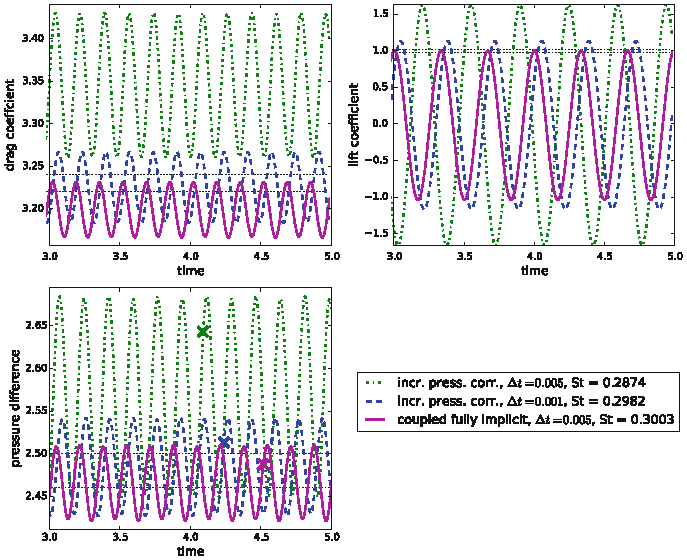
\includegraphics[width=\linewidth]{figures/Chapter_07/Fig_7_11__PDFp454__Bookp444.pdf}
\captionof{figure}{例题\hyperref[ex:incremental-pressure-correction-bdf2-cylinder]{7.101}:感兴趣量.表\hyperref[tab:appendix-d-2]{D.2}中的参考区间以点线表示;叉号标出周期的中点.Strouhal 数的参考区间为 $[0.295,0.305]$.}
\label{fig:incremental-pressure-correction-bdf2-quantities}
\end{elegantfigure}

首先,第 3 层和第 4 层网格上的结果图与图\hyperref[fig:incremental-pressure-correction-bdf2-quantities]{7.11}十分相似.因此可以看到,对全隐式方法而言,时间步长 $\Delta t=0.005$ 已足以使所有感兴趣量都落在参考区间内;而对增量压力修正格式,采用同样的时间步长会得到很不准确的结果.减小时间步长会显著提高精度;但即使取 $\Delta t=0.001$,大多数感兴趣量仍未进入各自的参考区间.总的来说,本例表明,对增量压力修正格式而言,时间离散误差占主导地位.
\end{example}
\index{压力修正格式!标准增量格式!数值结果}
